%!TEX root = ../dissertation.tex
\chapter{Boosted control region kinematic distributions}
\label{AppendixCR}

\paragraph{}
This section shows comparisons of data with the prediction of QCD multi-jets and \ttbar~ backgrounds in the control region. 
The definition of the control region is discussed in Section~\ref{sec:boosted-SBCR}.
The agreement between data and background prediction is generally good, without any systematic biases observed.

\paragraph{}
Figures~\ref{fig:boosted-4b-control-ak10-lead}, \ref{fig:boosted-4b-control-ak10-subl}, \ref{fig:boosted-4b-control-ak2}, and \ref{fig:boosted-4b-control-ak10-system} show predictions of various kinematics of the large-\R jets and their associated track jets in the $4b$ selection. 
Figures~\ref{fig:boosted-3b-control-ak10-lead}, \ref{fig:boosted-3b-control-ak10-subl}, \ref{fig:boosted-3b-control-ak2},  and \ref{fig:boosted-3b-control-ak10-system} show predictions of various kinematics of the large-\R jets and their associated track jets in the $3b$ selection. 
Figures~\ref{fig:boosted-2bs-control-ak10-lead}, \ref{fig:boosted-2bs-control-ak10-subl}, \ref{fig:boosted-2bs-control-ak2},  and \ref{fig:boosted-2bs-control-ak10-system} show predictions of various kinematics of the large-\R jets and their associated track jets in the $2bs$ selection.

\begin{figure*}[htbp!]
\begin{center}
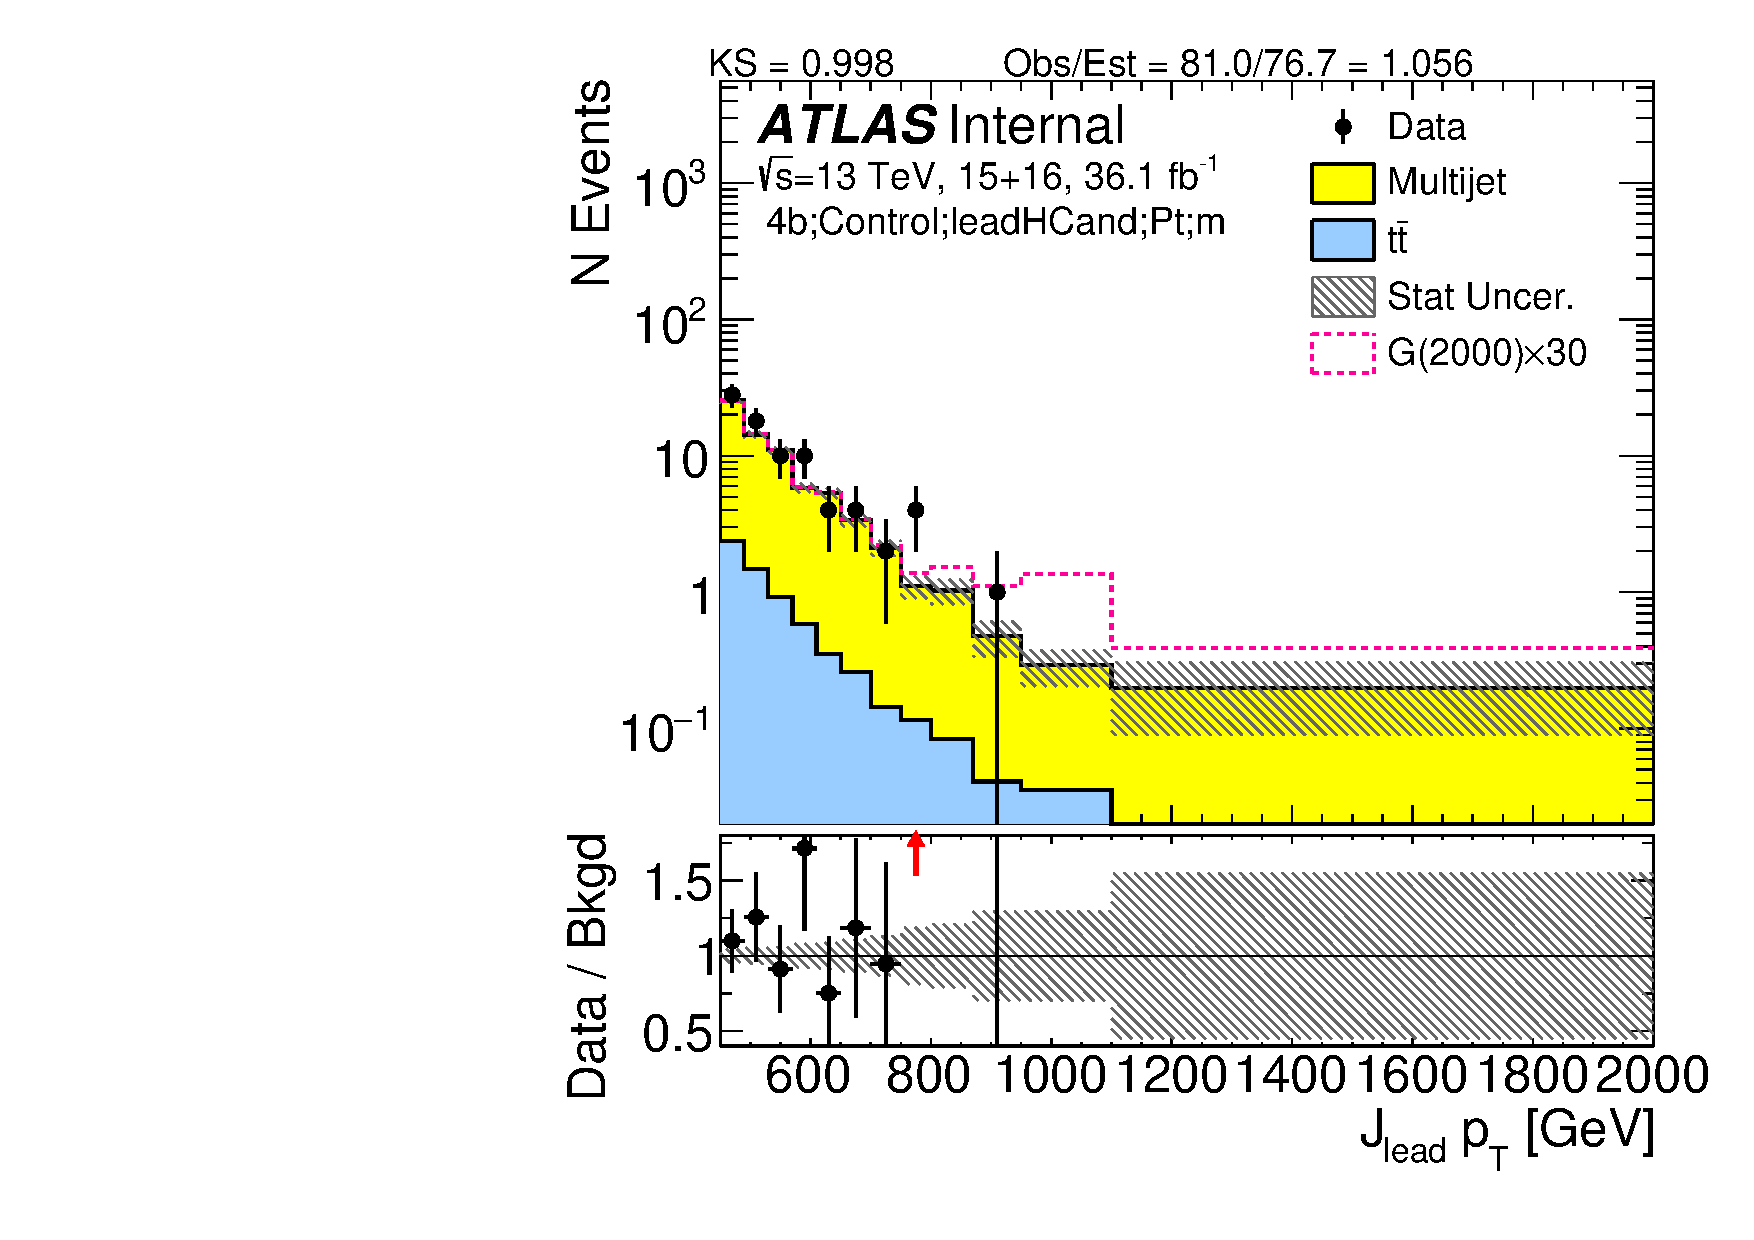
\includegraphics[width=0.32\textwidth,angle=-90]{figures/boosted/Control/b77_FourTag_Control_leadHCand_Pt_m_1.pdf}
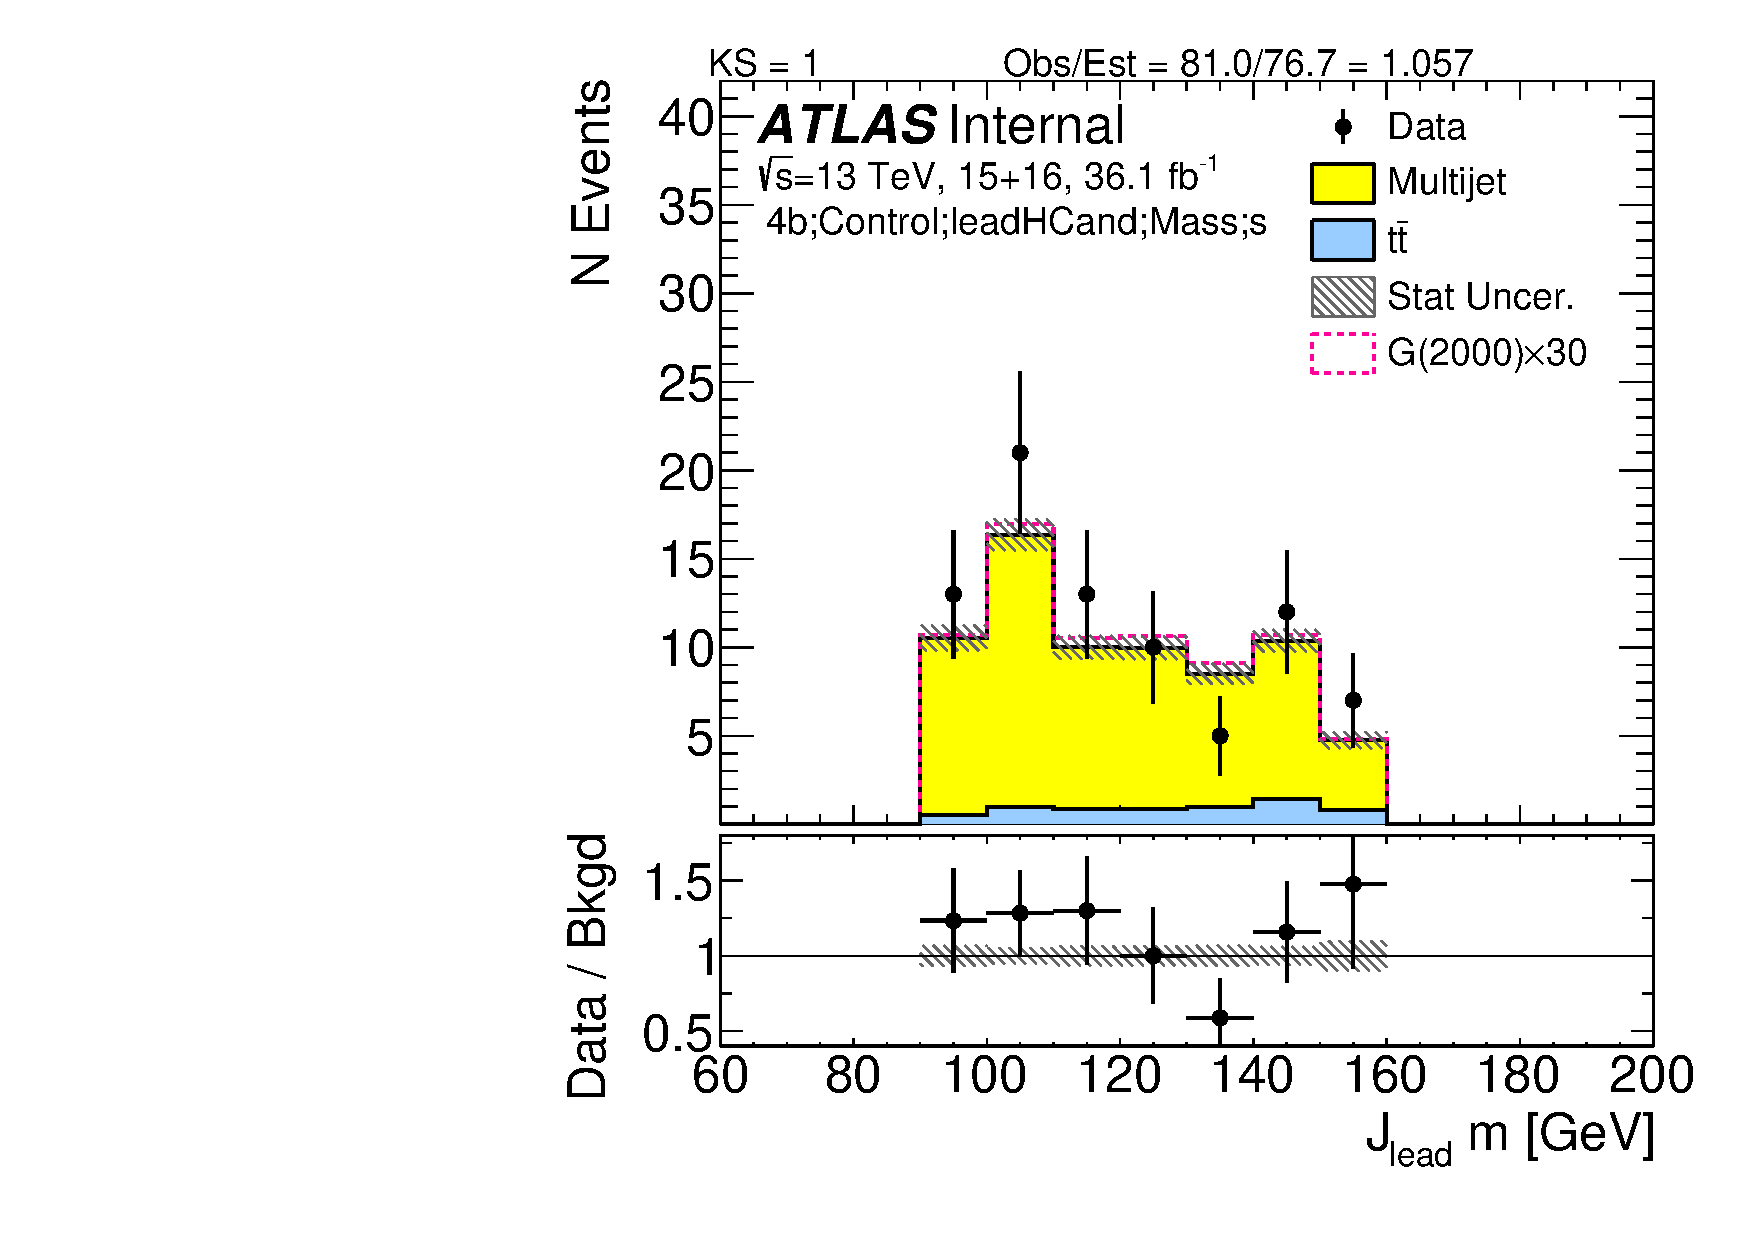
\includegraphics[width=0.32\textwidth,angle=-90]{figures/boosted/Control/b77_FourTag_Control_leadHCand_Mass_s.pdf}\\
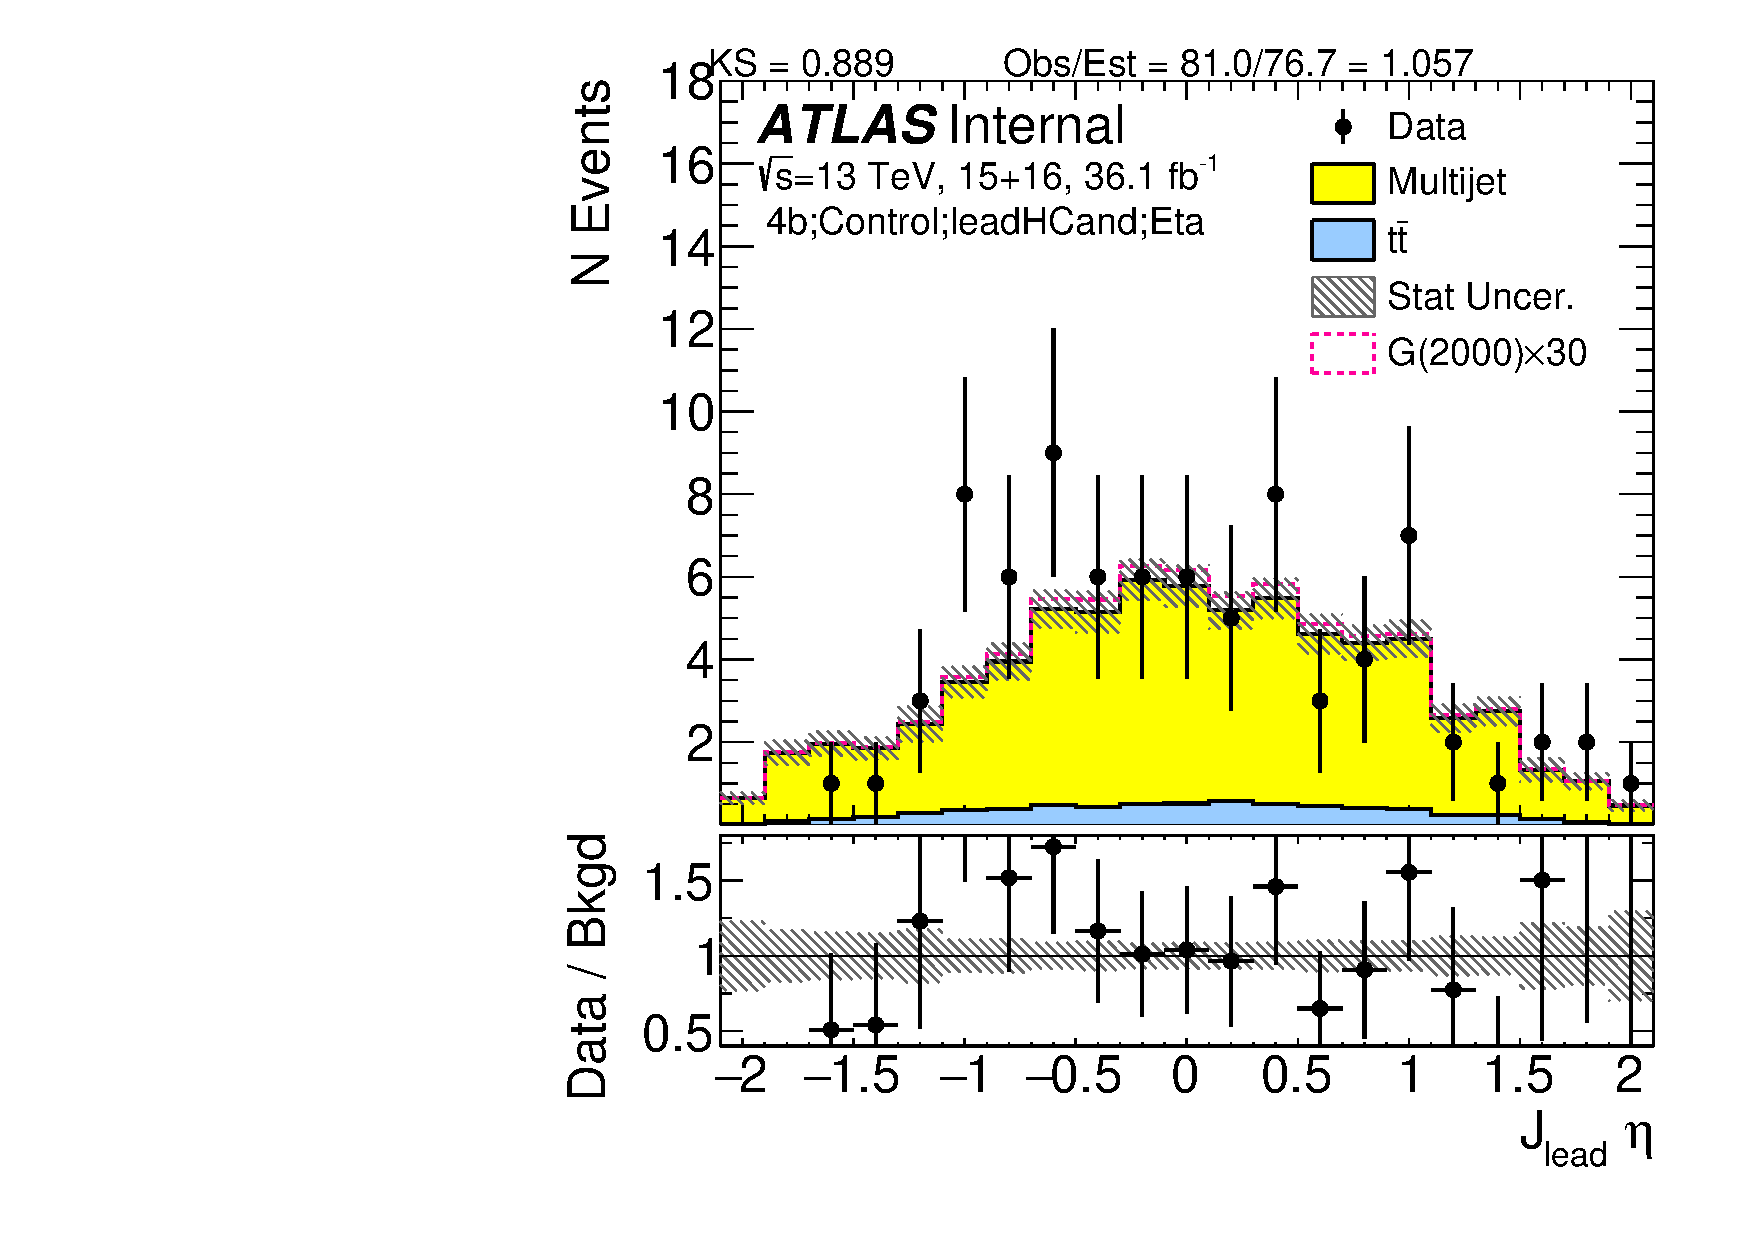
\includegraphics[width=0.32\textwidth,angle=-90]{figures/boosted/Control/b77_FourTag_Control_leadHCand_Eta.pdf}
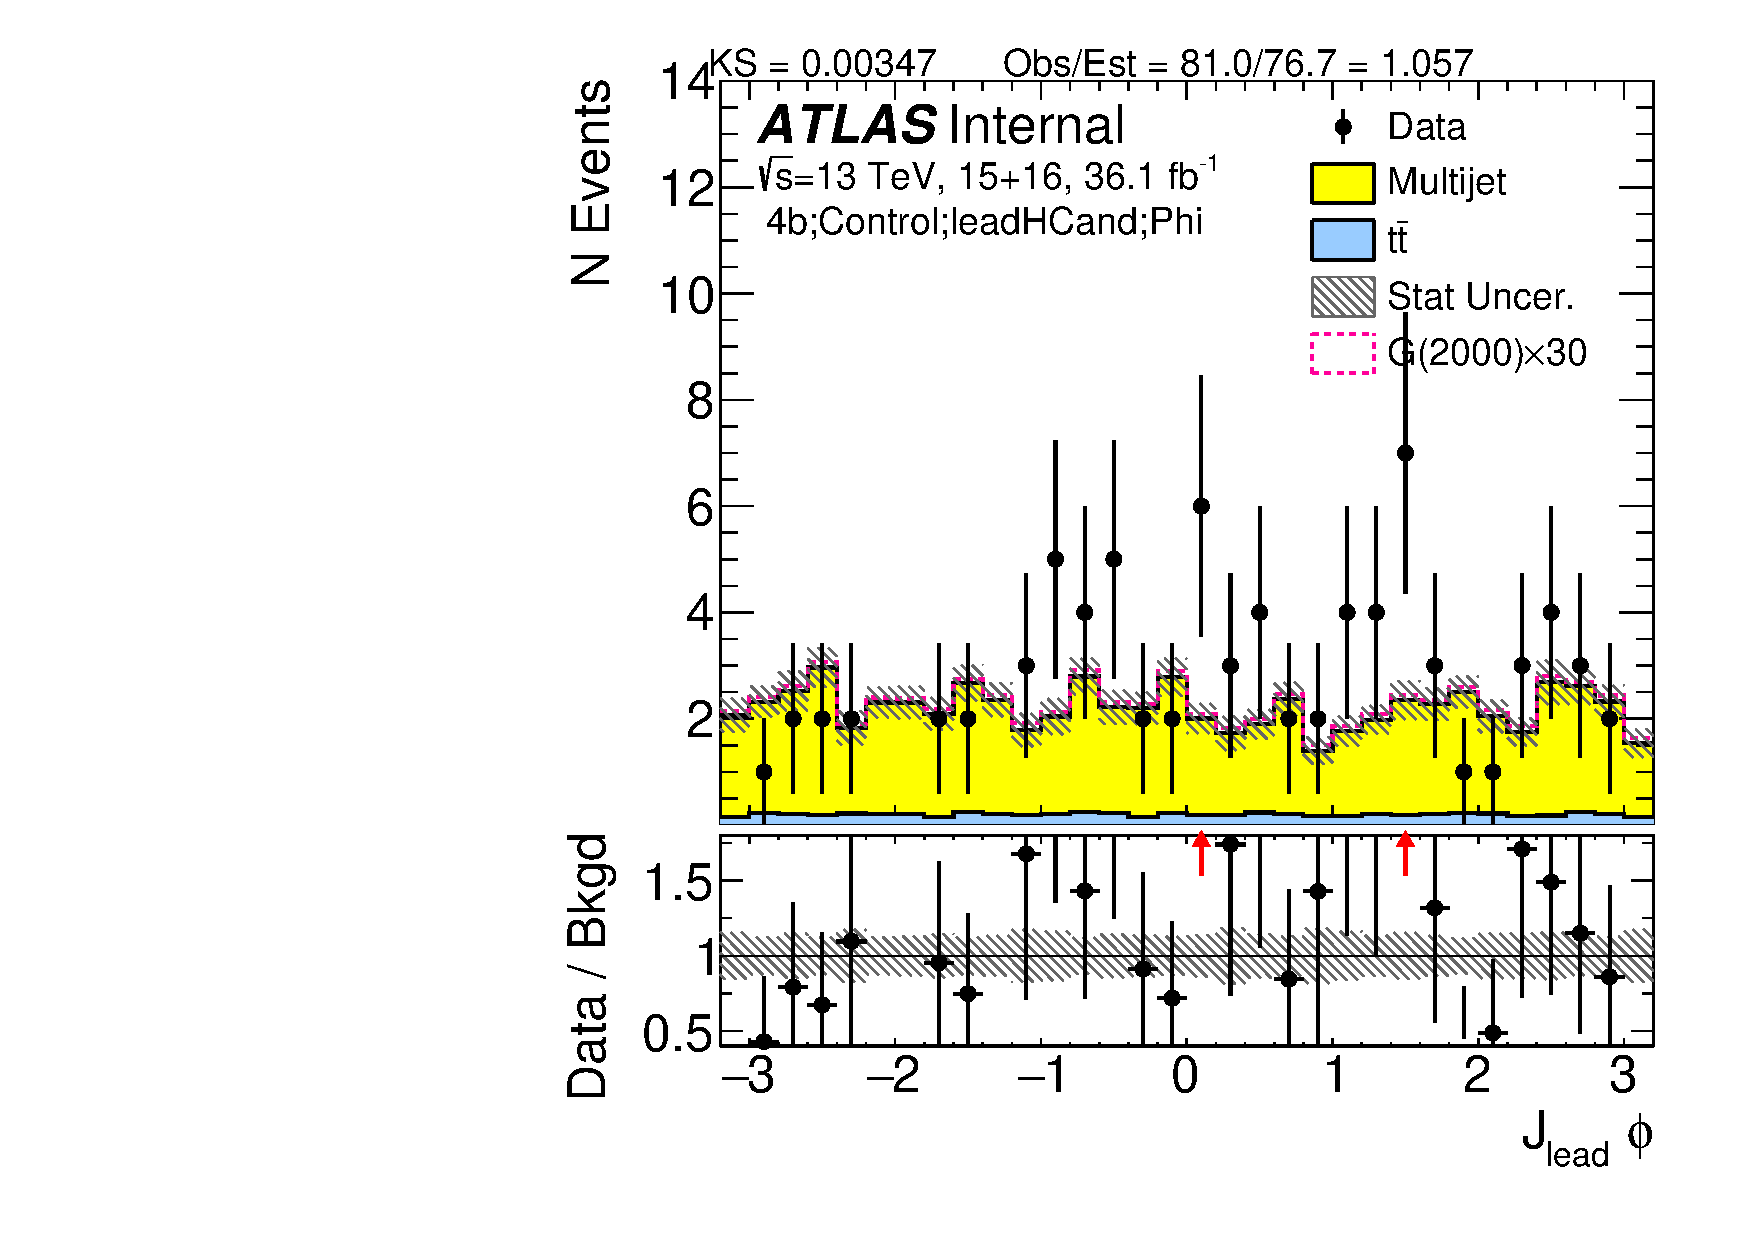
\includegraphics[width=0.32\textwidth,angle=-90]{figures/boosted/Control/b77_FourTag_Control_leadHCand_Phi.pdf}
  \caption{Kinematics of the lead large-\R jet in data and prediction in the control region after requiring 4 $b$-tags. }
  \label{fig:boosted-4b-control-ak10-lead}
\end{center}
\end{figure*}

\begin{figure*}[htbp!]
\begin{center}
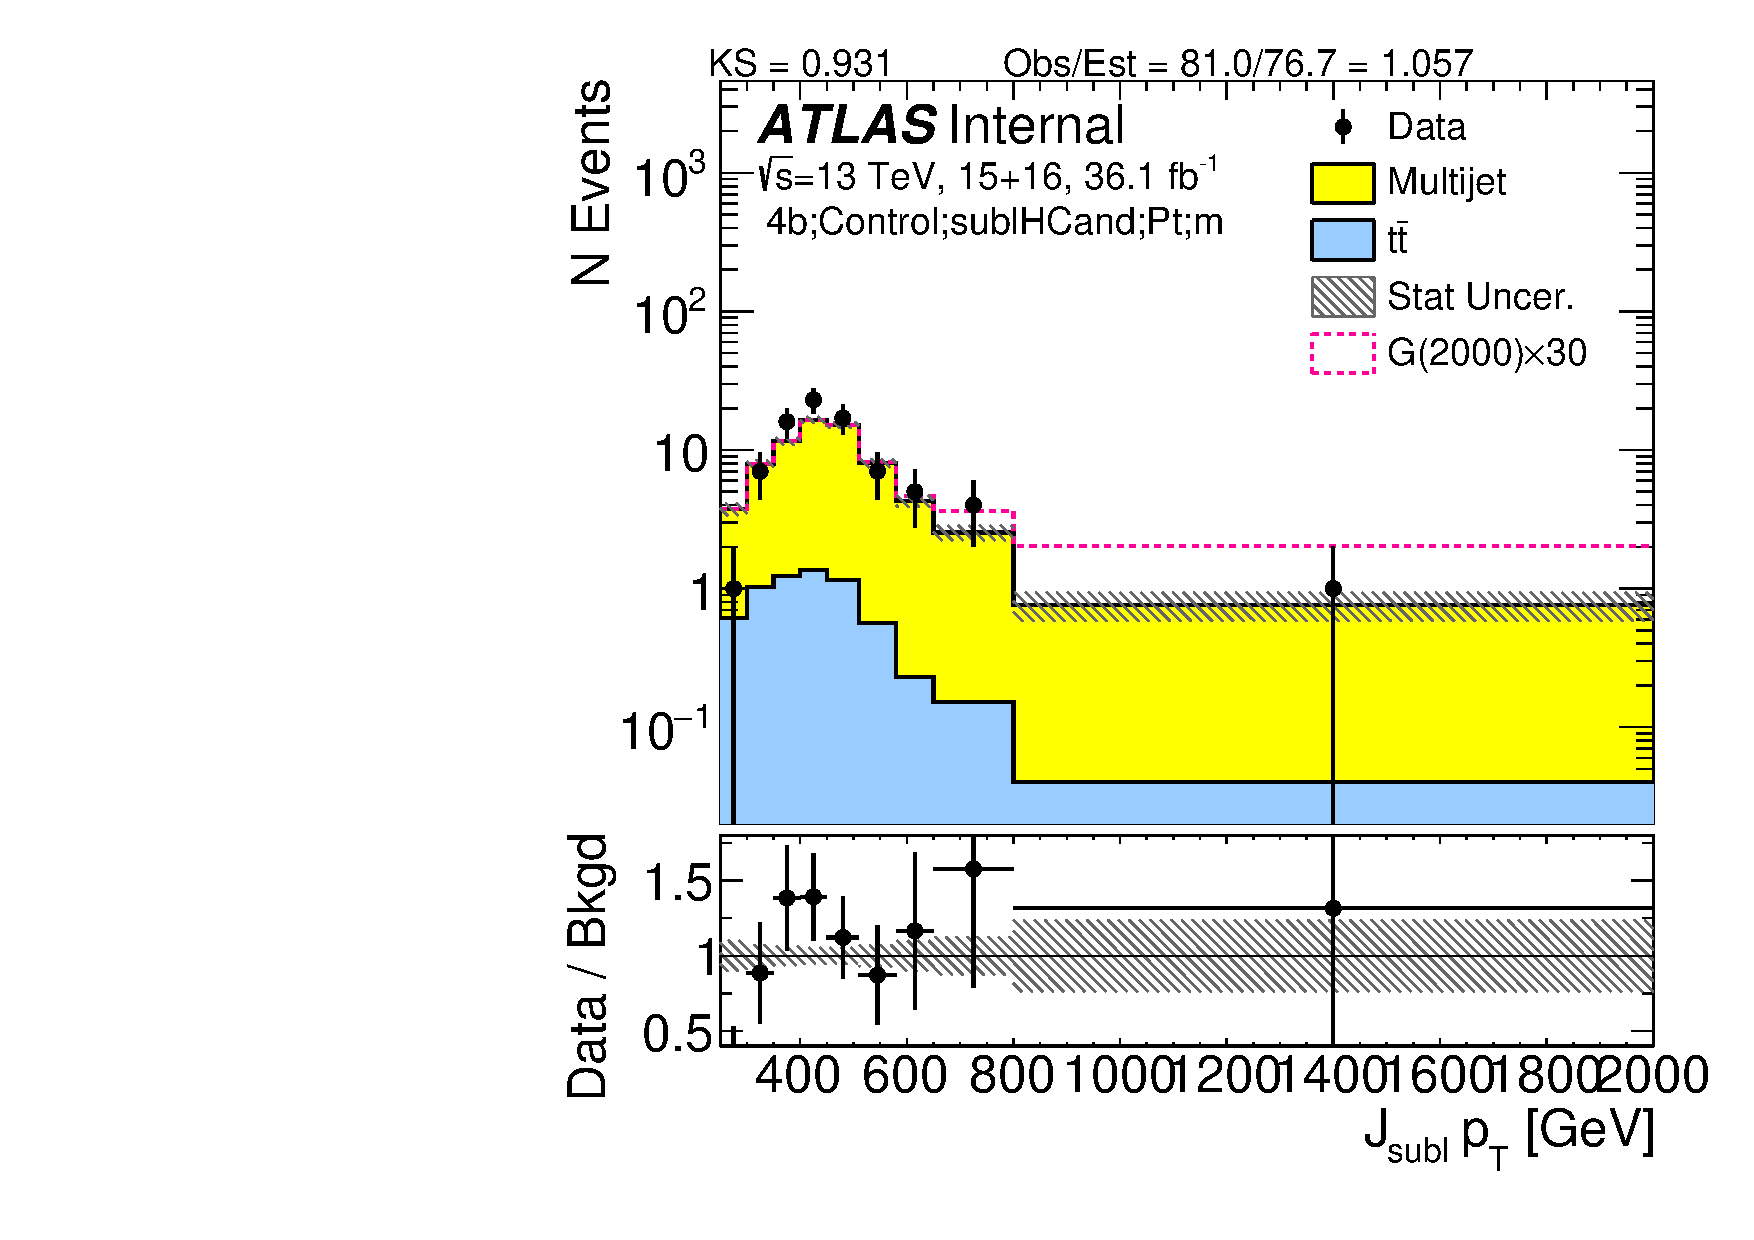
\includegraphics[width=0.32\textwidth,angle=-90]{figures/boosted/Control/b77_FourTag_Control_sublHCand_Pt_m_1.pdf}
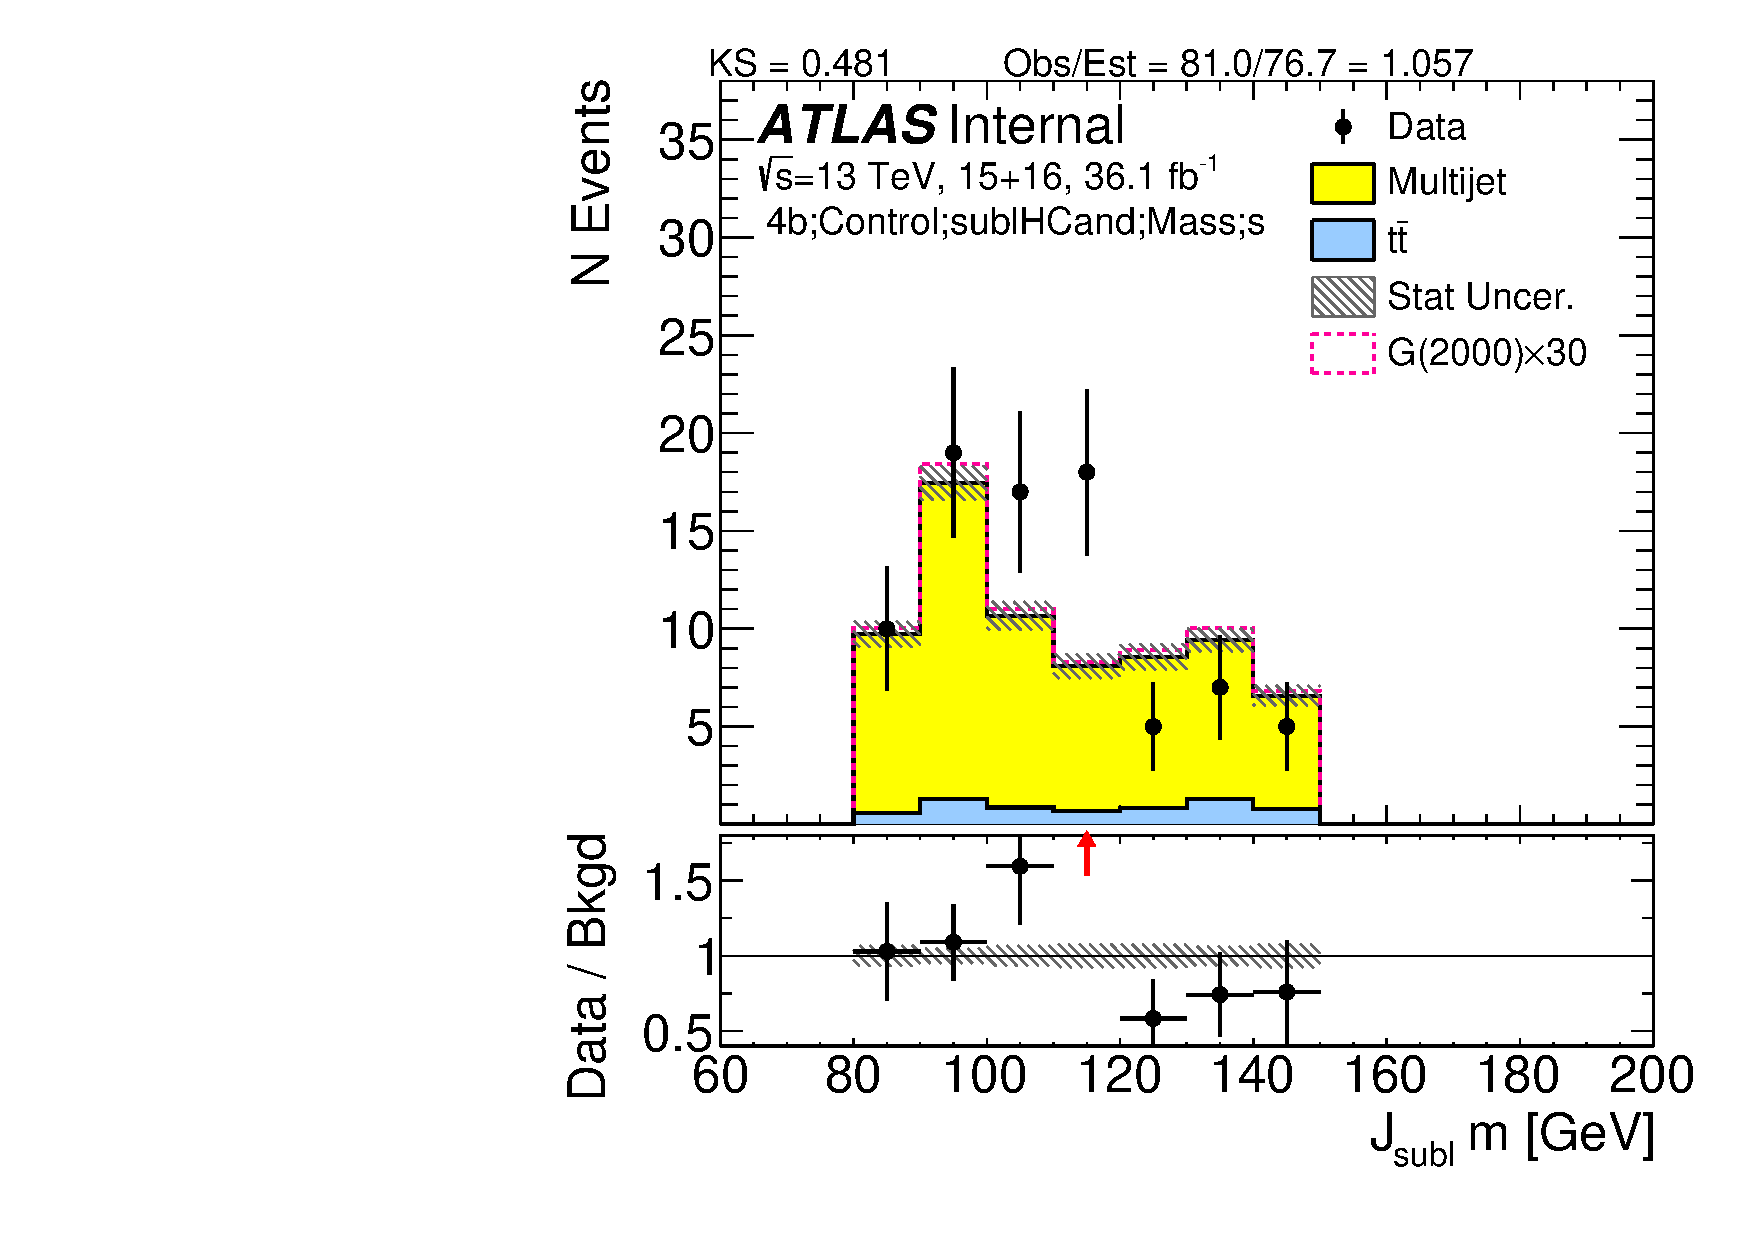
\includegraphics[width=0.32\textwidth,angle=-90]{figures/boosted/Control/b77_FourTag_Control_sublHCand_Mass_s.pdf}\\
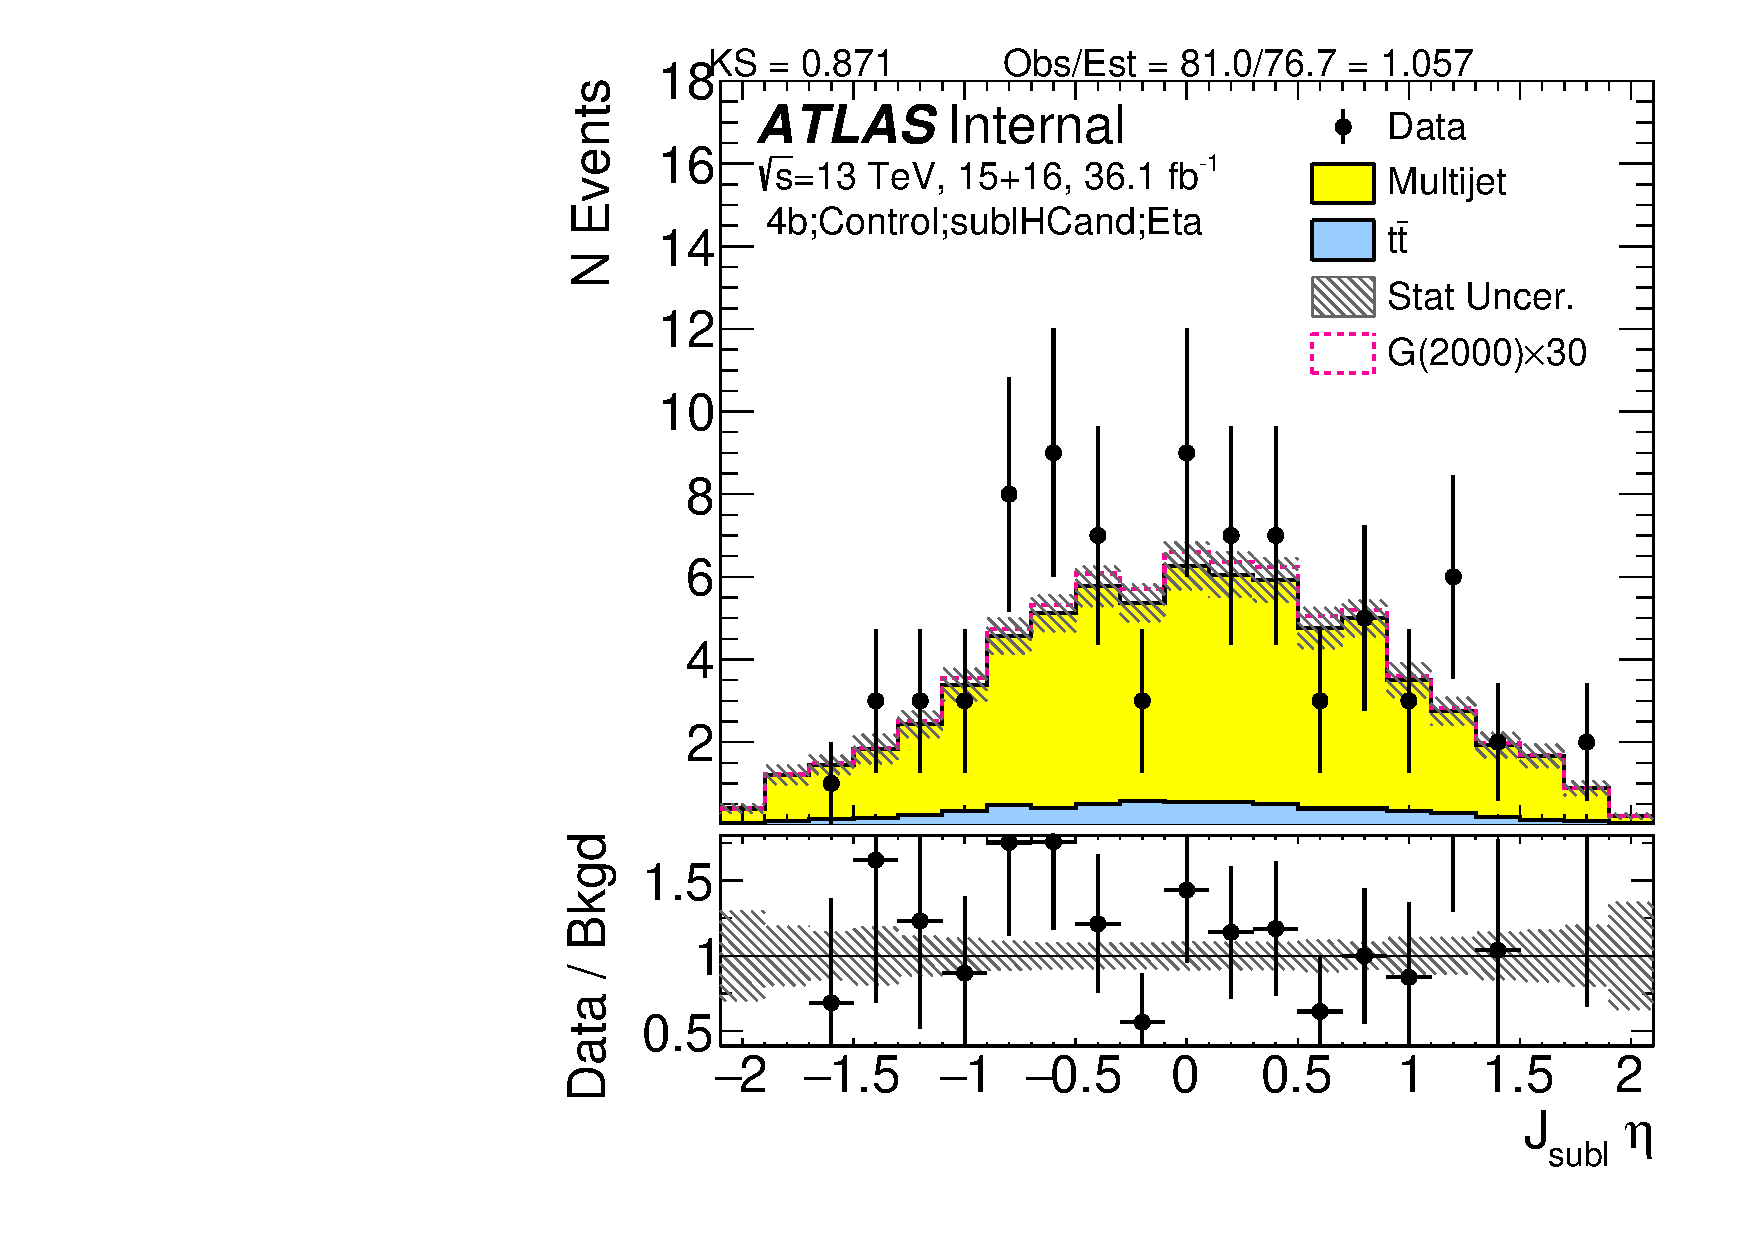
\includegraphics[width=0.32\textwidth,angle=-90]{figures/boosted/Control/b77_FourTag_Control_sublHCand_Eta.pdf}
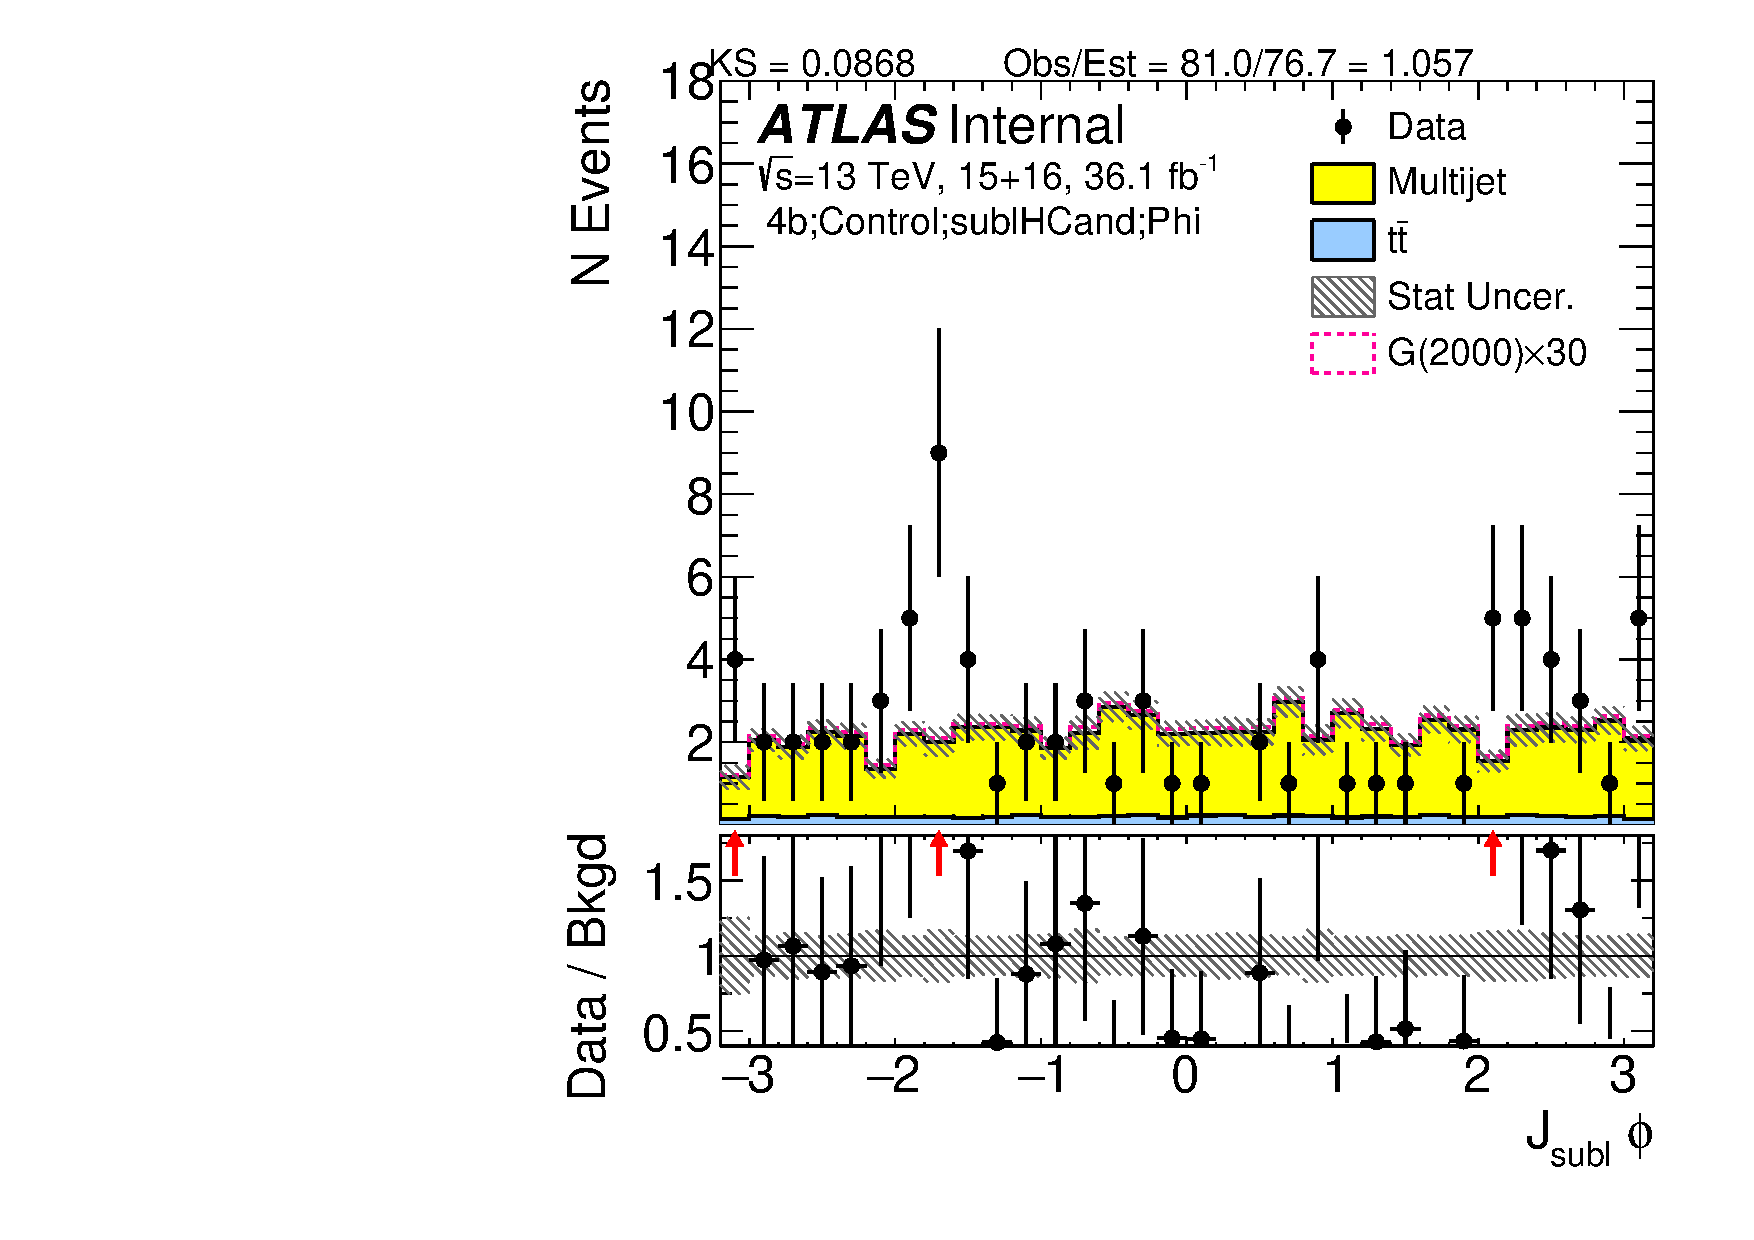
\includegraphics[width=0.32\textwidth,angle=-90]{figures/boosted/Control/b77_FourTag_Control_sublHCand_Phi.pdf}
  \caption{Kinematics of the sub-lead large-\R jet in data and prediction in the control region after requiring 4 $b$-tags. }
  \label{fig:boosted-4b-control-ak10-subl}
\end{center}
\end{figure*}

\begin{figure*}[htbp!]
\begin{center}
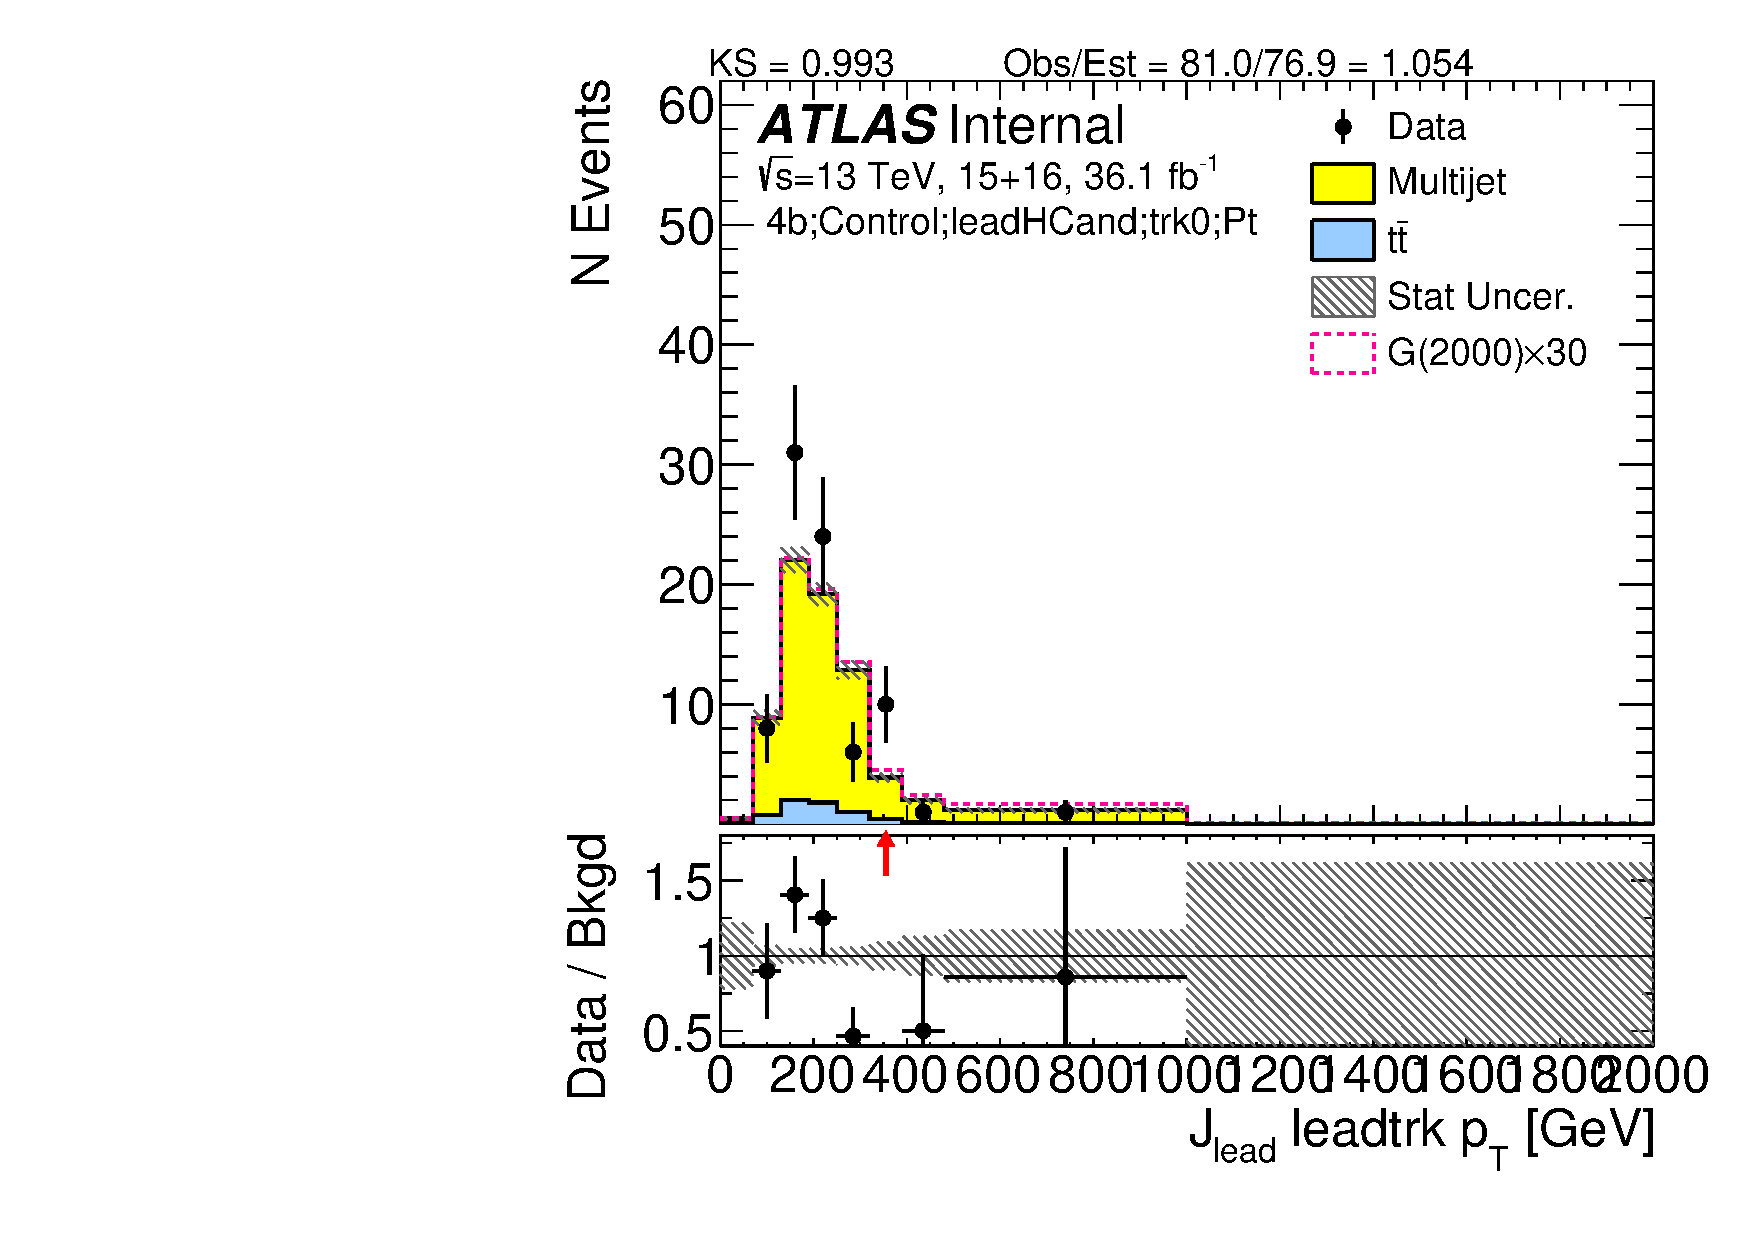
\includegraphics[width=0.32\textwidth,angle=-90]{figures/boosted/Control/b77_FourTag_Control_leadHCand_trk0_Pt.pdf}
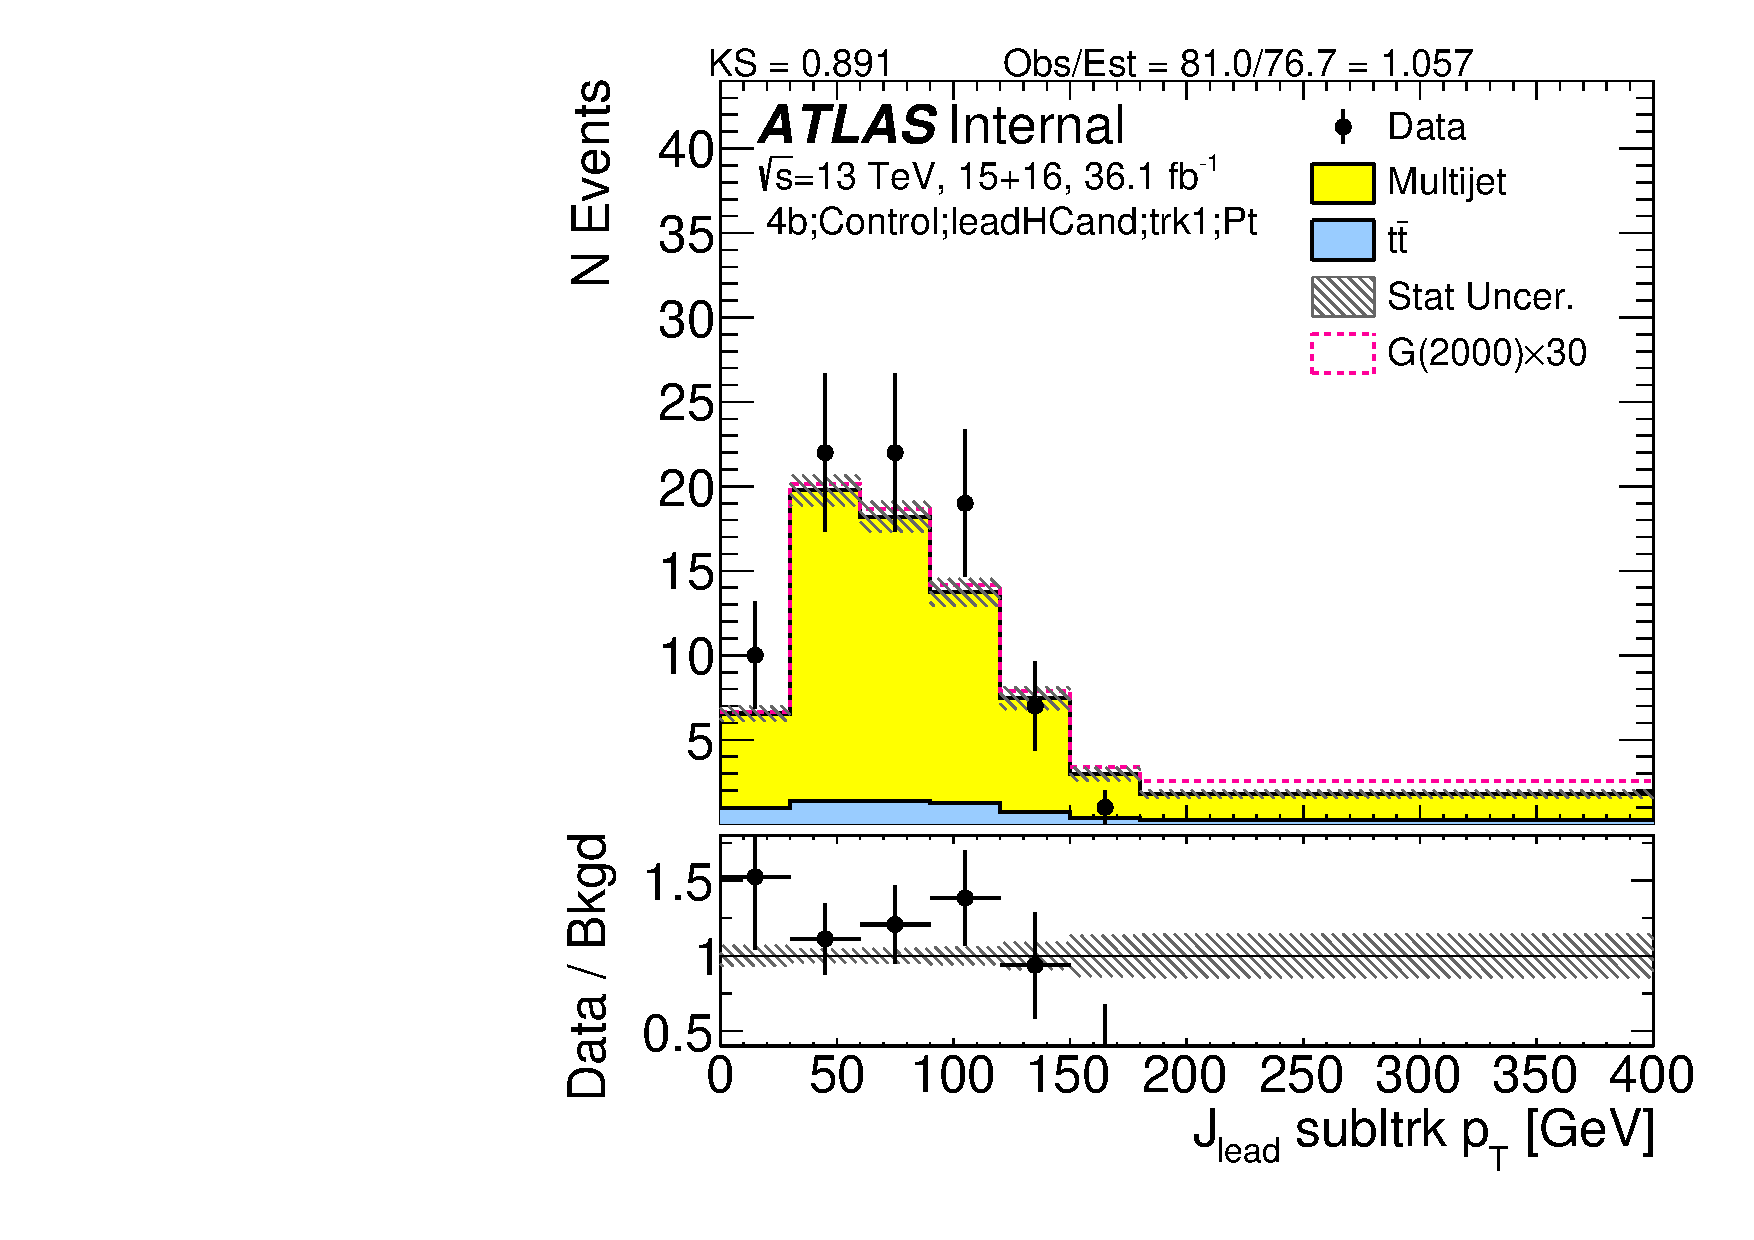
\includegraphics[width=0.32\textwidth,angle=-90]{figures/boosted/Control/b77_FourTag_Control_leadHCand_trk1_Pt.pdf}\\
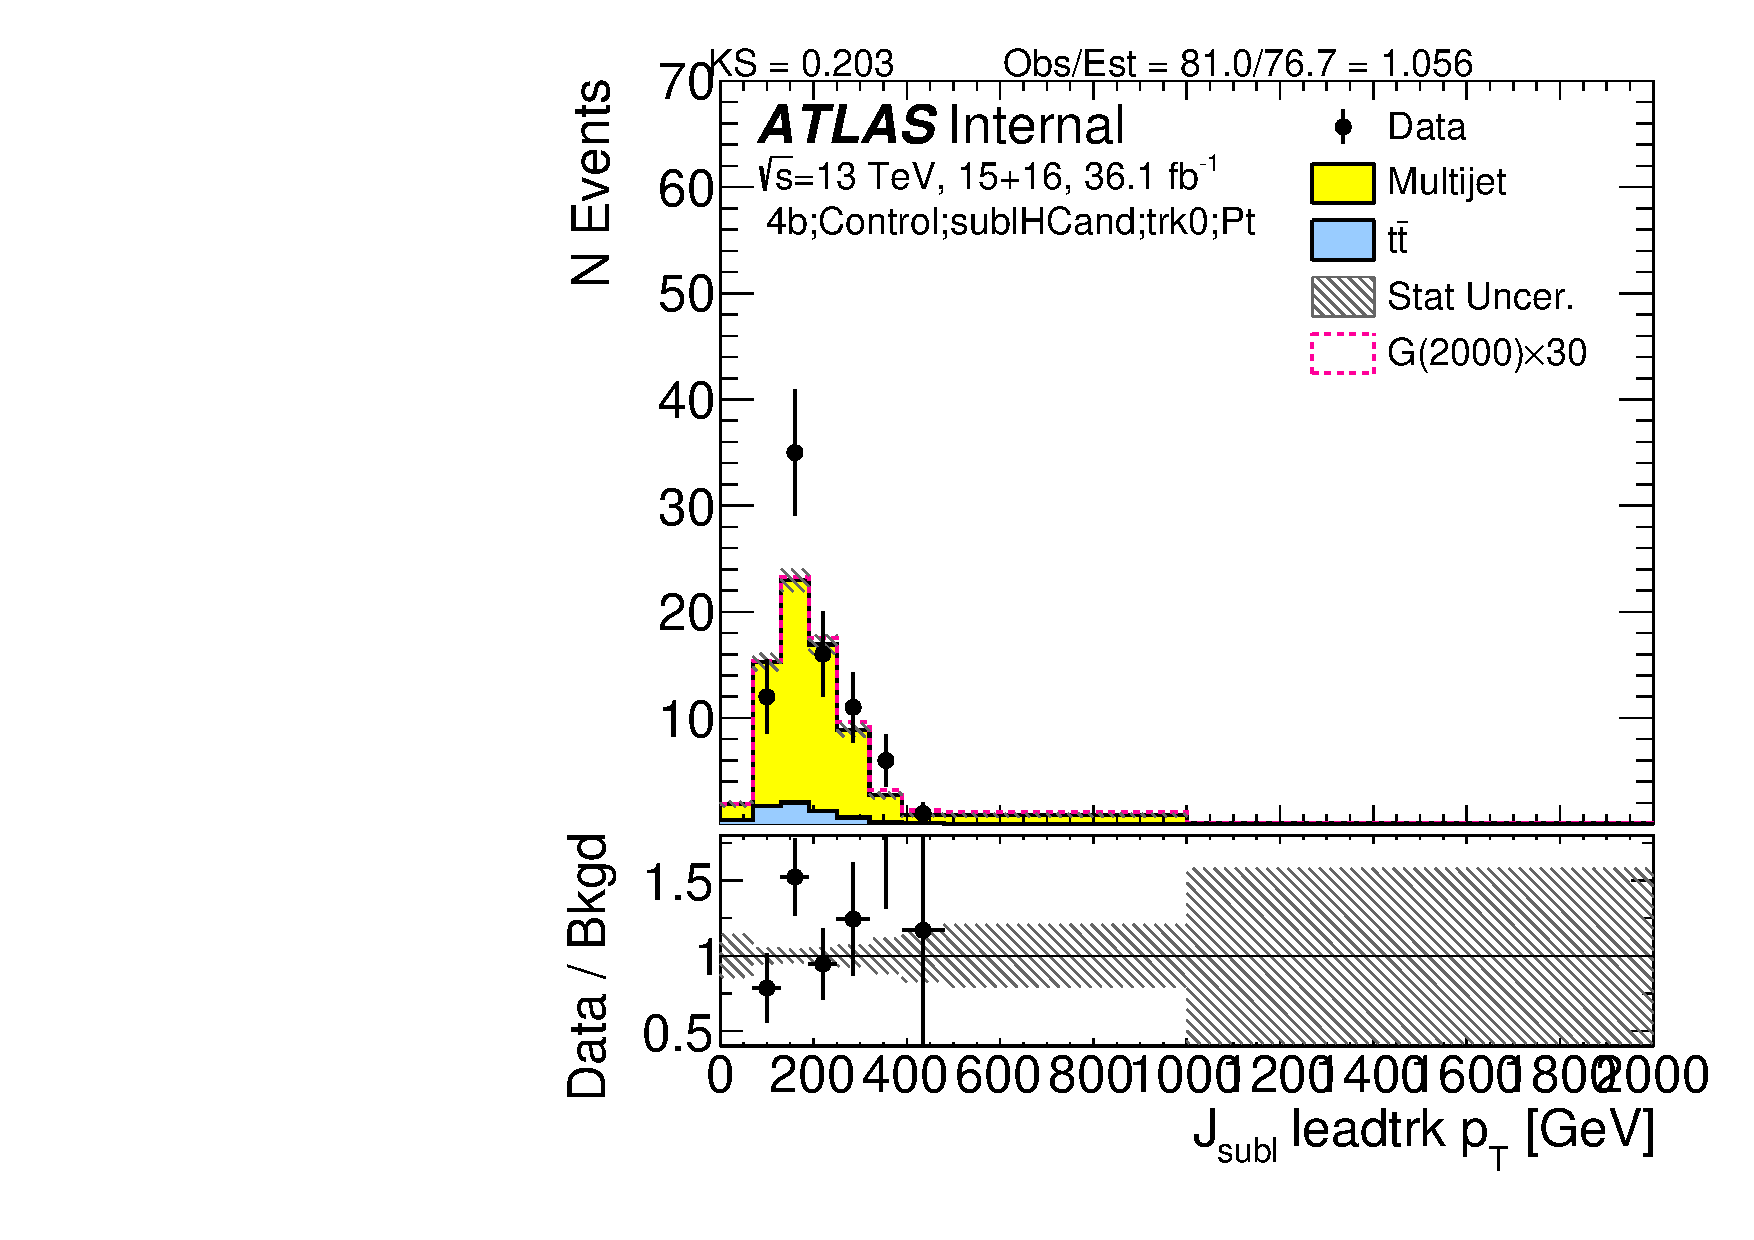
\includegraphics[width=0.32\textwidth,angle=-90]{figures/boosted/Control/b77_FourTag_Control_sublHCand_trk0_Pt.pdf}
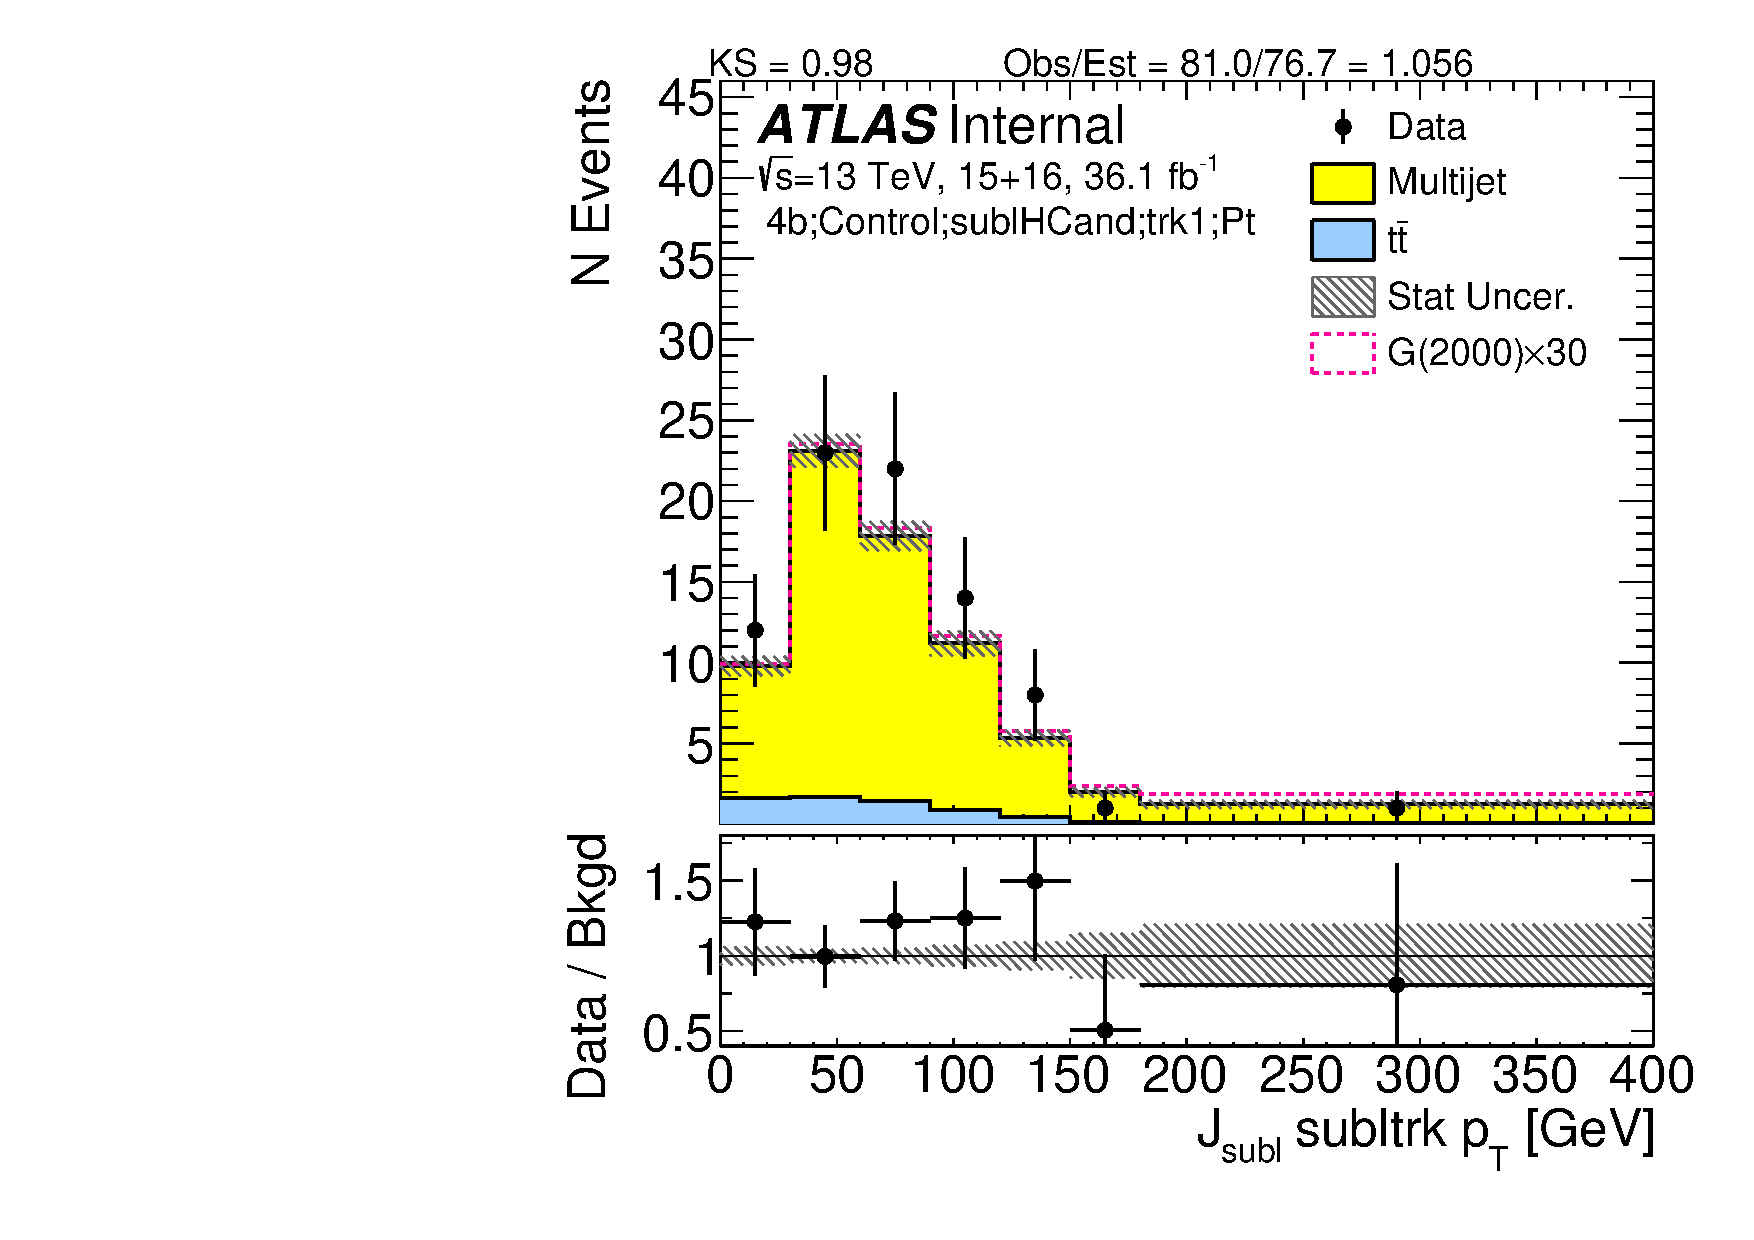
\includegraphics[width=0.32\textwidth,angle=-90]{figures/boosted/Control/b77_FourTag_Control_sublHCand_trk1_Pt.pdf}\\
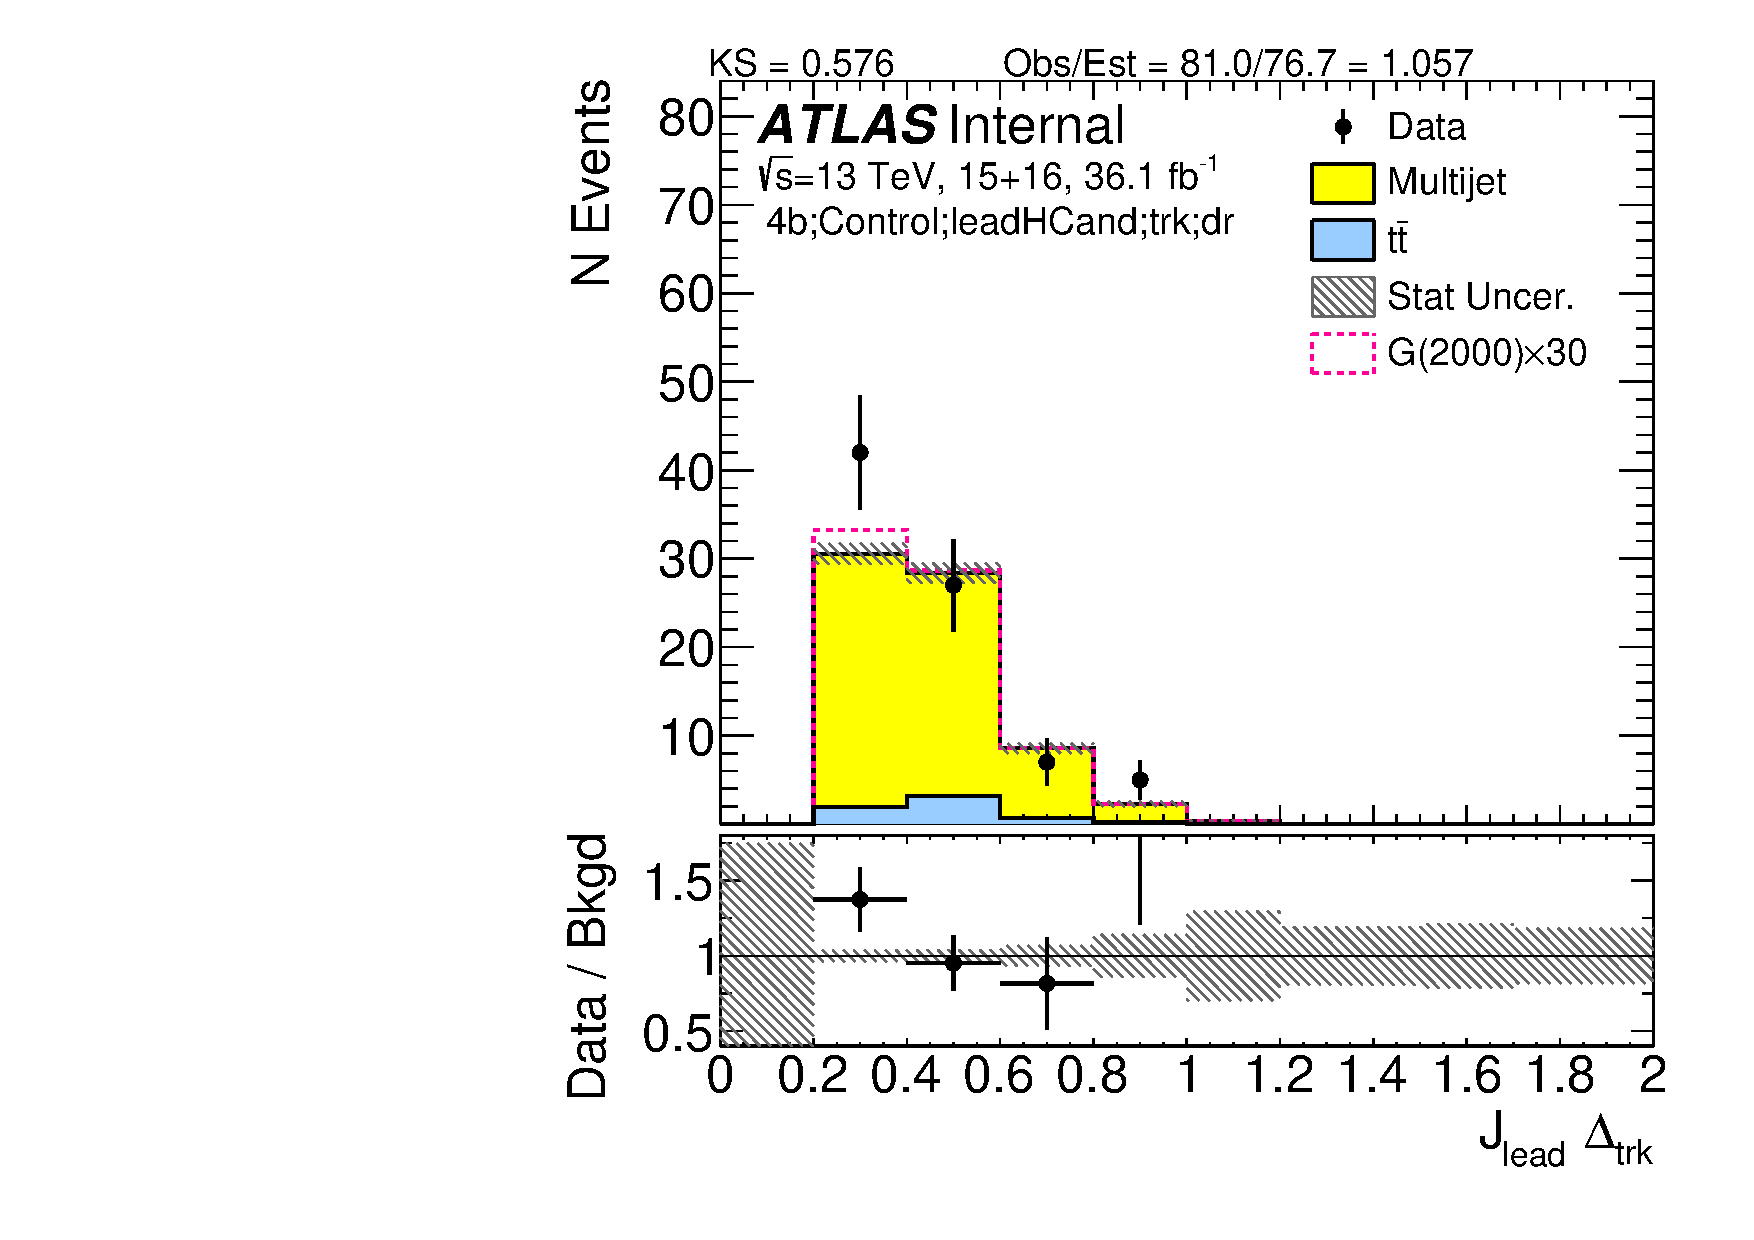
\includegraphics[width=0.32\textwidth,angle=-90]{figures/boosted/Control/b77_FourTag_Control_leadHCand_trk_dr.pdf}
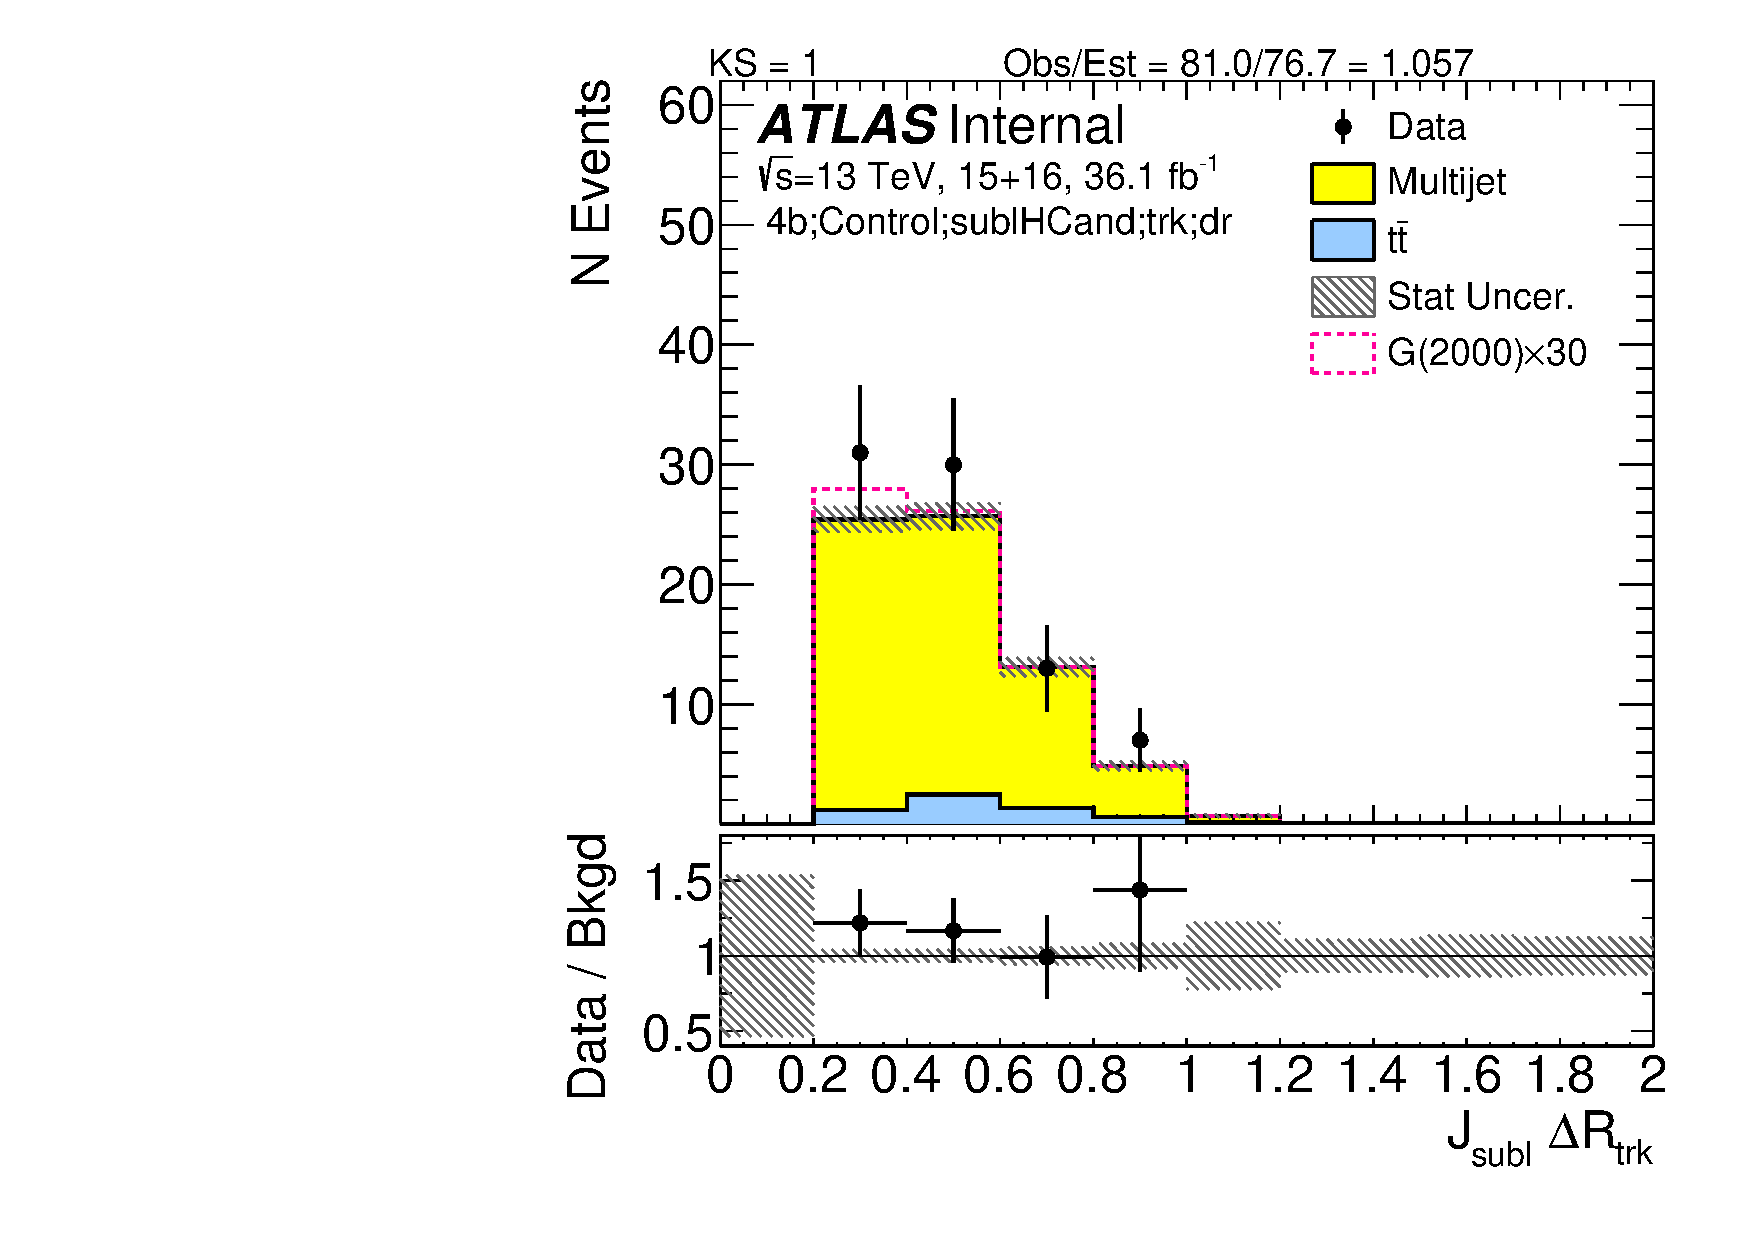
\includegraphics[width=0.32\textwidth,angle=-90]{figures/boosted/Control/b77_FourTag_Control_sublHCand_trk_dr.pdf}
  \caption{First two rows show the kinematics of the lead (left) and sub-lead (right) small-$R$ track jets associated to the lead (first-row) and sub-lead (second-row) large-\R jet in data and prediction in the control region after requiring 4 $b$-tags. Third row shows the $\Delta R$ between two leading small-$R$ track-jets associated to the leading (left) and sub-leading (right) large-\R jet.  }
  \label{fig:boosted-4b-control-ak2}
\end{center}
\end{figure*}


\begin{figure*}[htbp!]
\begin{center}
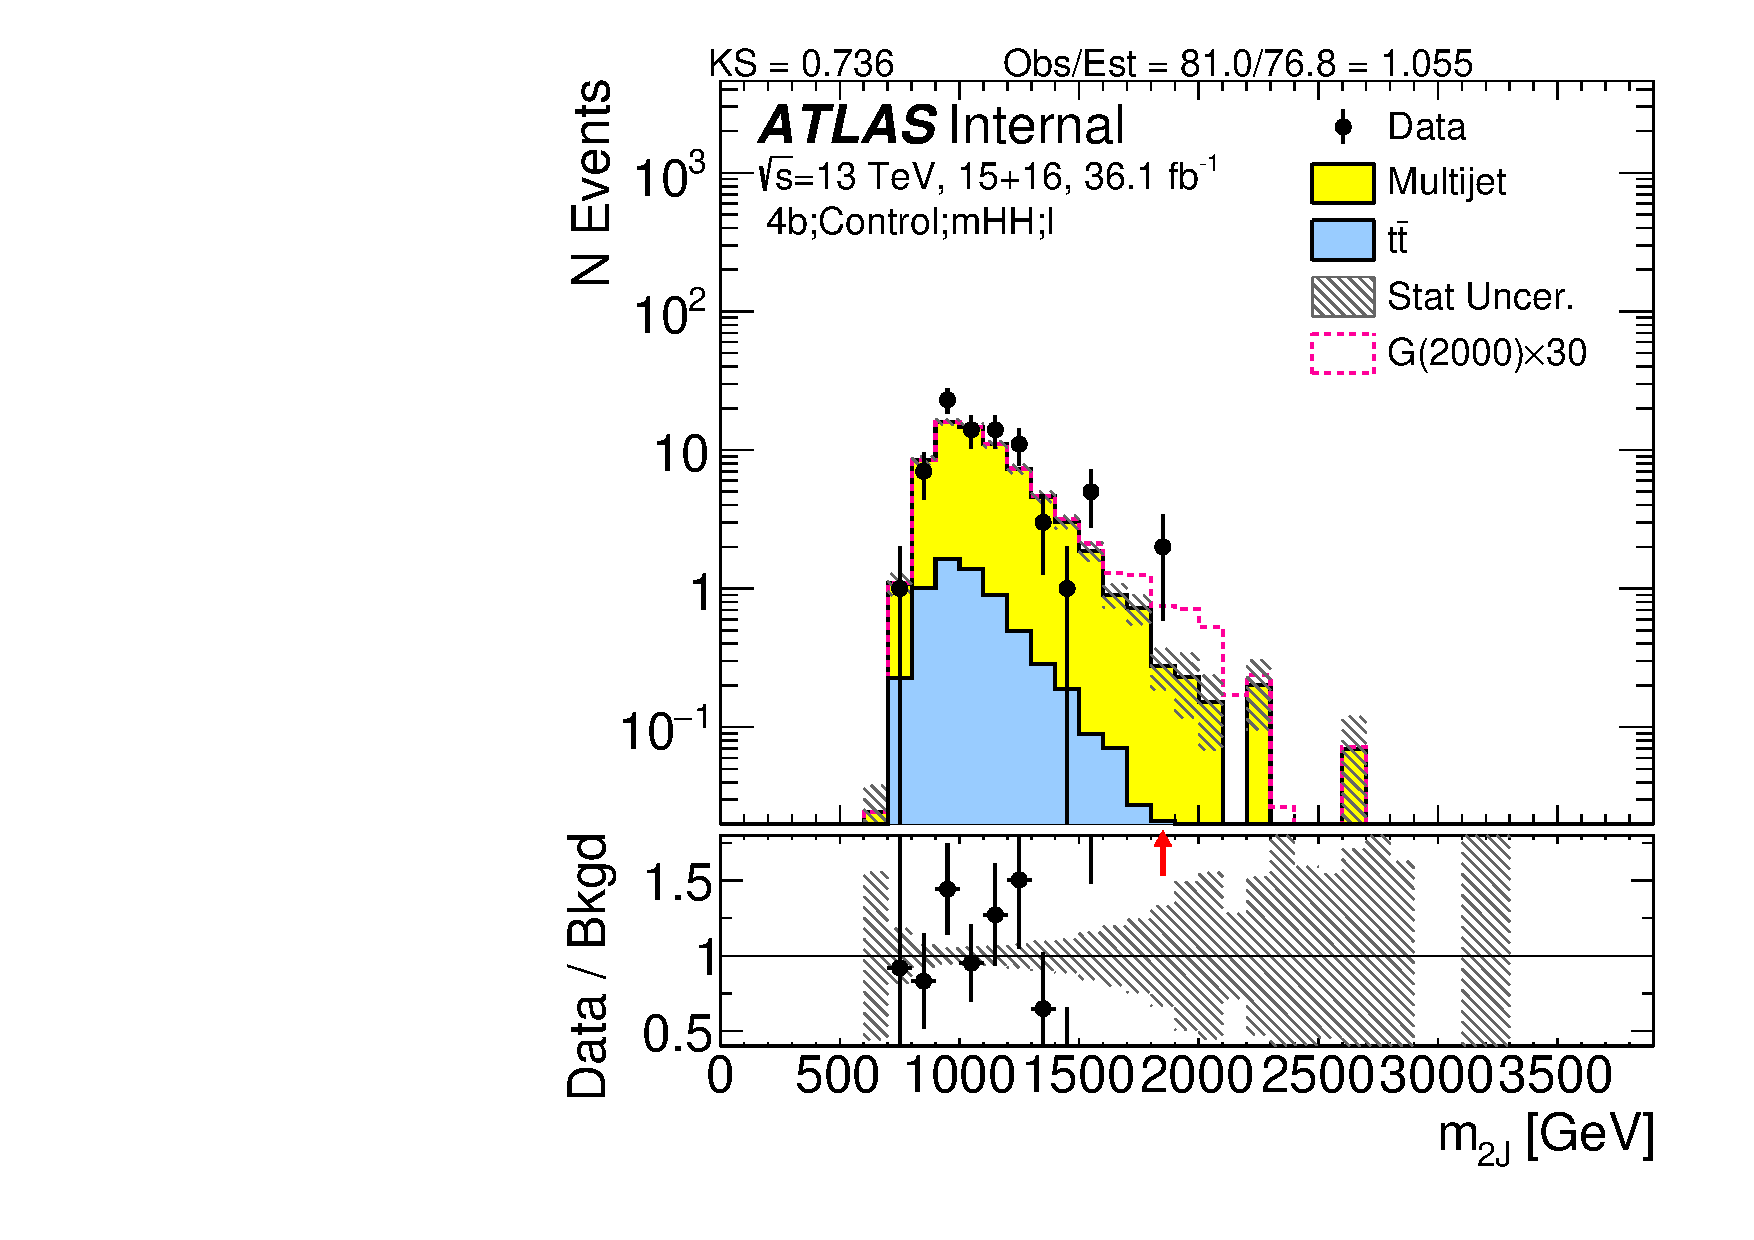
\includegraphics[width=0.32\textwidth,angle=-90]{figures/boosted/Control/b77_FourTag_Control_mHH_l_1.pdf}
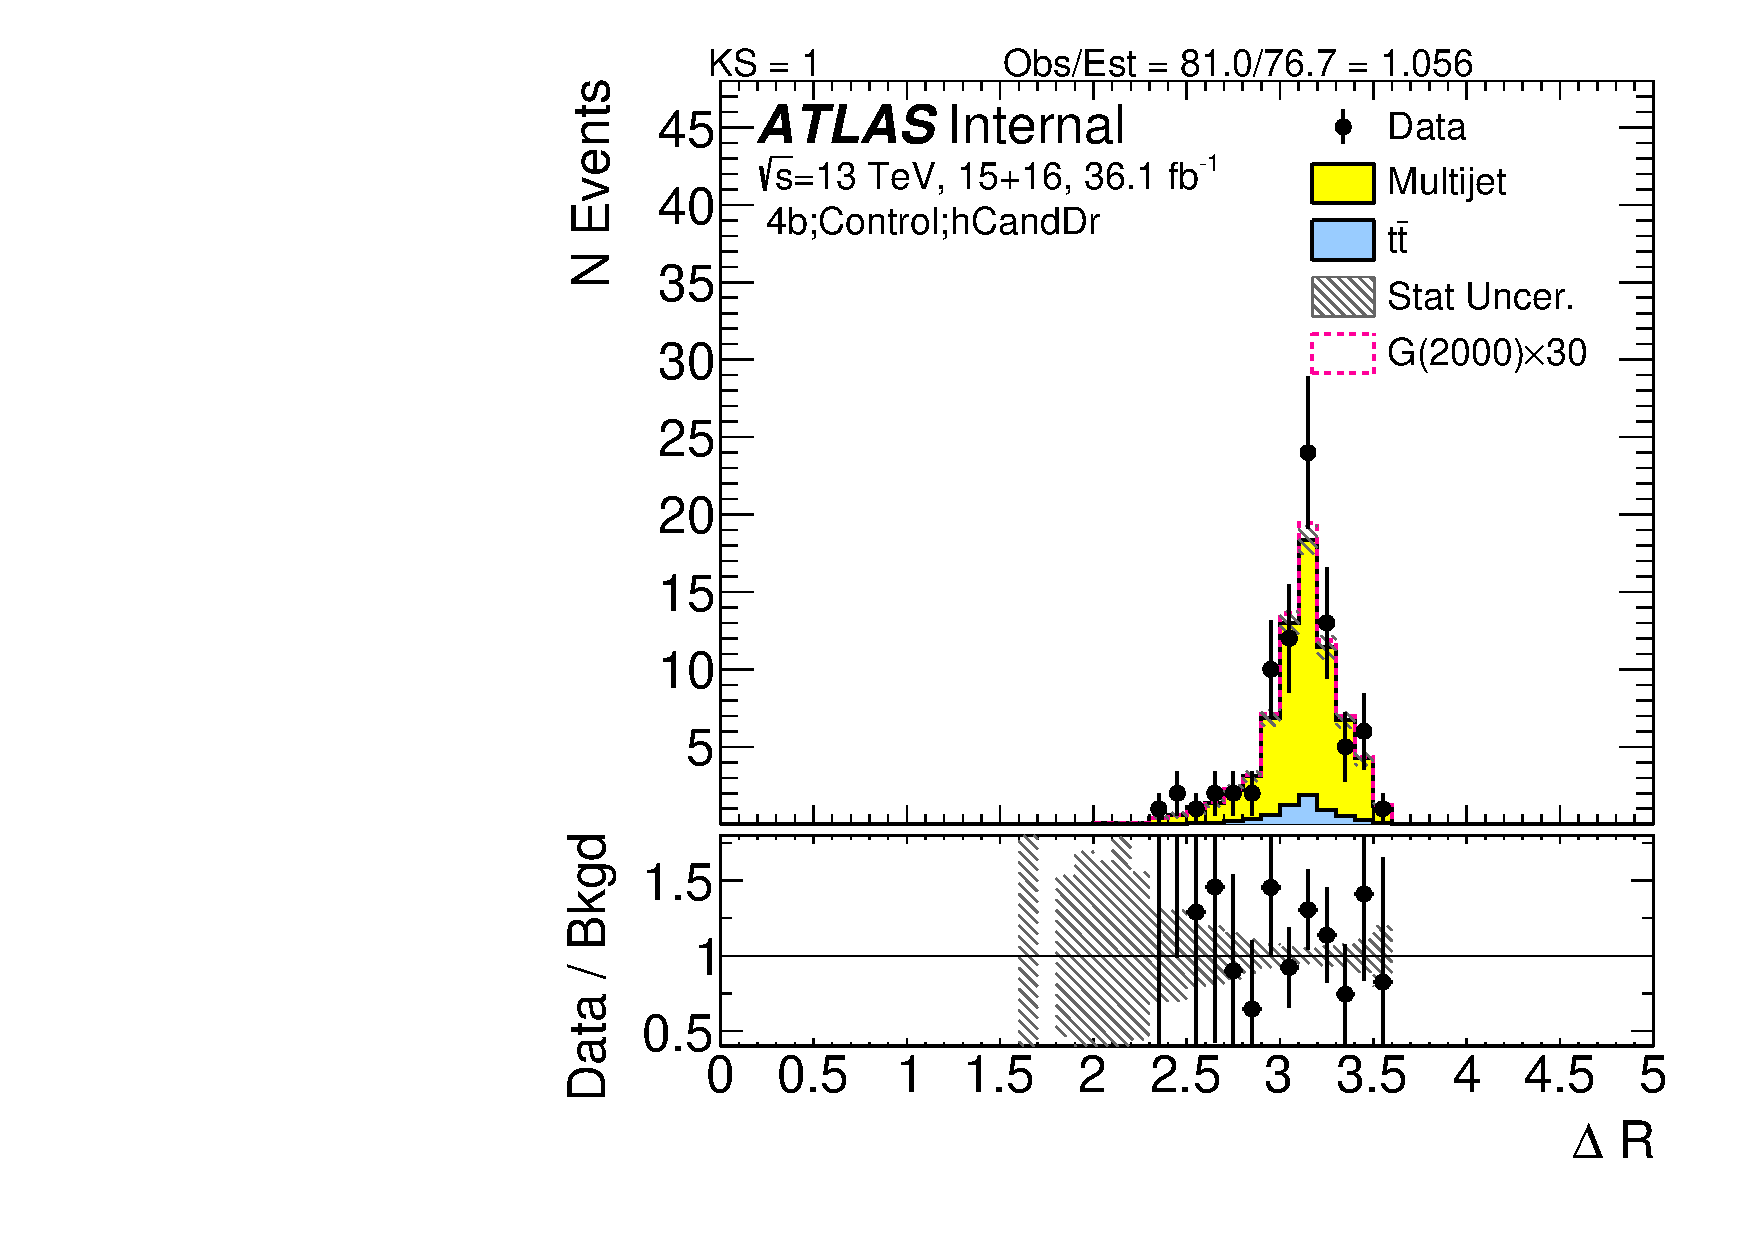
\includegraphics[width=0.32\textwidth,angle=-90]{figures/boosted/Control/b77_FourTag_Control_hCandDr.pdf}\\
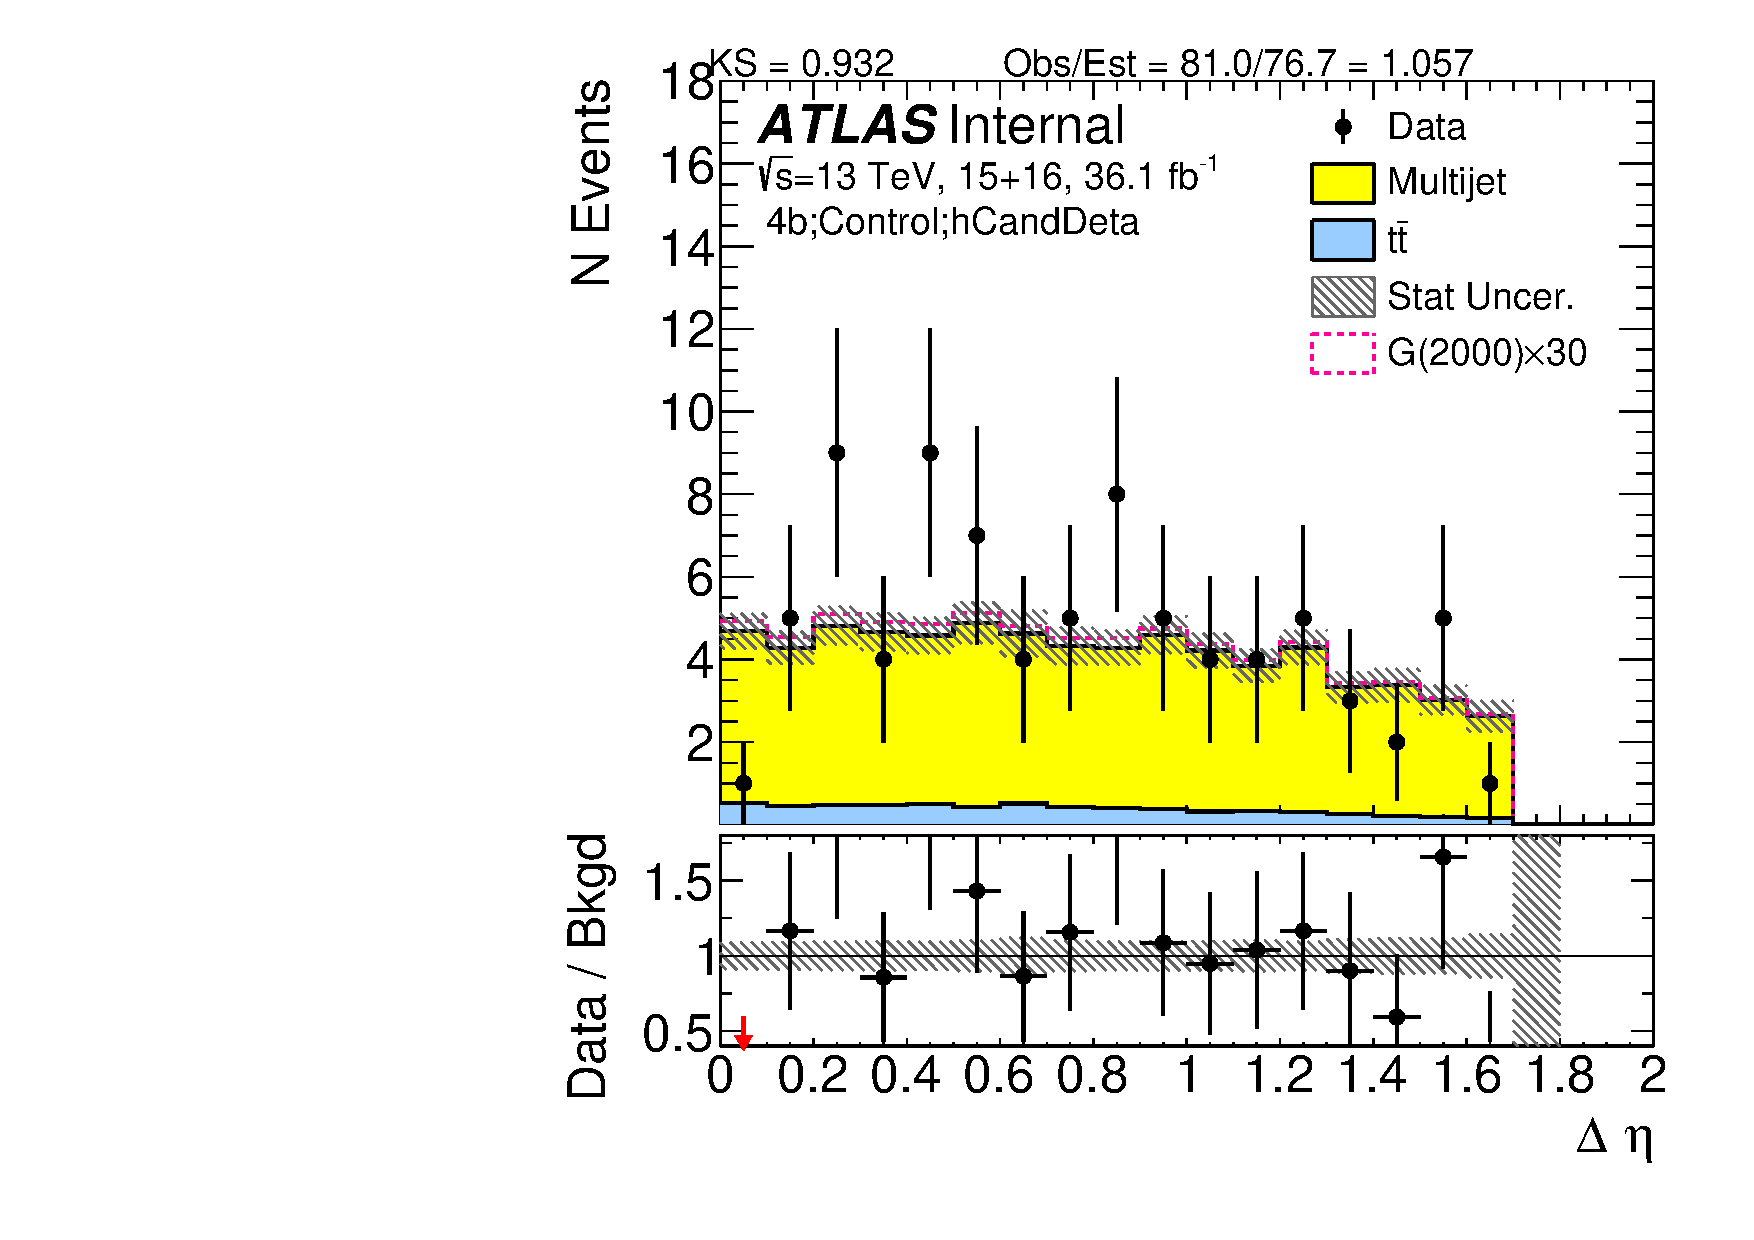
\includegraphics[width=0.32\textwidth,angle=-90]{figures/boosted/Control/b77_FourTag_Control_hCandDeta.pdf}
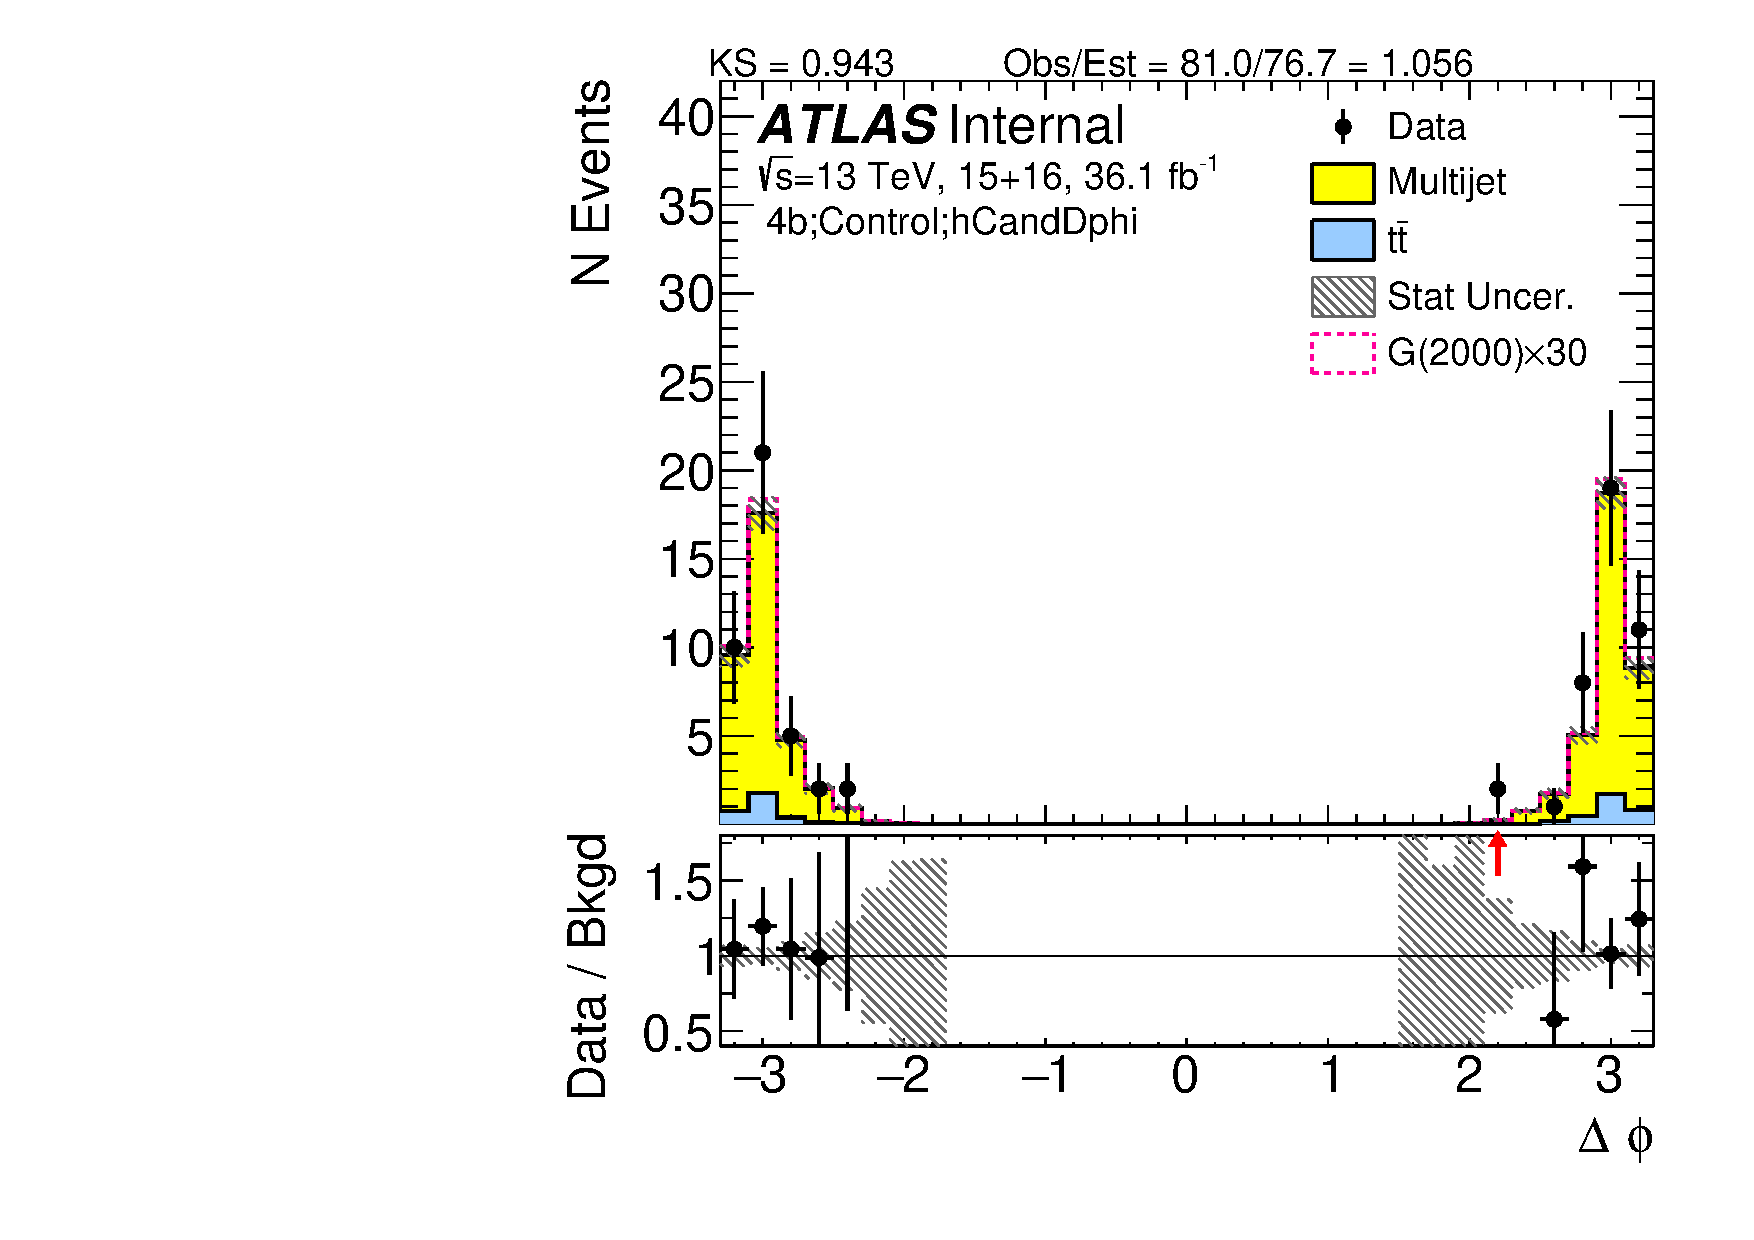
\includegraphics[width=0.32\textwidth,angle=-90]{figures/boosted/Control/b77_FourTag_Control_hCandDphi.pdf}
  \caption{Kinematics of the large-\R jet system in data and prediction in the control region after requiring 4 $b$-tags.  }
  \label{fig:boosted-4b-control-ak10-system}
\end{center}
\end{figure*}

\clearpage

\begin{figure*}[htbp!]
\begin{center}
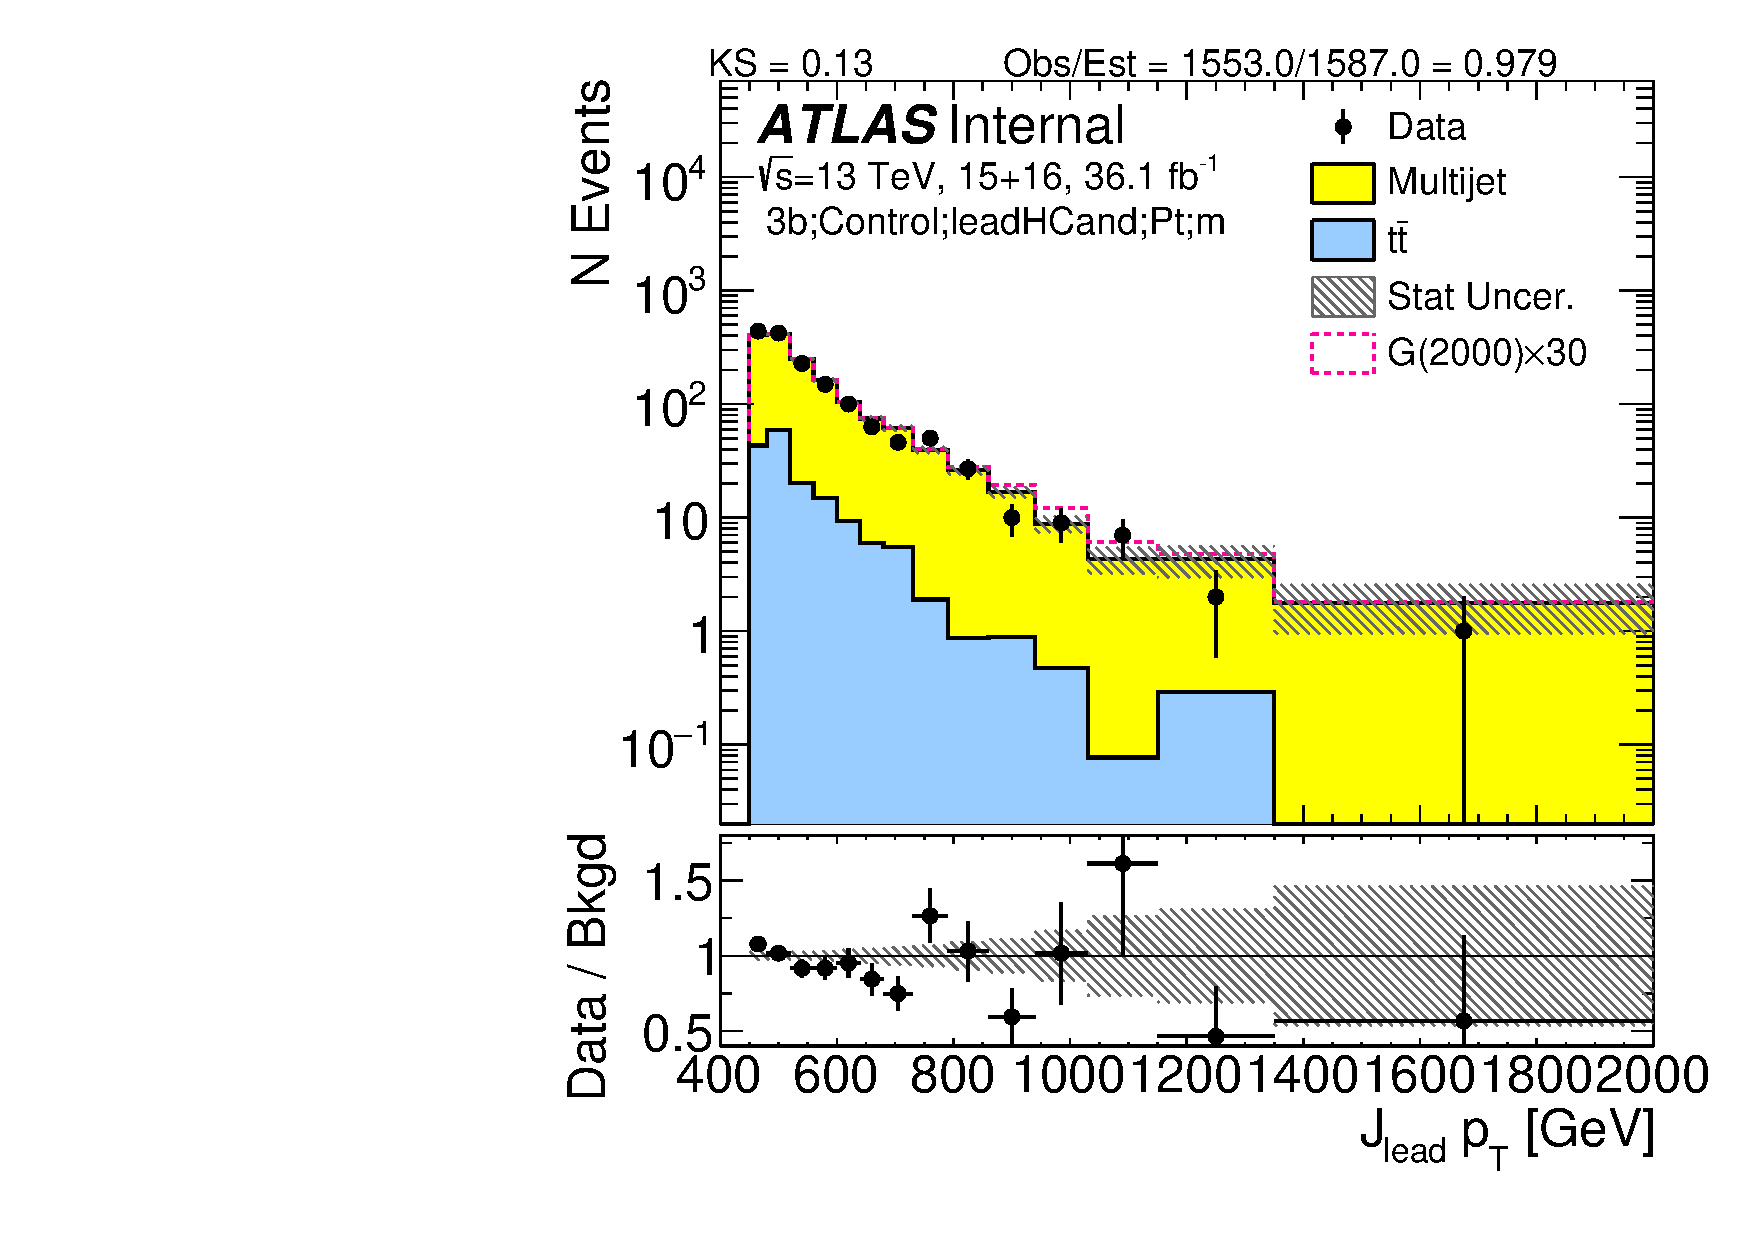
\includegraphics[width=0.32\textwidth,angle=-90]{figures/boosted/Control/b77_ThreeTag_Control_leadHCand_Pt_m_1.pdf}
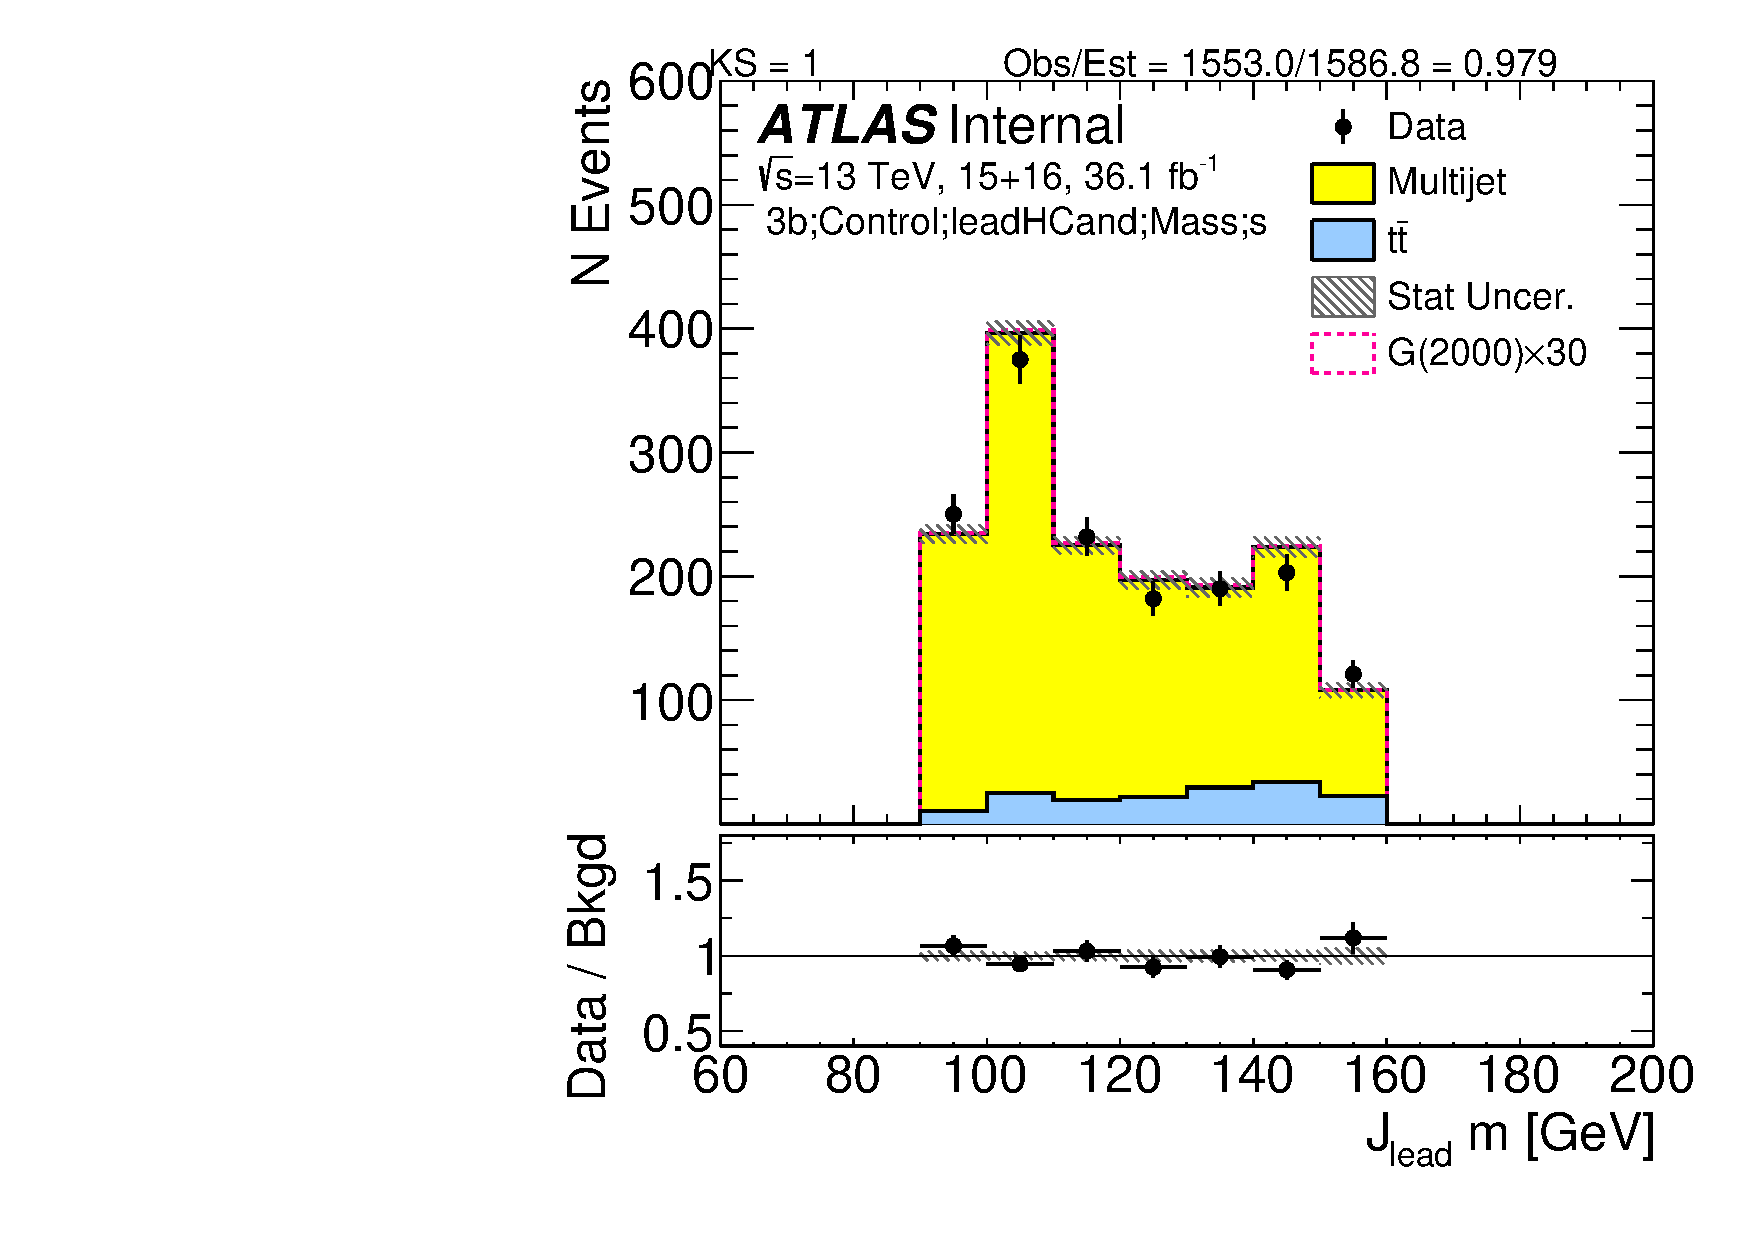
\includegraphics[width=0.32\textwidth,angle=-90]{figures/boosted/Control/b77_ThreeTag_Control_leadHCand_Mass_s.pdf}\\
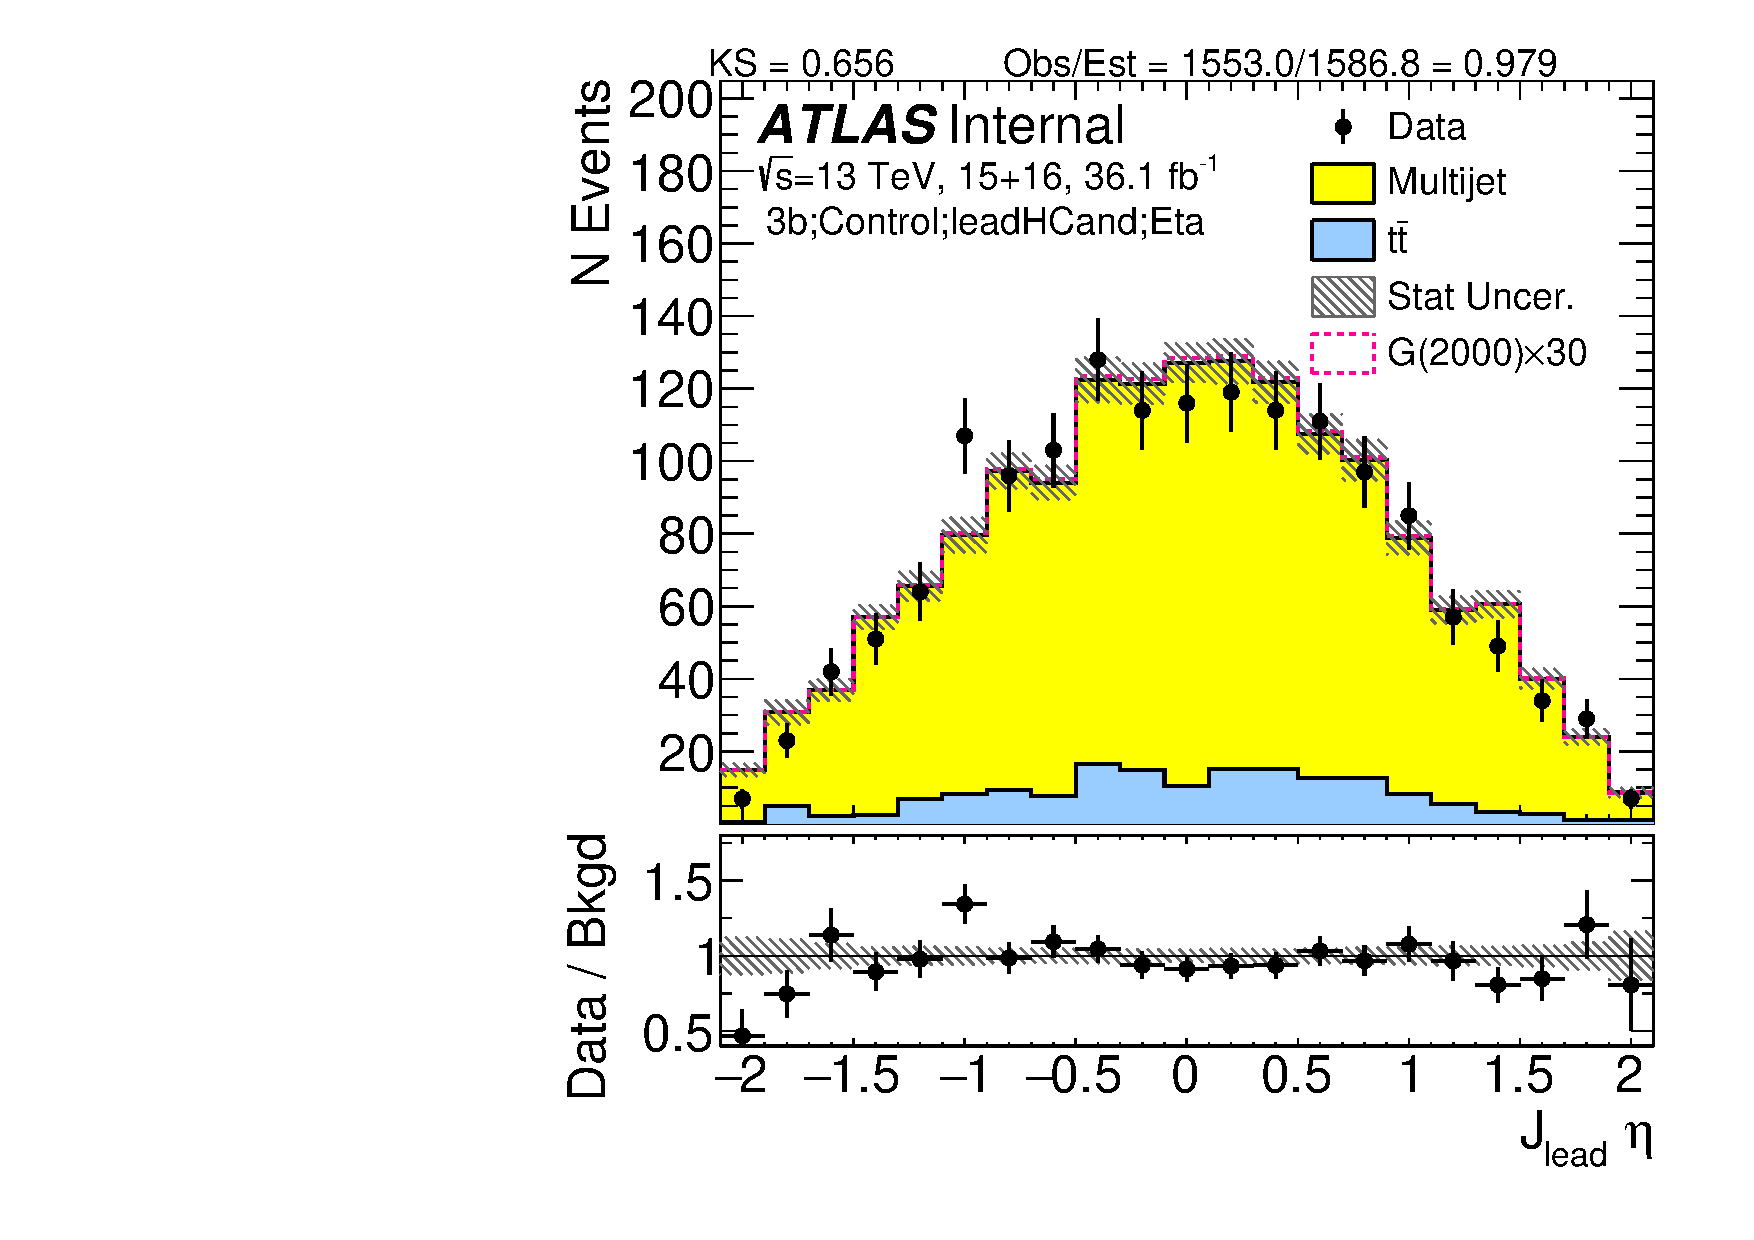
\includegraphics[width=0.32\textwidth,angle=-90]{figures/boosted/Control/b77_ThreeTag_Control_leadHCand_Eta.pdf}
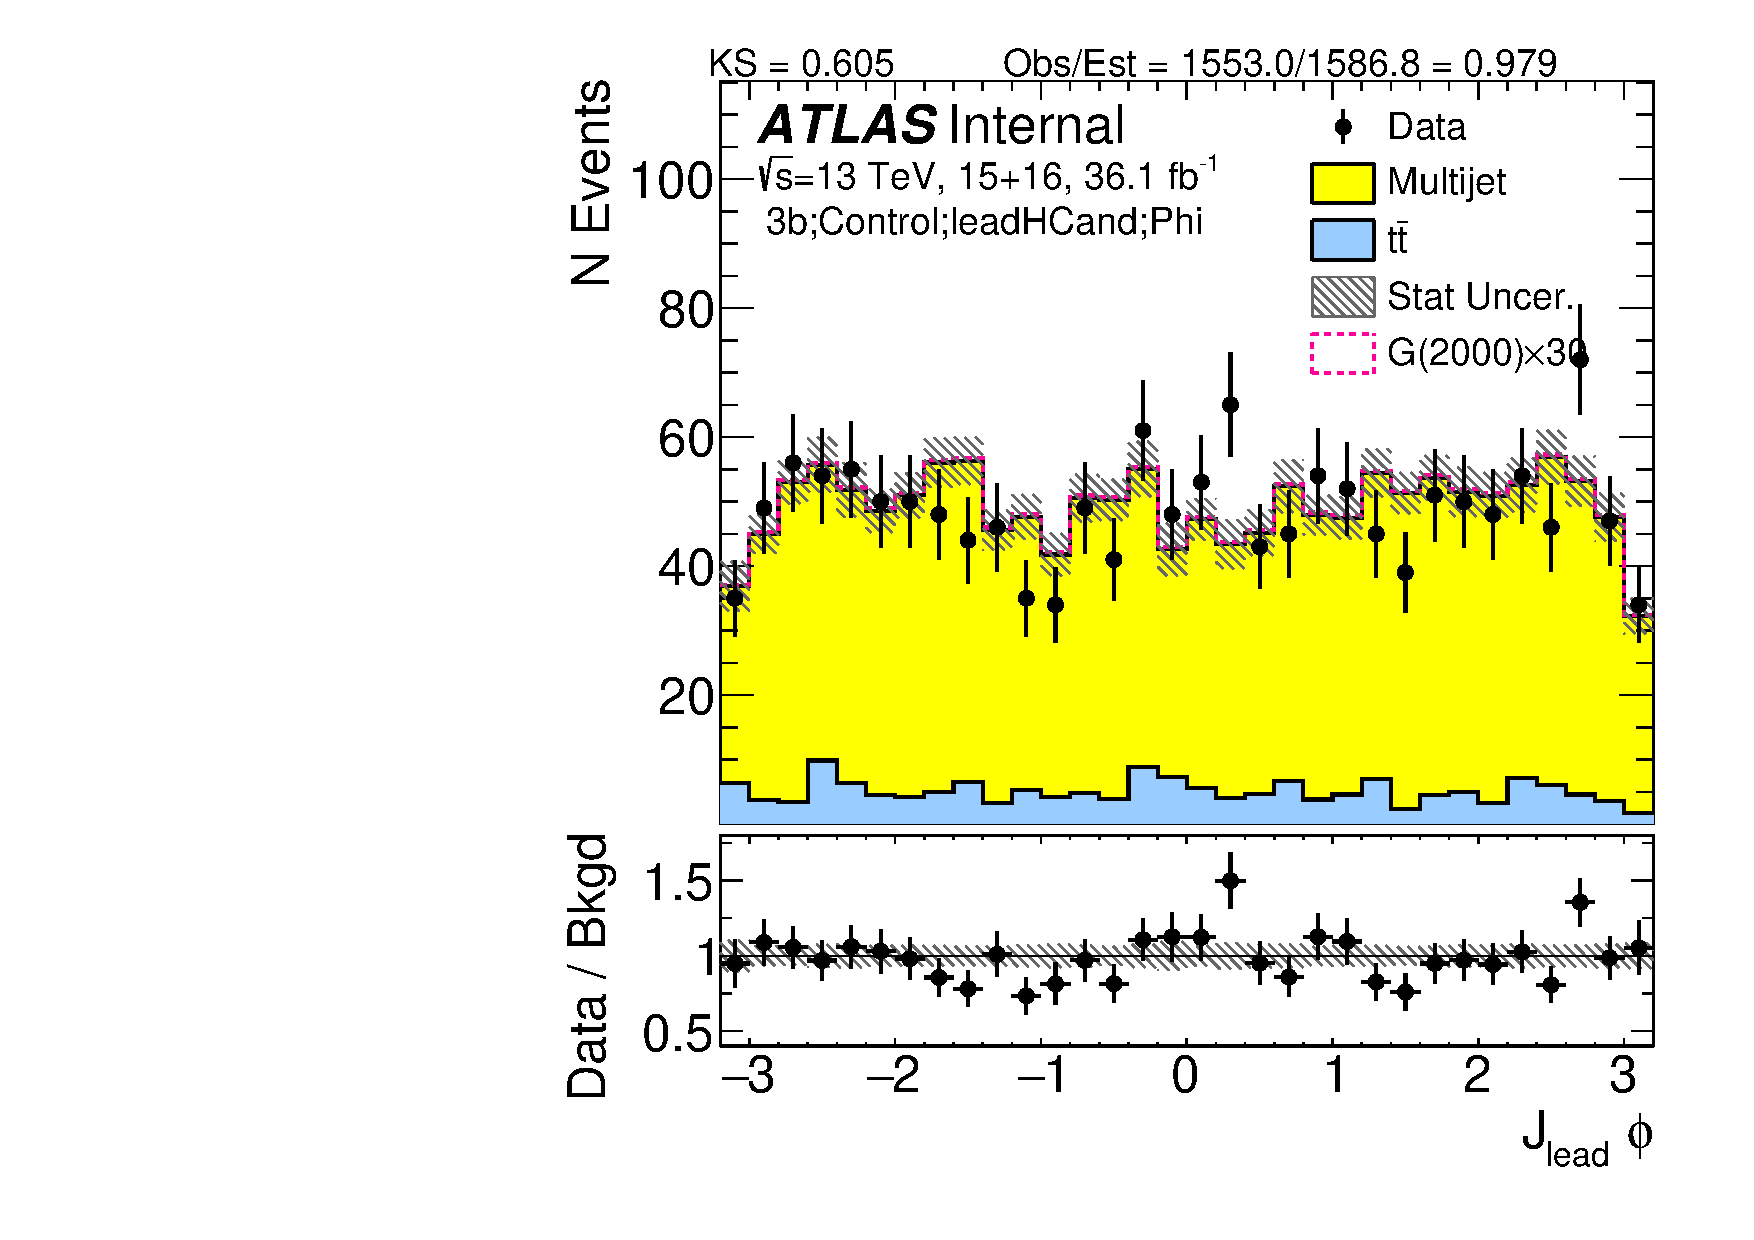
\includegraphics[width=0.32\textwidth,angle=-90]{figures/boosted/Control/b77_ThreeTag_Control_leadHCand_Phi.pdf}
  \caption{Kinematics of the lead large-\R jet in data and prediction in the control region after requiring 3 $b$-tags. }
  \label{fig:boosted-3b-control-ak10-lead}
\end{center}
\end{figure*}

\begin{figure*}[htbp!]
\begin{center}
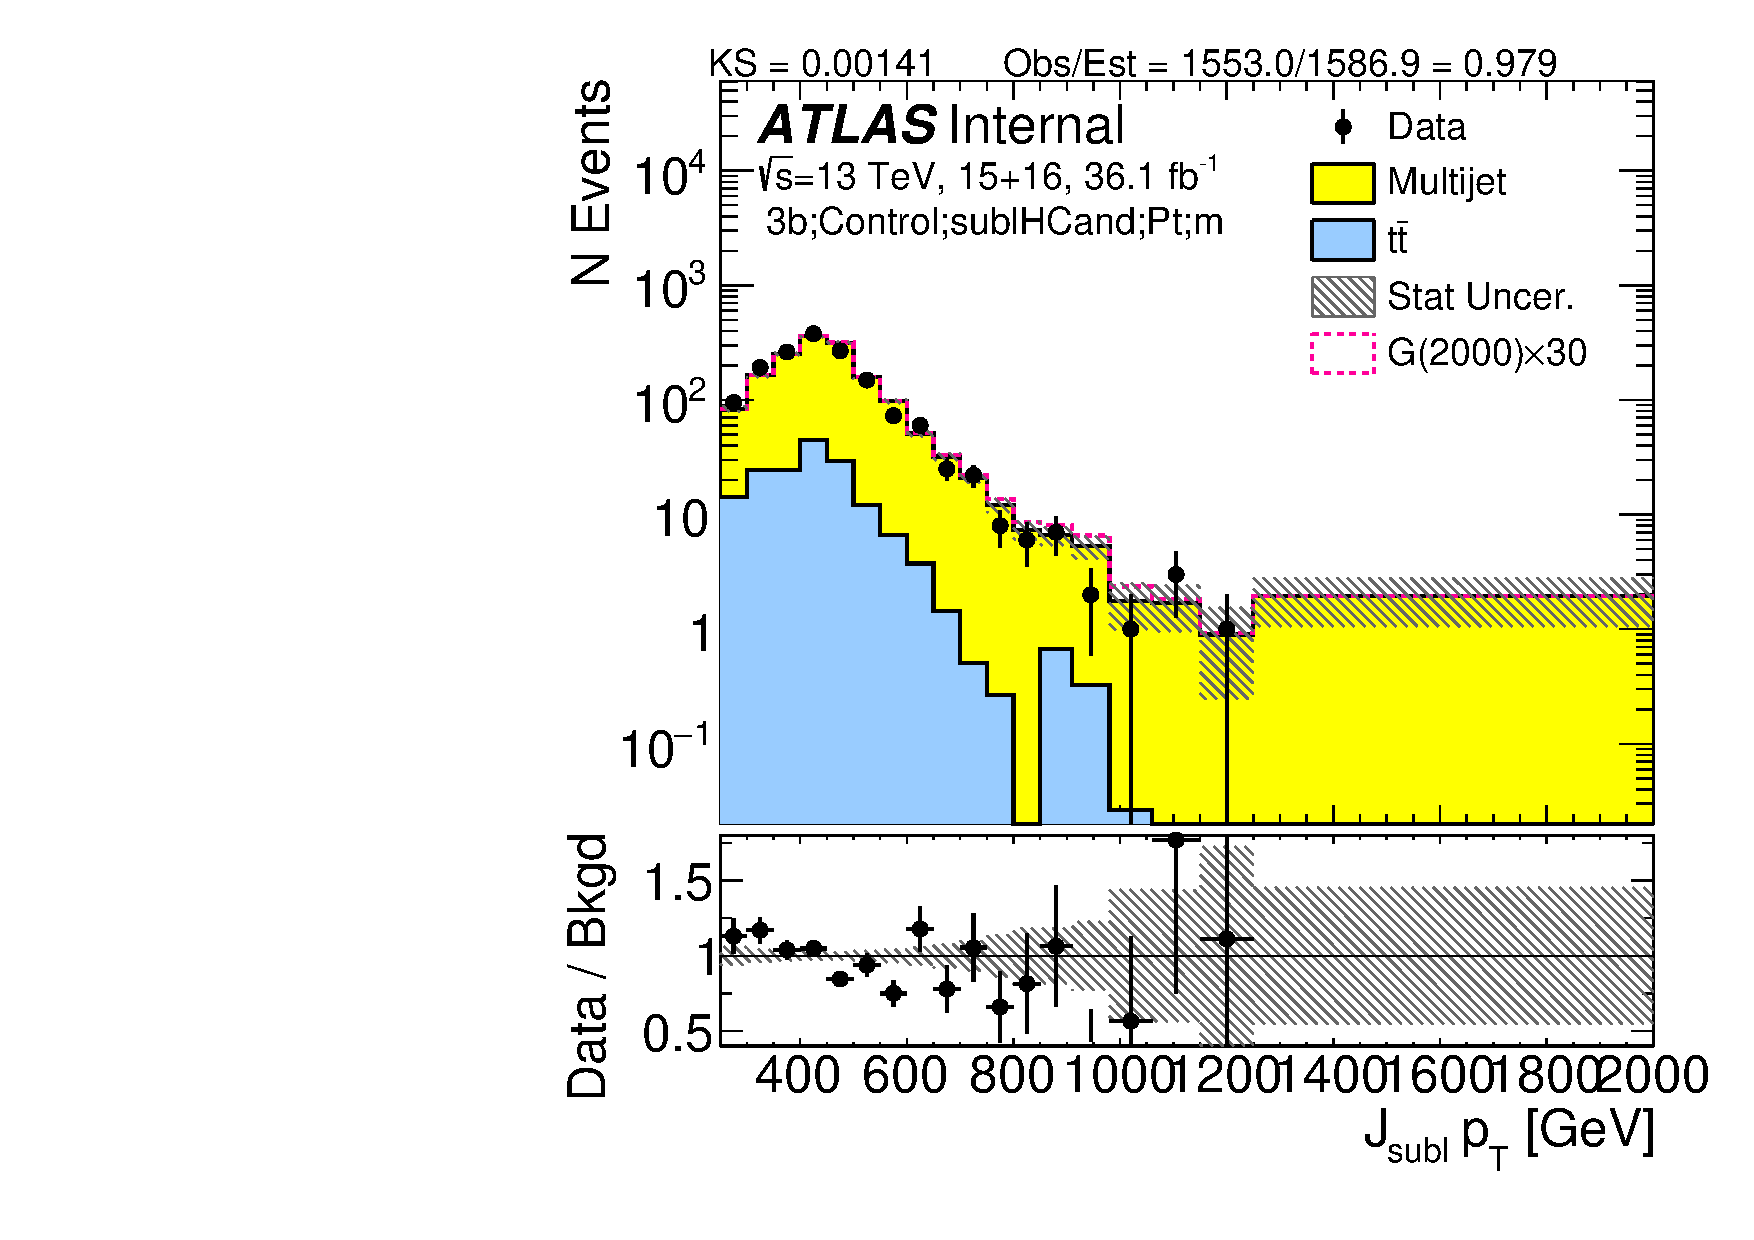
\includegraphics[width=0.32\textwidth,angle=-90]{figures/boosted/Control/b77_ThreeTag_Control_sublHCand_Pt_m_1.pdf}
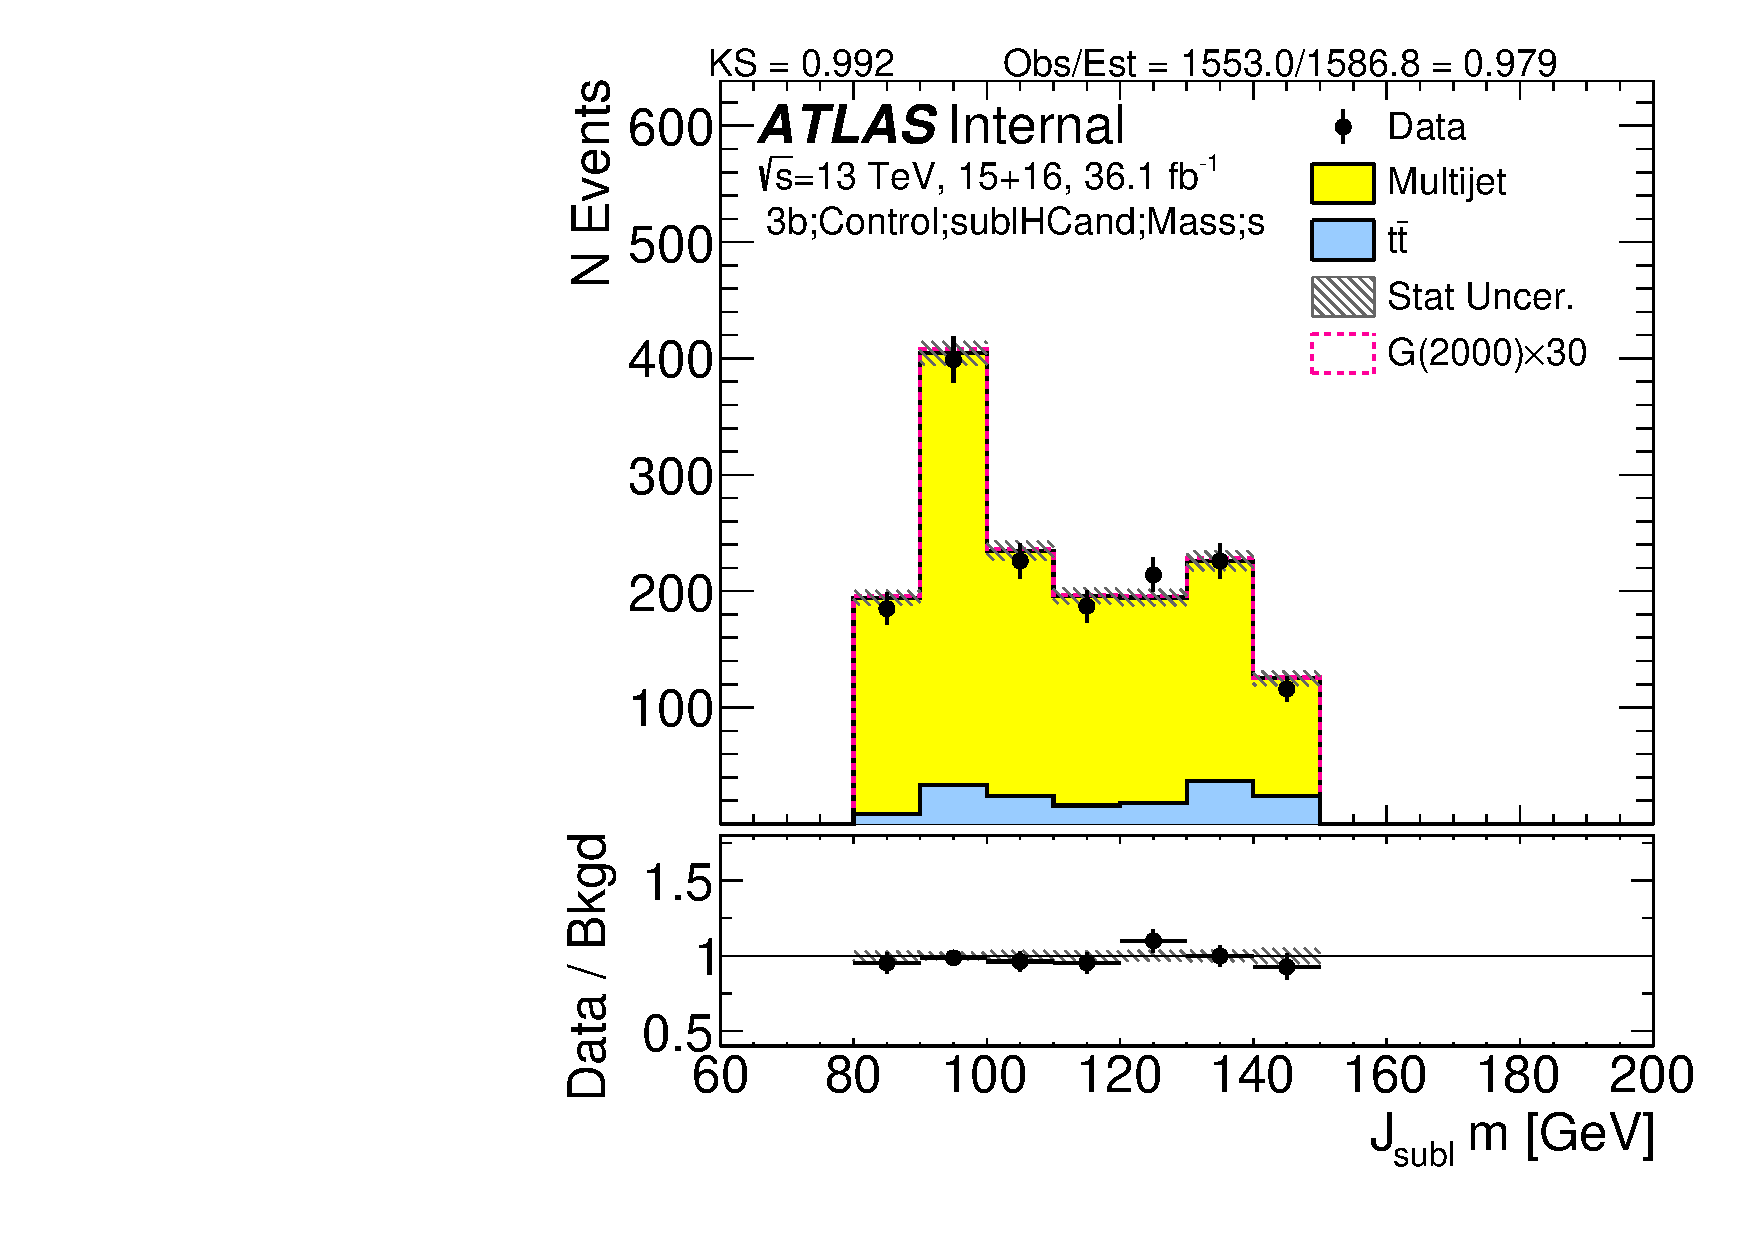
\includegraphics[width=0.32\textwidth,angle=-90]{figures/boosted/Control/b77_ThreeTag_Control_sublHCand_Mass_s.pdf}\\
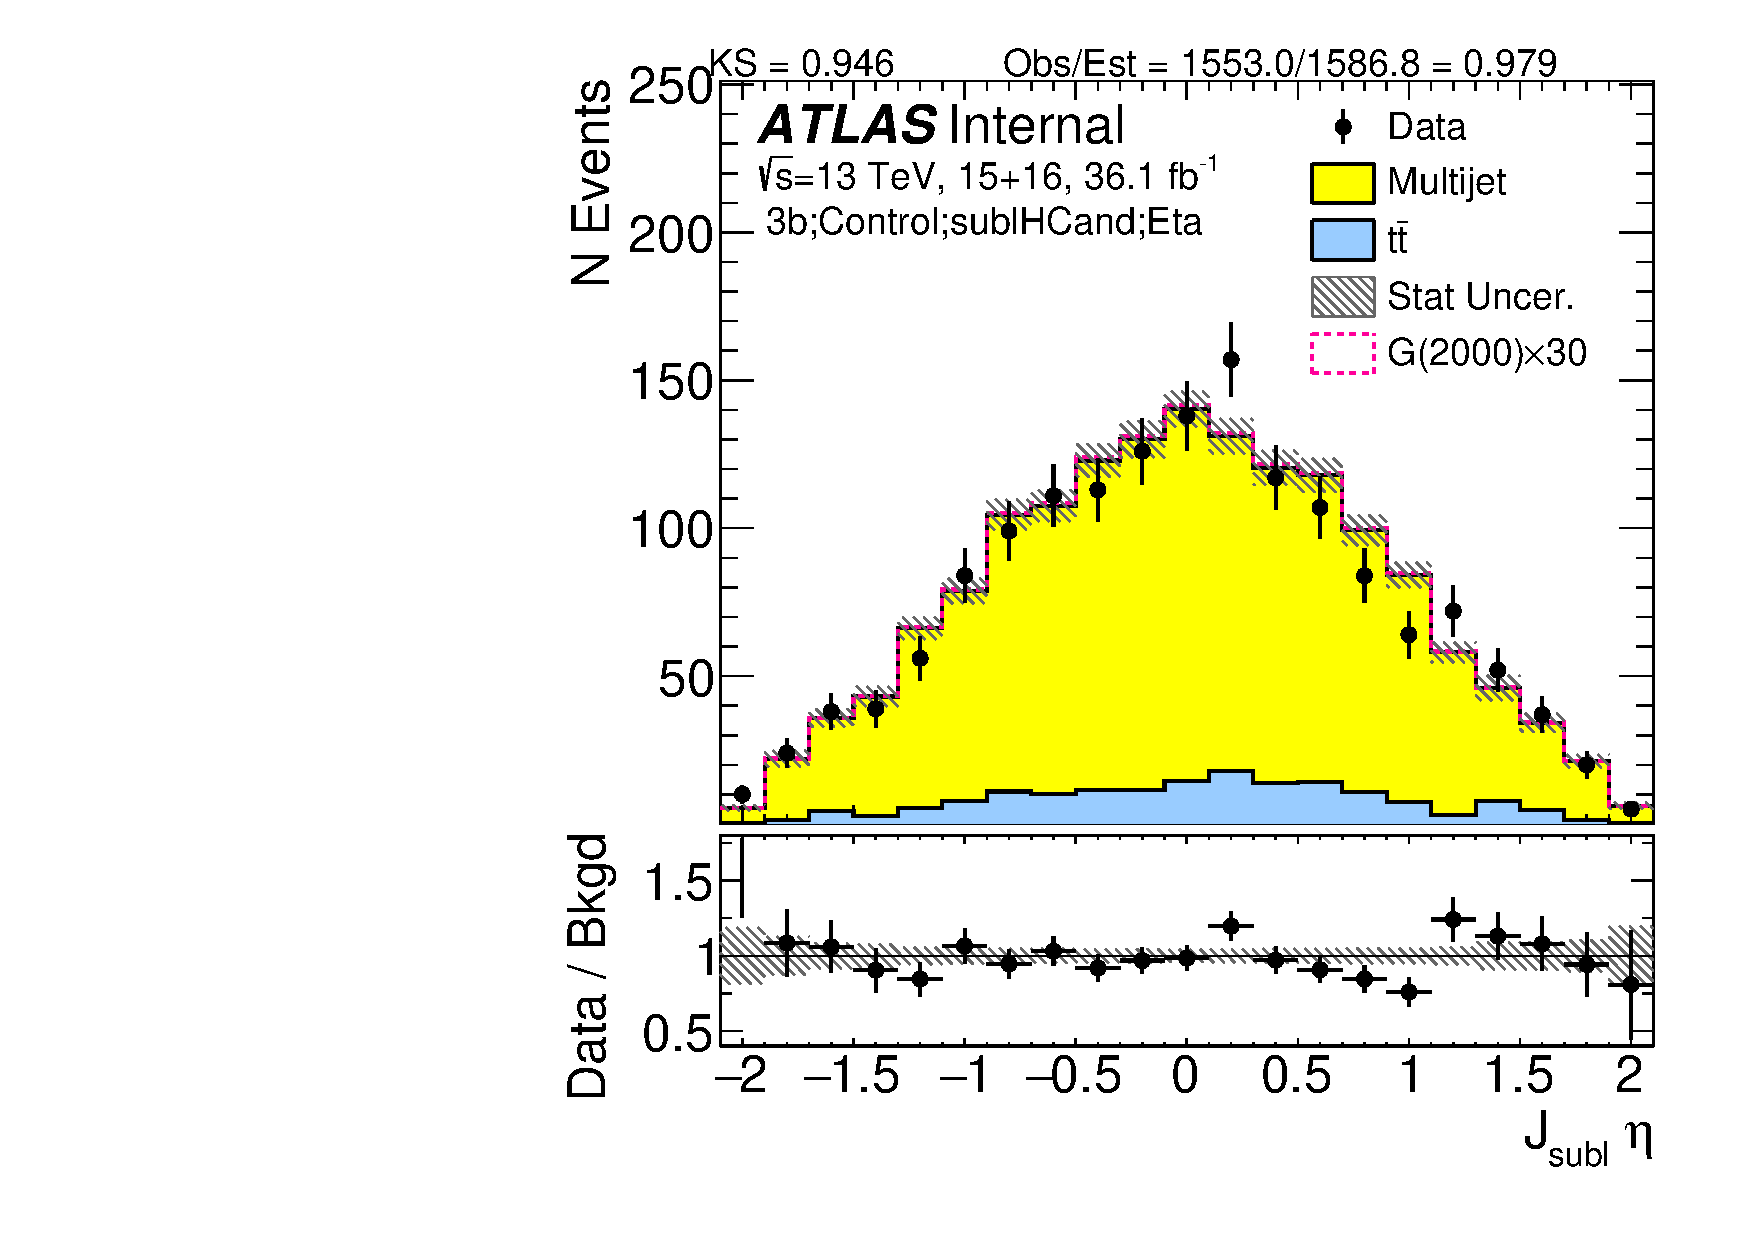
\includegraphics[width=0.32\textwidth,angle=-90]{figures/boosted/Control/b77_ThreeTag_Control_sublHCand_Eta.pdf}
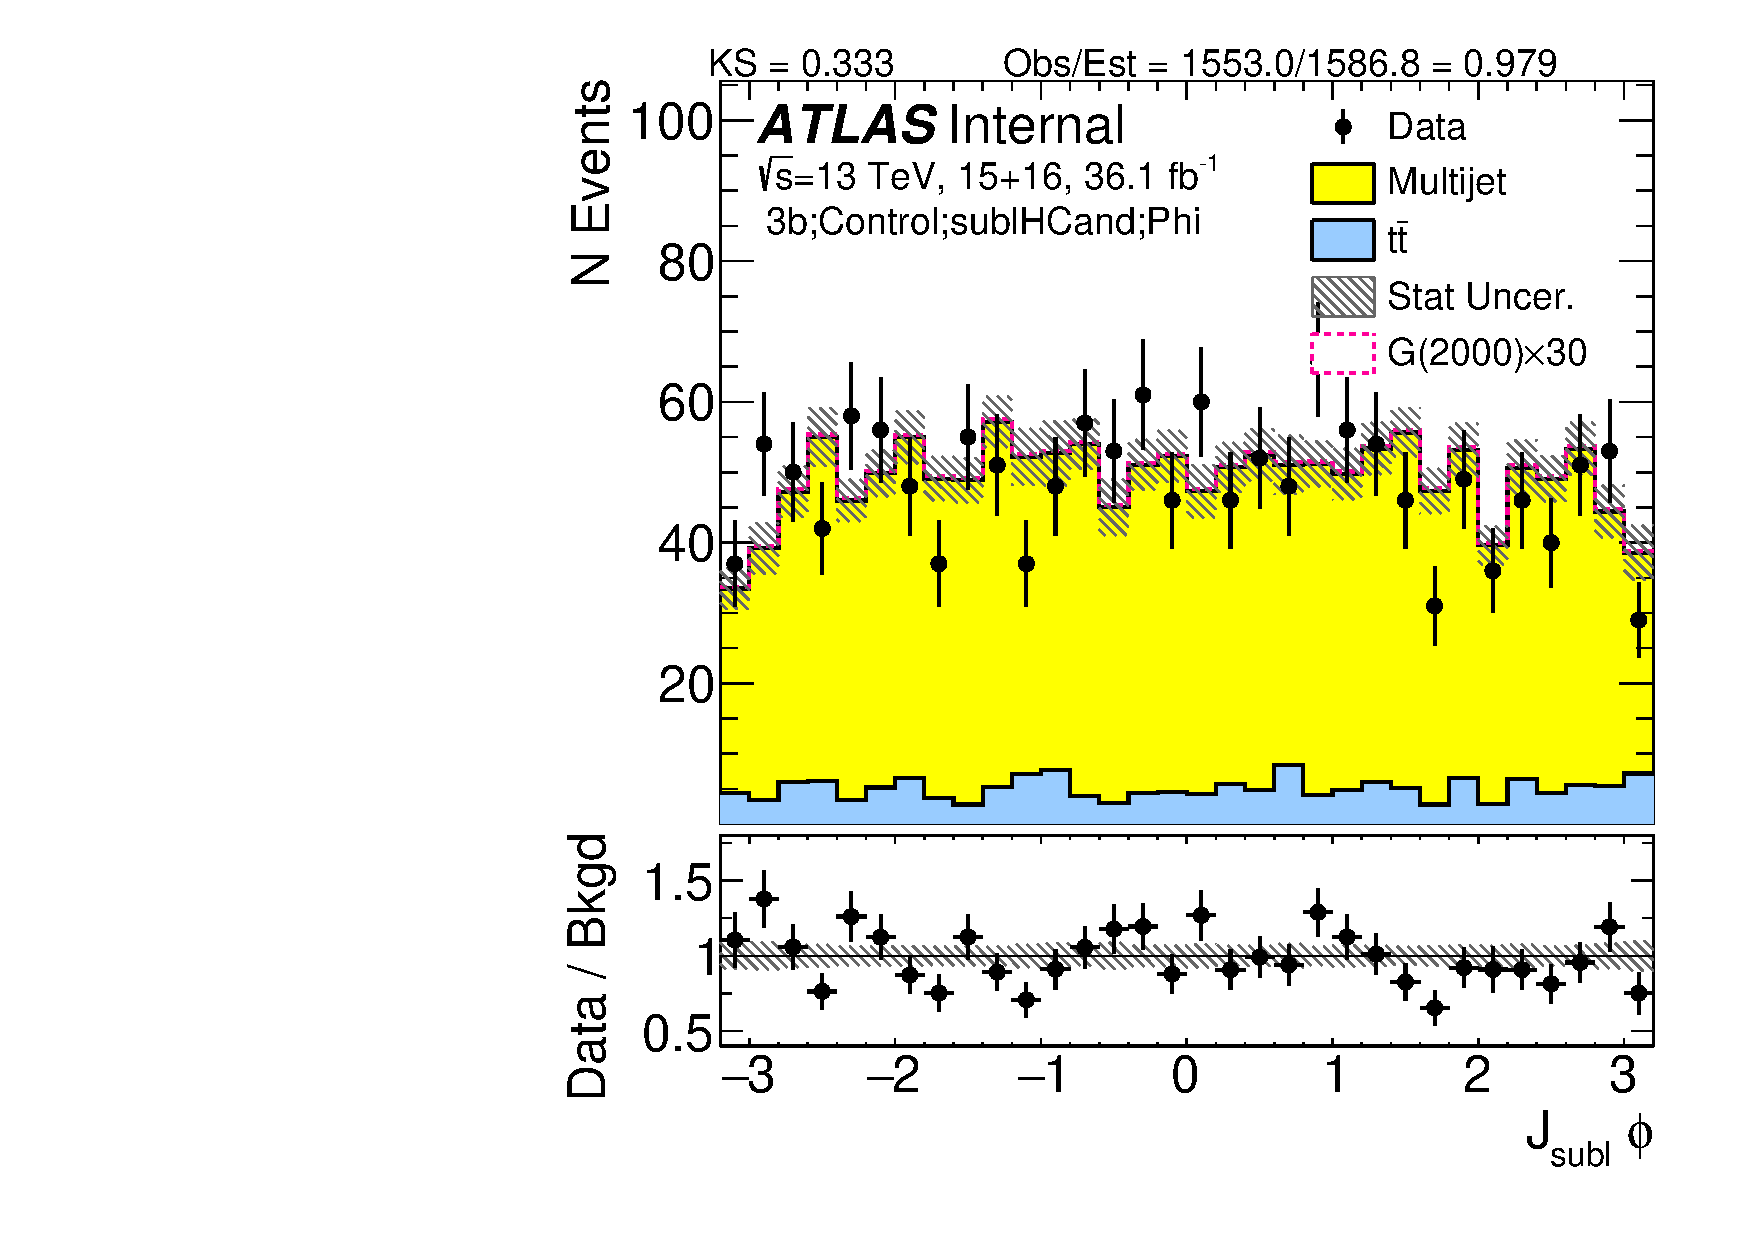
\includegraphics[width=0.32\textwidth,angle=-90]{figures/boosted/Control/b77_ThreeTag_Control_sublHCand_Phi.pdf}
  \caption{Kinematics of the sub-lead large-\R jet in data and prediction in the control region after requiring 3 $b$-tags. }
  \label{fig:boosted-3b-control-ak10-subl}
\end{center}
\end{figure*}

\begin{figure*}[htbp!]
\begin{center}
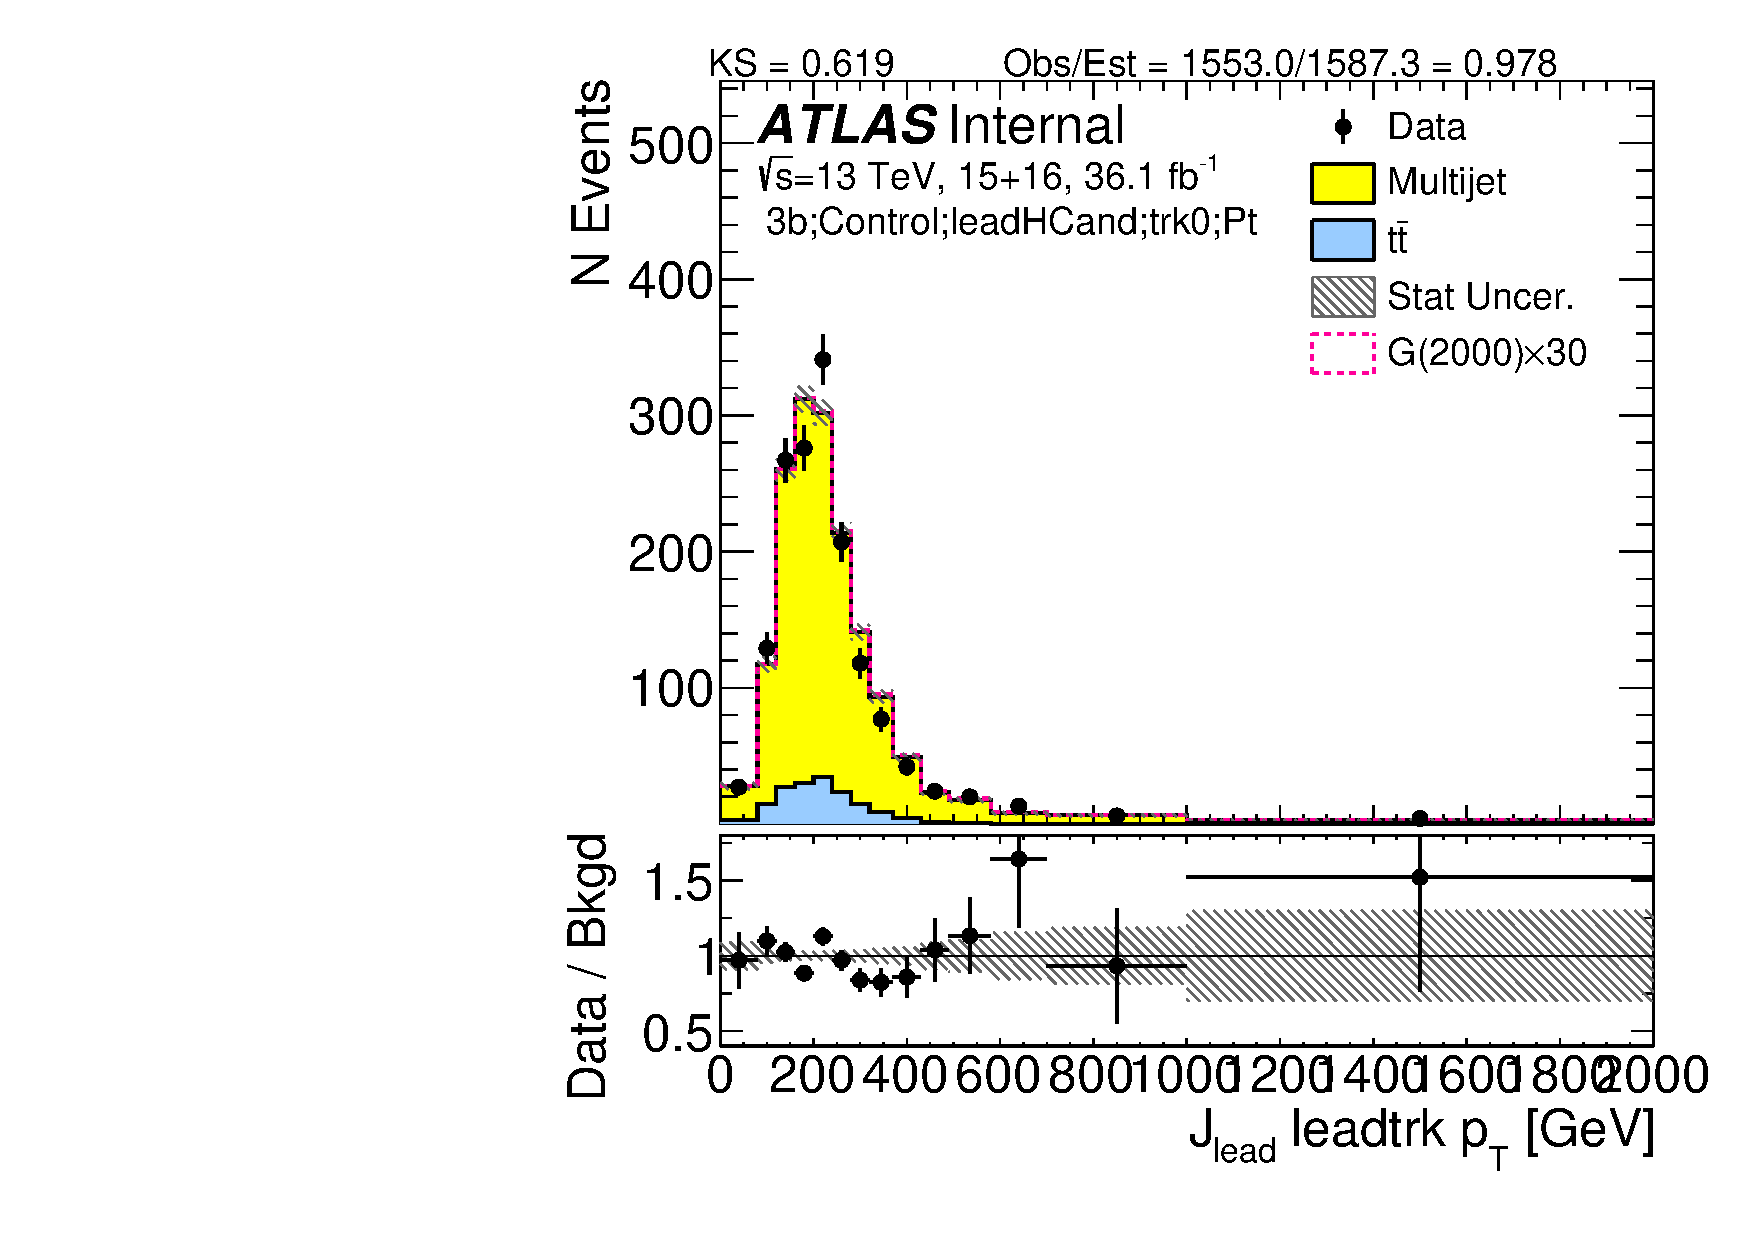
\includegraphics[width=0.32\textwidth,angle=-90]{figures/boosted/Control/b77_ThreeTag_Control_leadHCand_trk0_Pt.pdf}
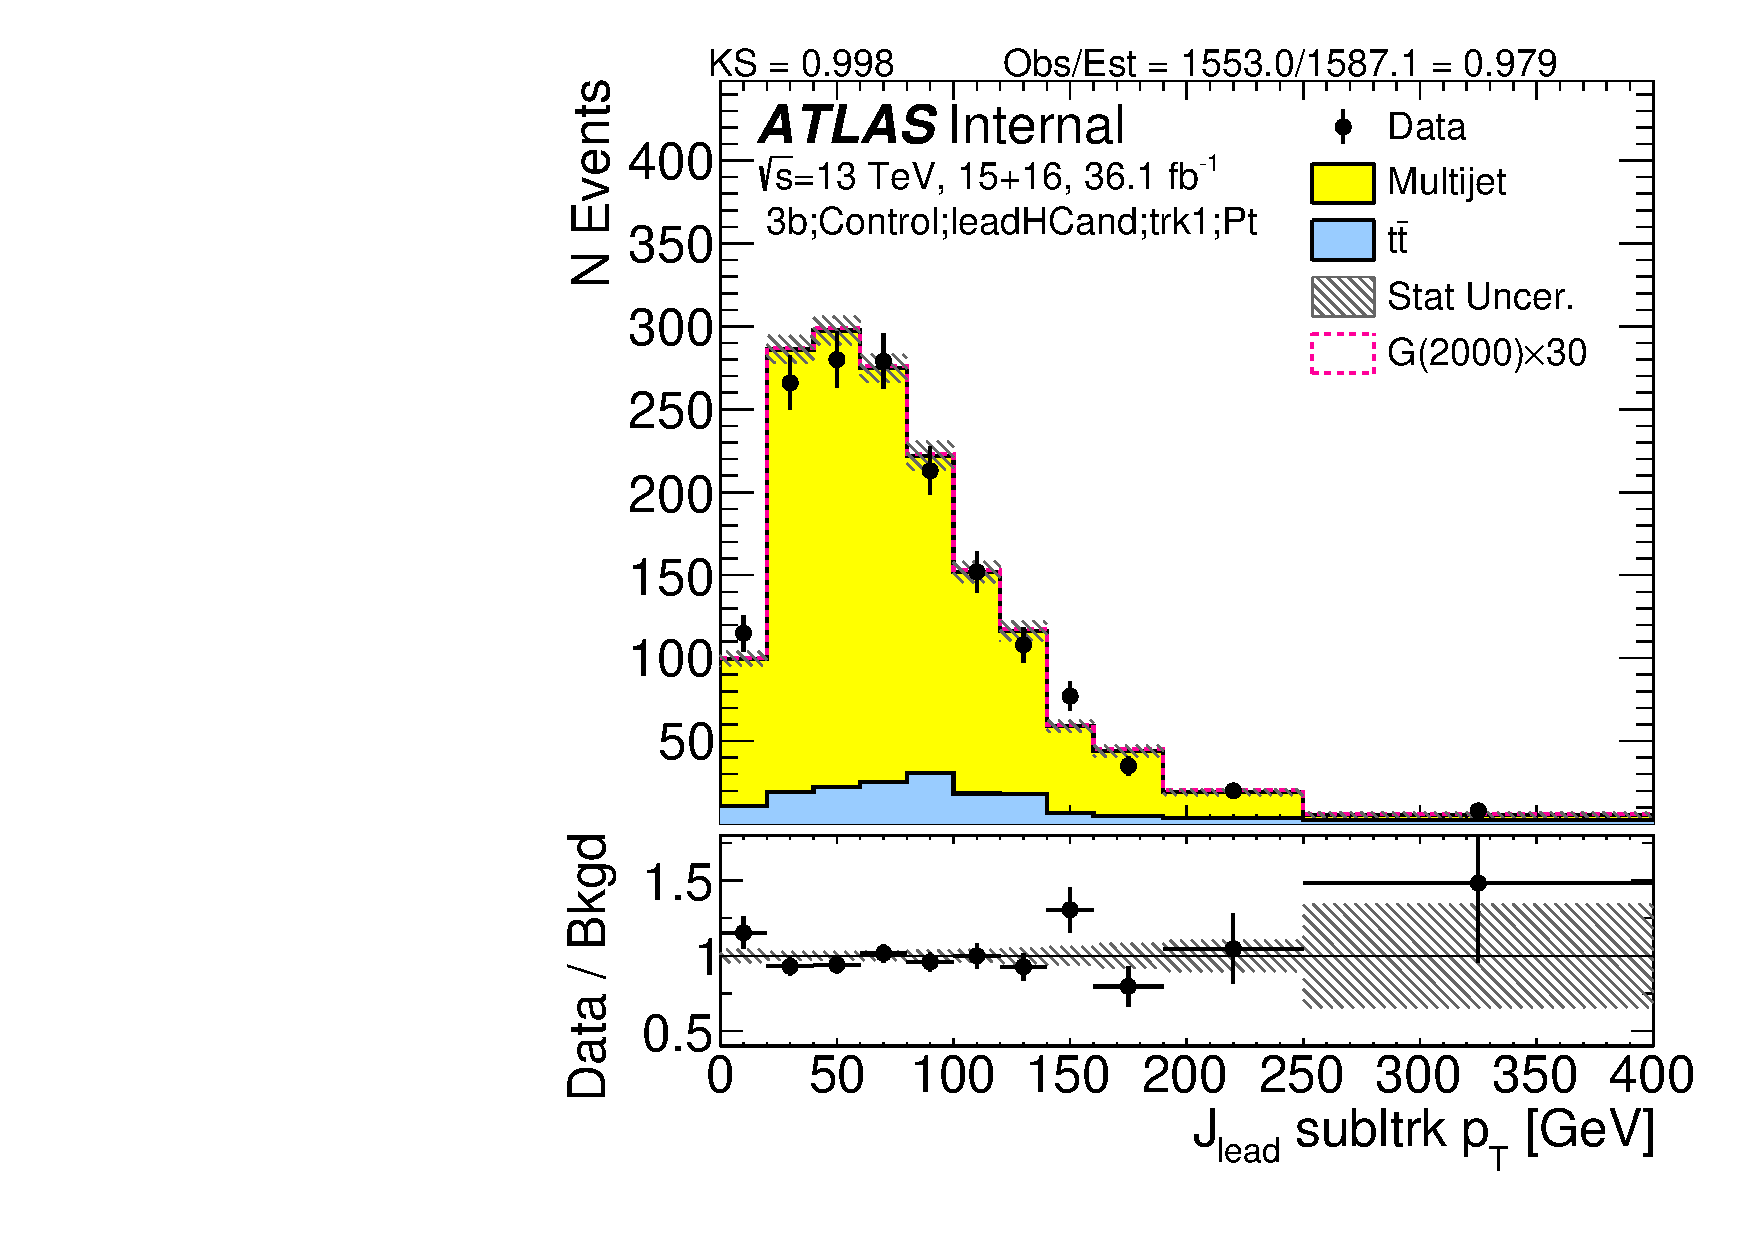
\includegraphics[width=0.32\textwidth,angle=-90]{figures/boosted/Control/b77_ThreeTag_Control_leadHCand_trk1_Pt.pdf}\\
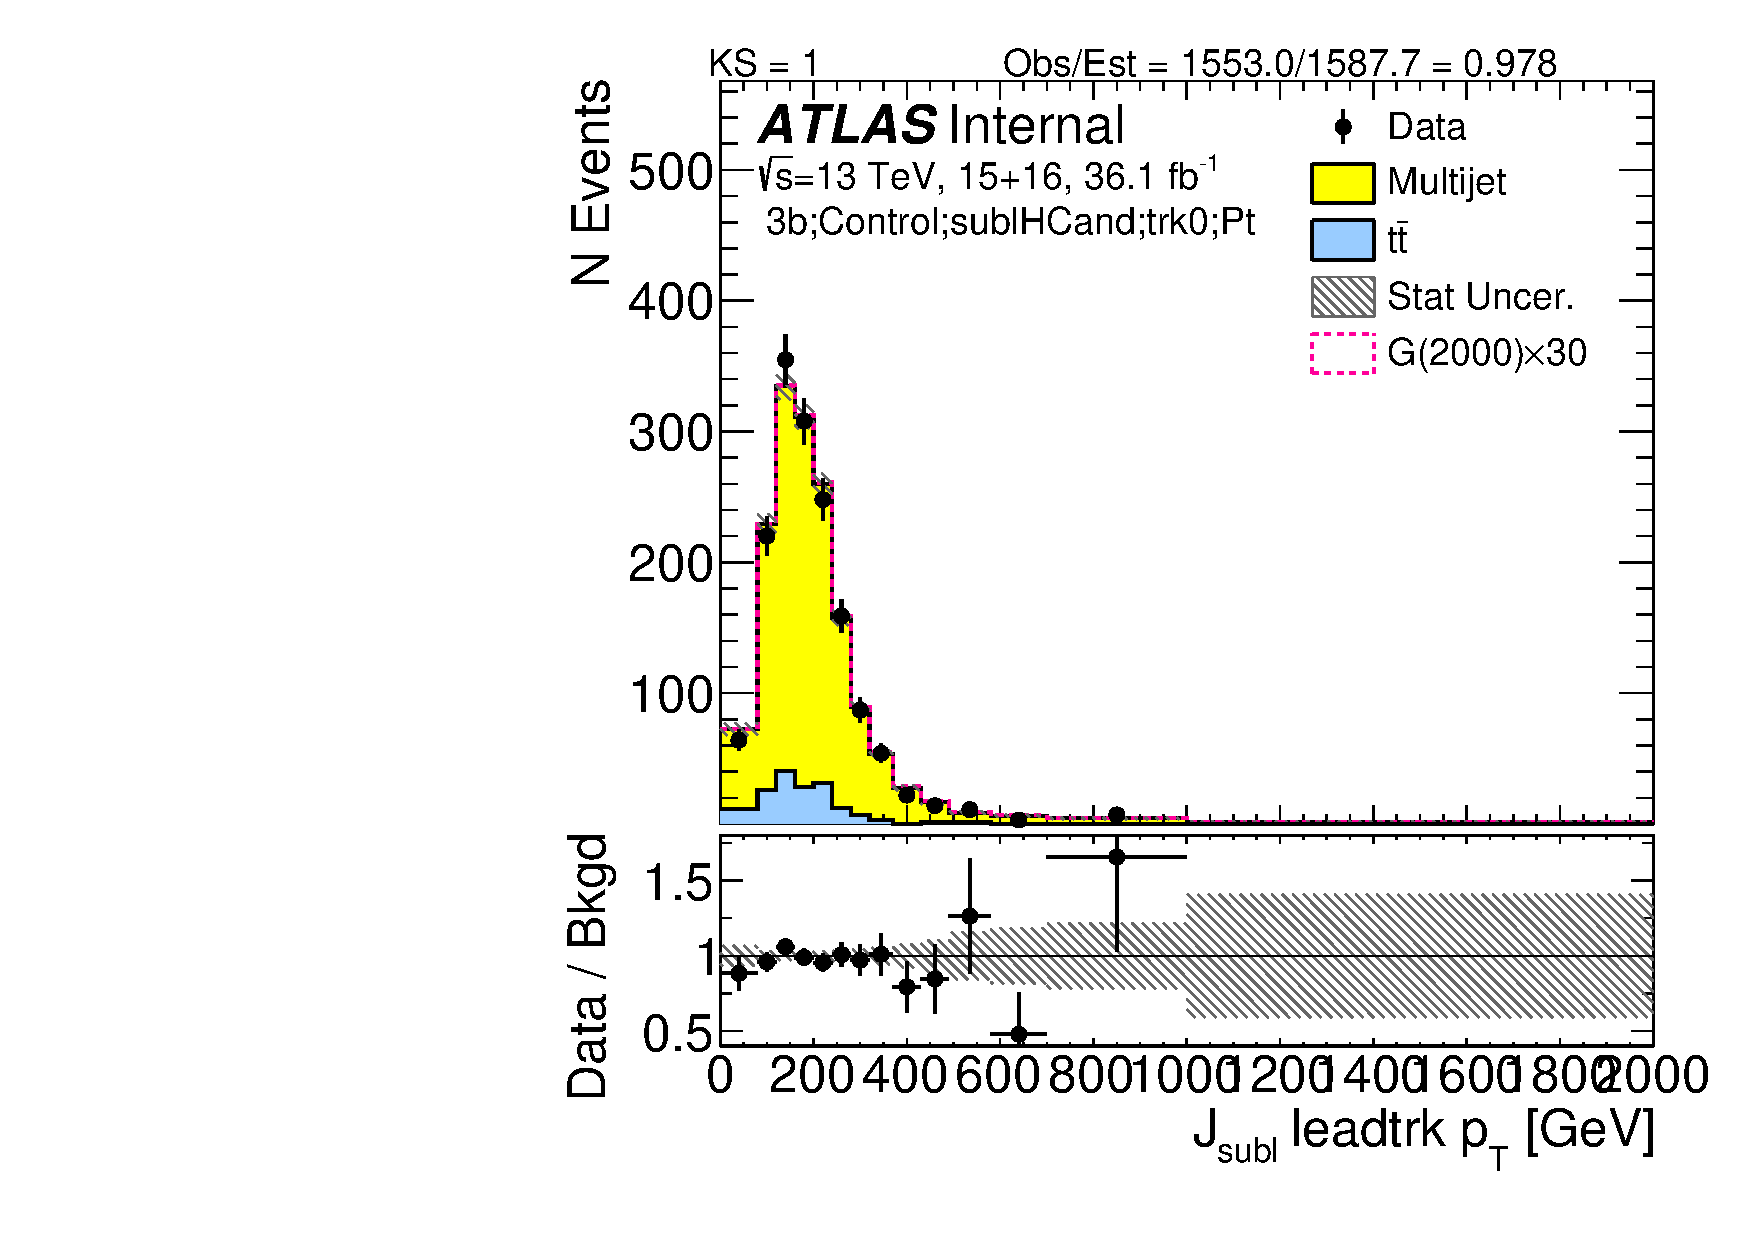
\includegraphics[width=0.32\textwidth,angle=-90]{figures/boosted/Control/b77_ThreeTag_Control_sublHCand_trk0_Pt.pdf}
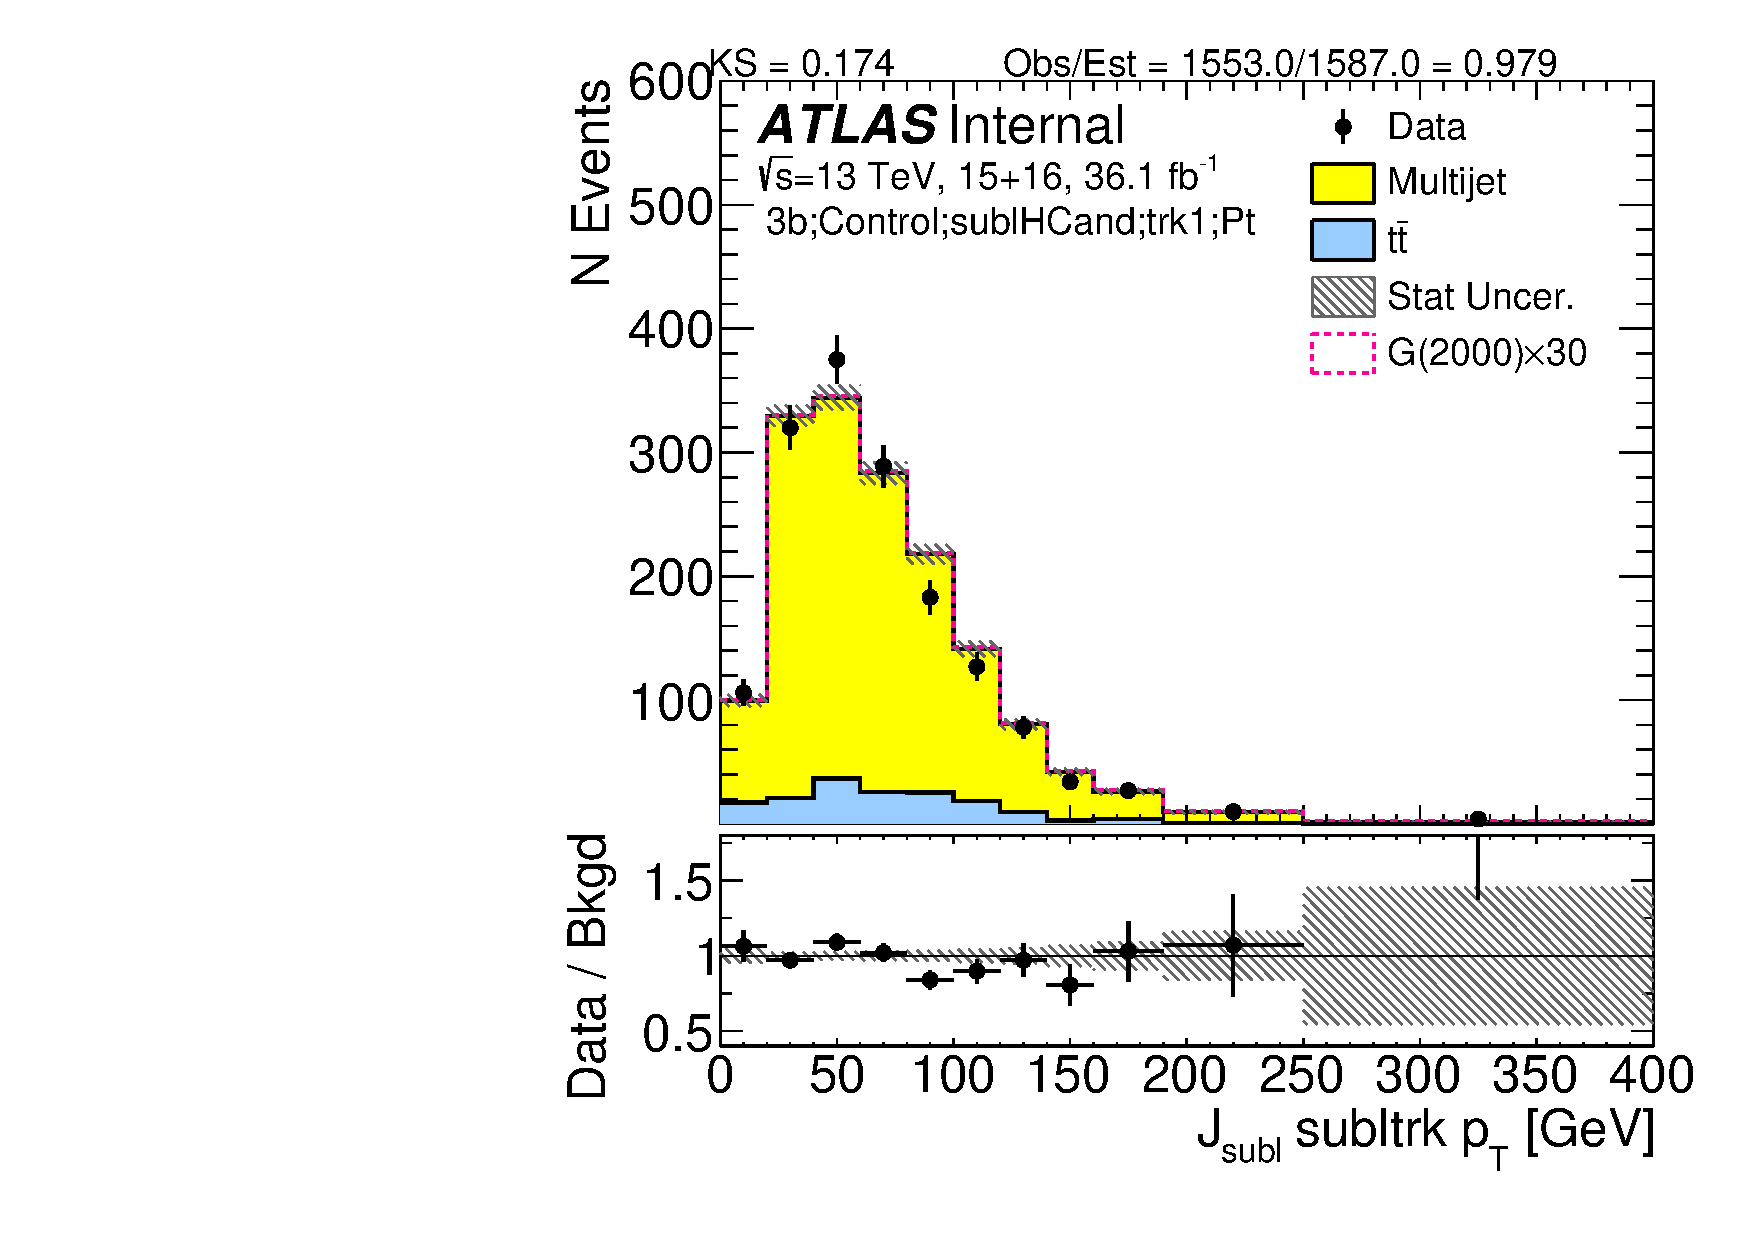
\includegraphics[width=0.32\textwidth,angle=-90]{figures/boosted/Control/b77_ThreeTag_Control_sublHCand_trk1_Pt.pdf}\\
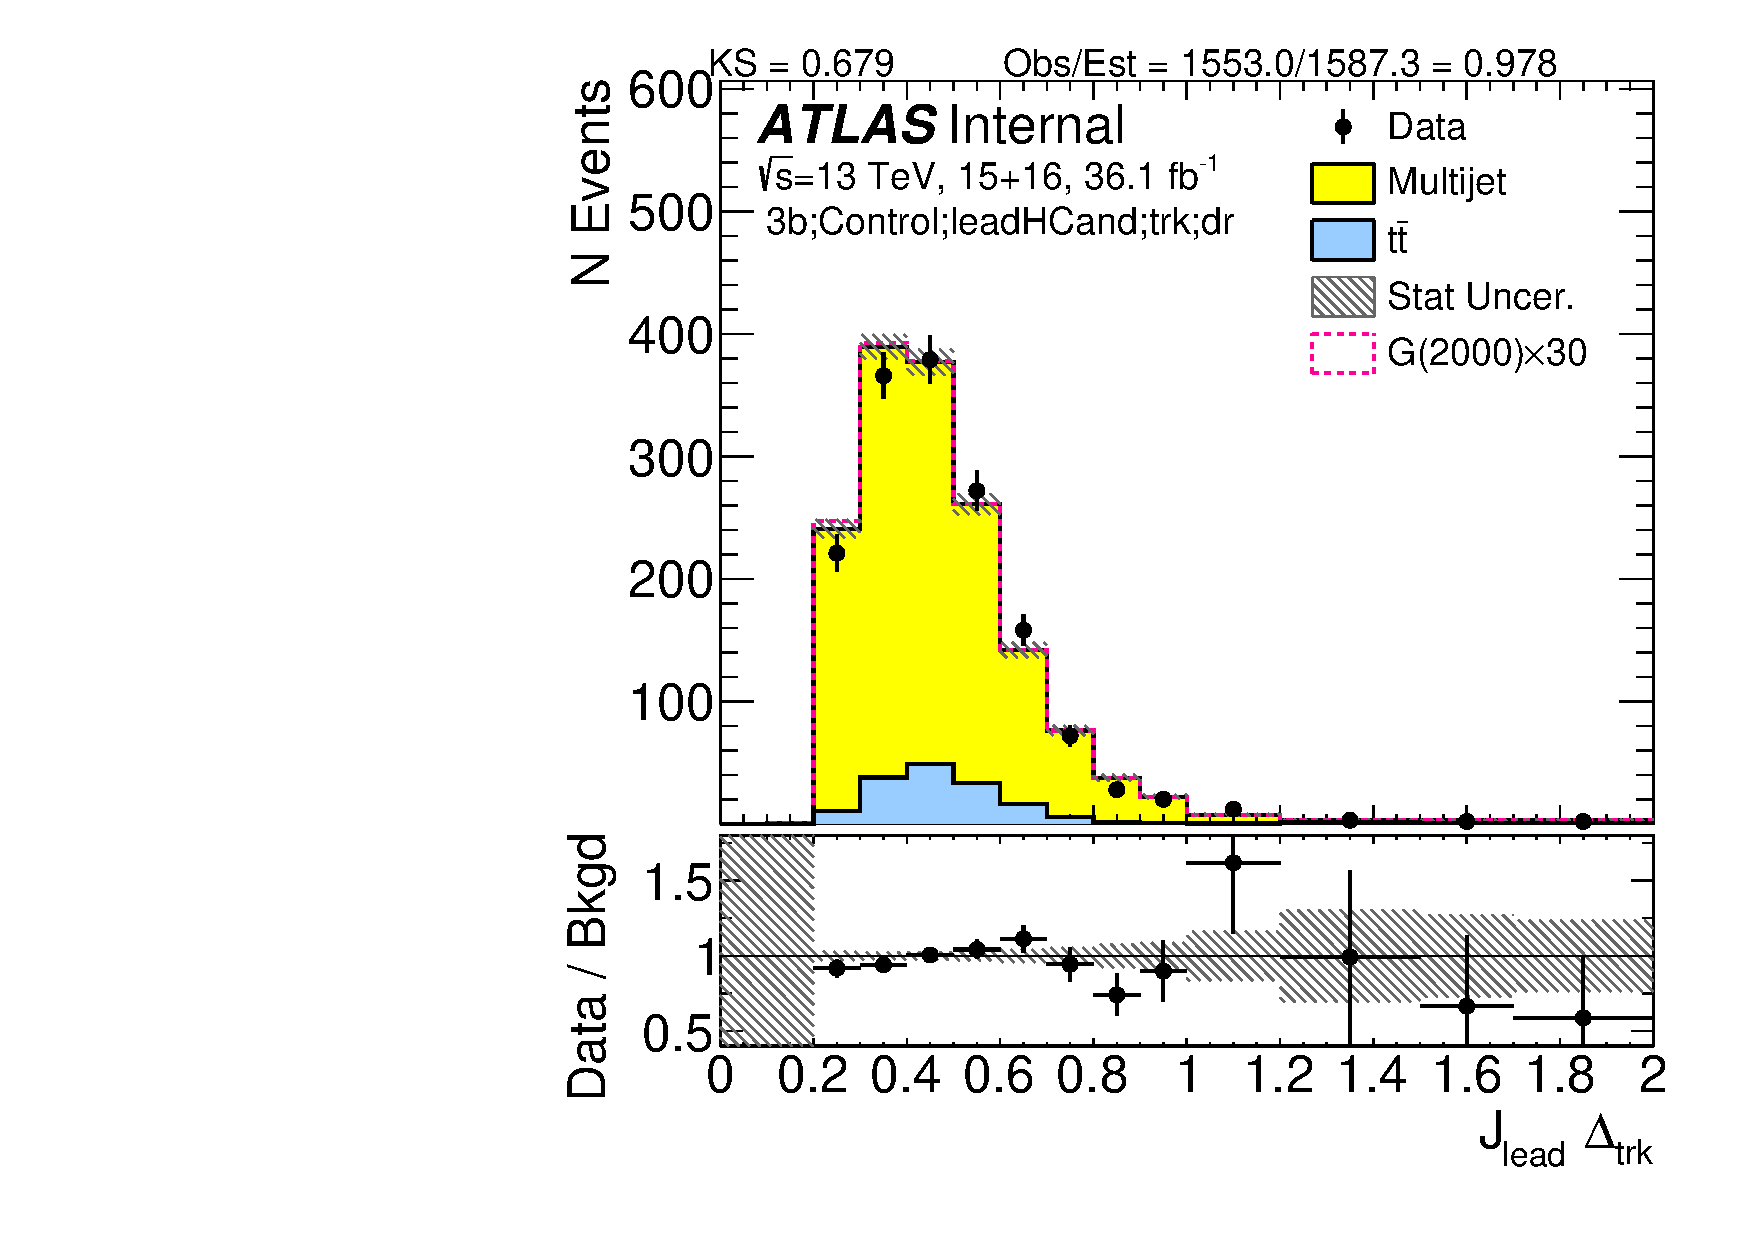
\includegraphics[width=0.32\textwidth,angle=-90]{figures/boosted/Control/b77_ThreeTag_Control_leadHCand_trk_dr.pdf}
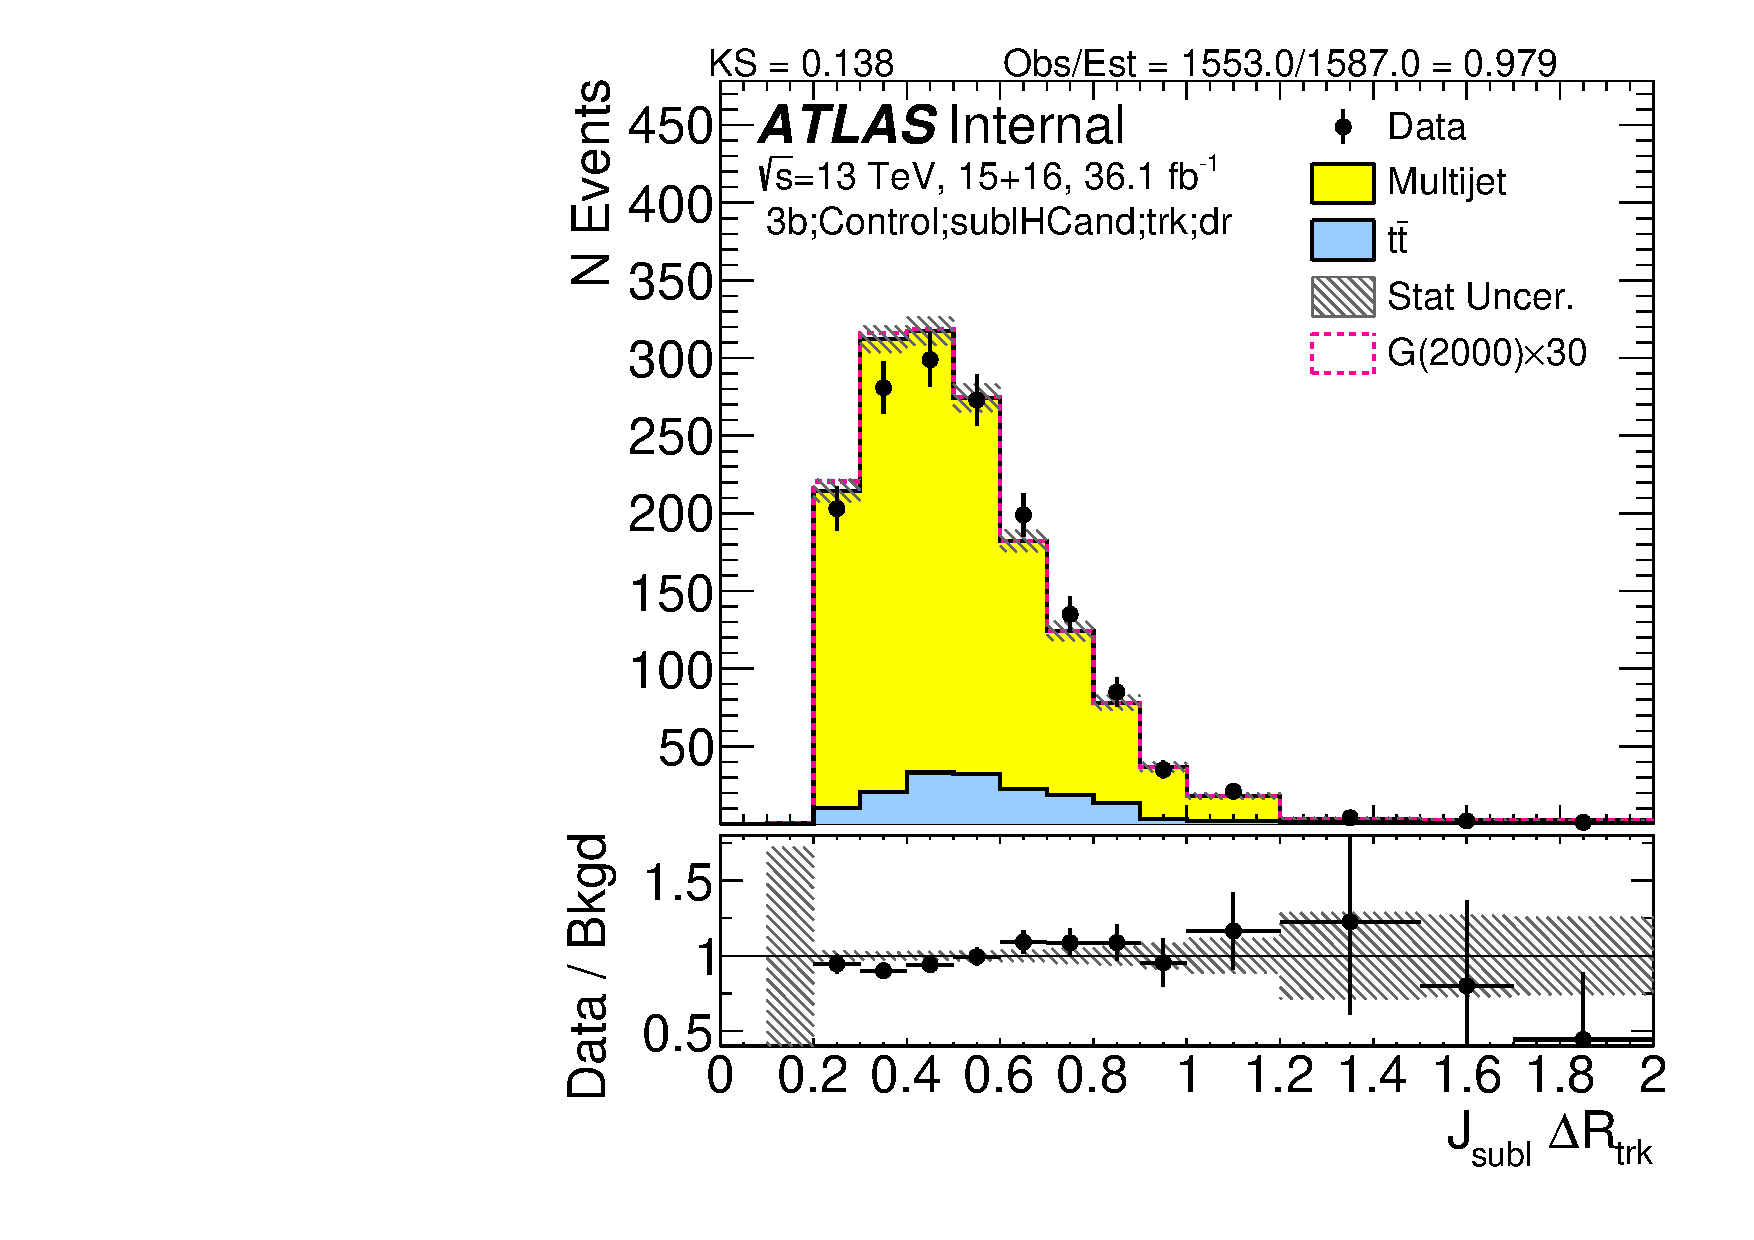
\includegraphics[width=0.32\textwidth,angle=-90]{figures/boosted/Control/b77_ThreeTag_Control_sublHCand_trk_dr.pdf}
  \caption{First two rows show the kinematics of the lead (left) and sub-lead (right) small-$R$ track jets associated to the lead (first-row) and sub-lead (second-row) large-\R jet in data and prediction in the control region after requiring 3 $b$-tags. Third row shows the $\Delta R$ between two leading small-$R$ track-jets associated to the leading (left) and sub-leading (right) large-\R jet.  }
  \label{fig:boosted-3b-control-ak2}
\end{center}
\end{figure*}


\begin{figure*}[htbp!]
\begin{center}
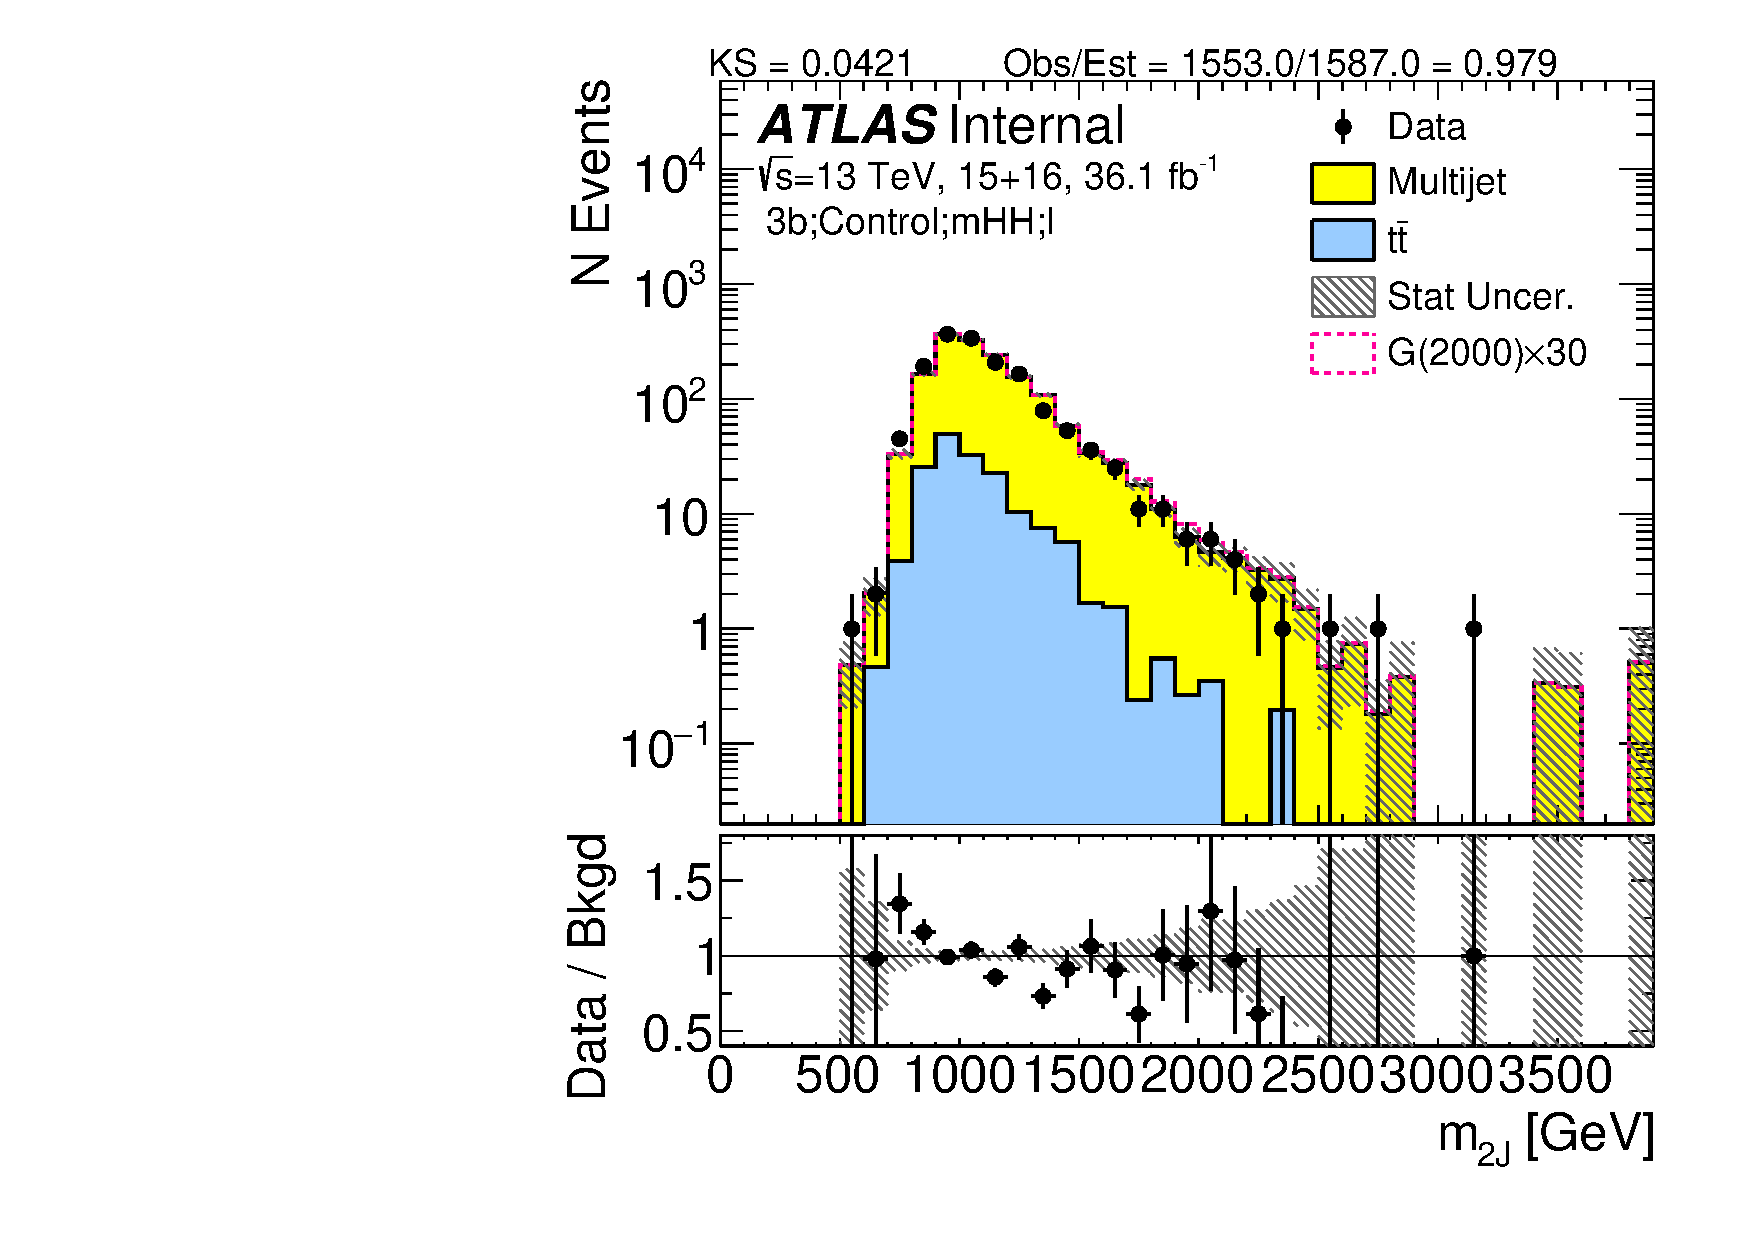
\includegraphics[width=0.32\textwidth,angle=-90]{figures/boosted/Control/b77_ThreeTag_Control_mHH_l_1.pdf}
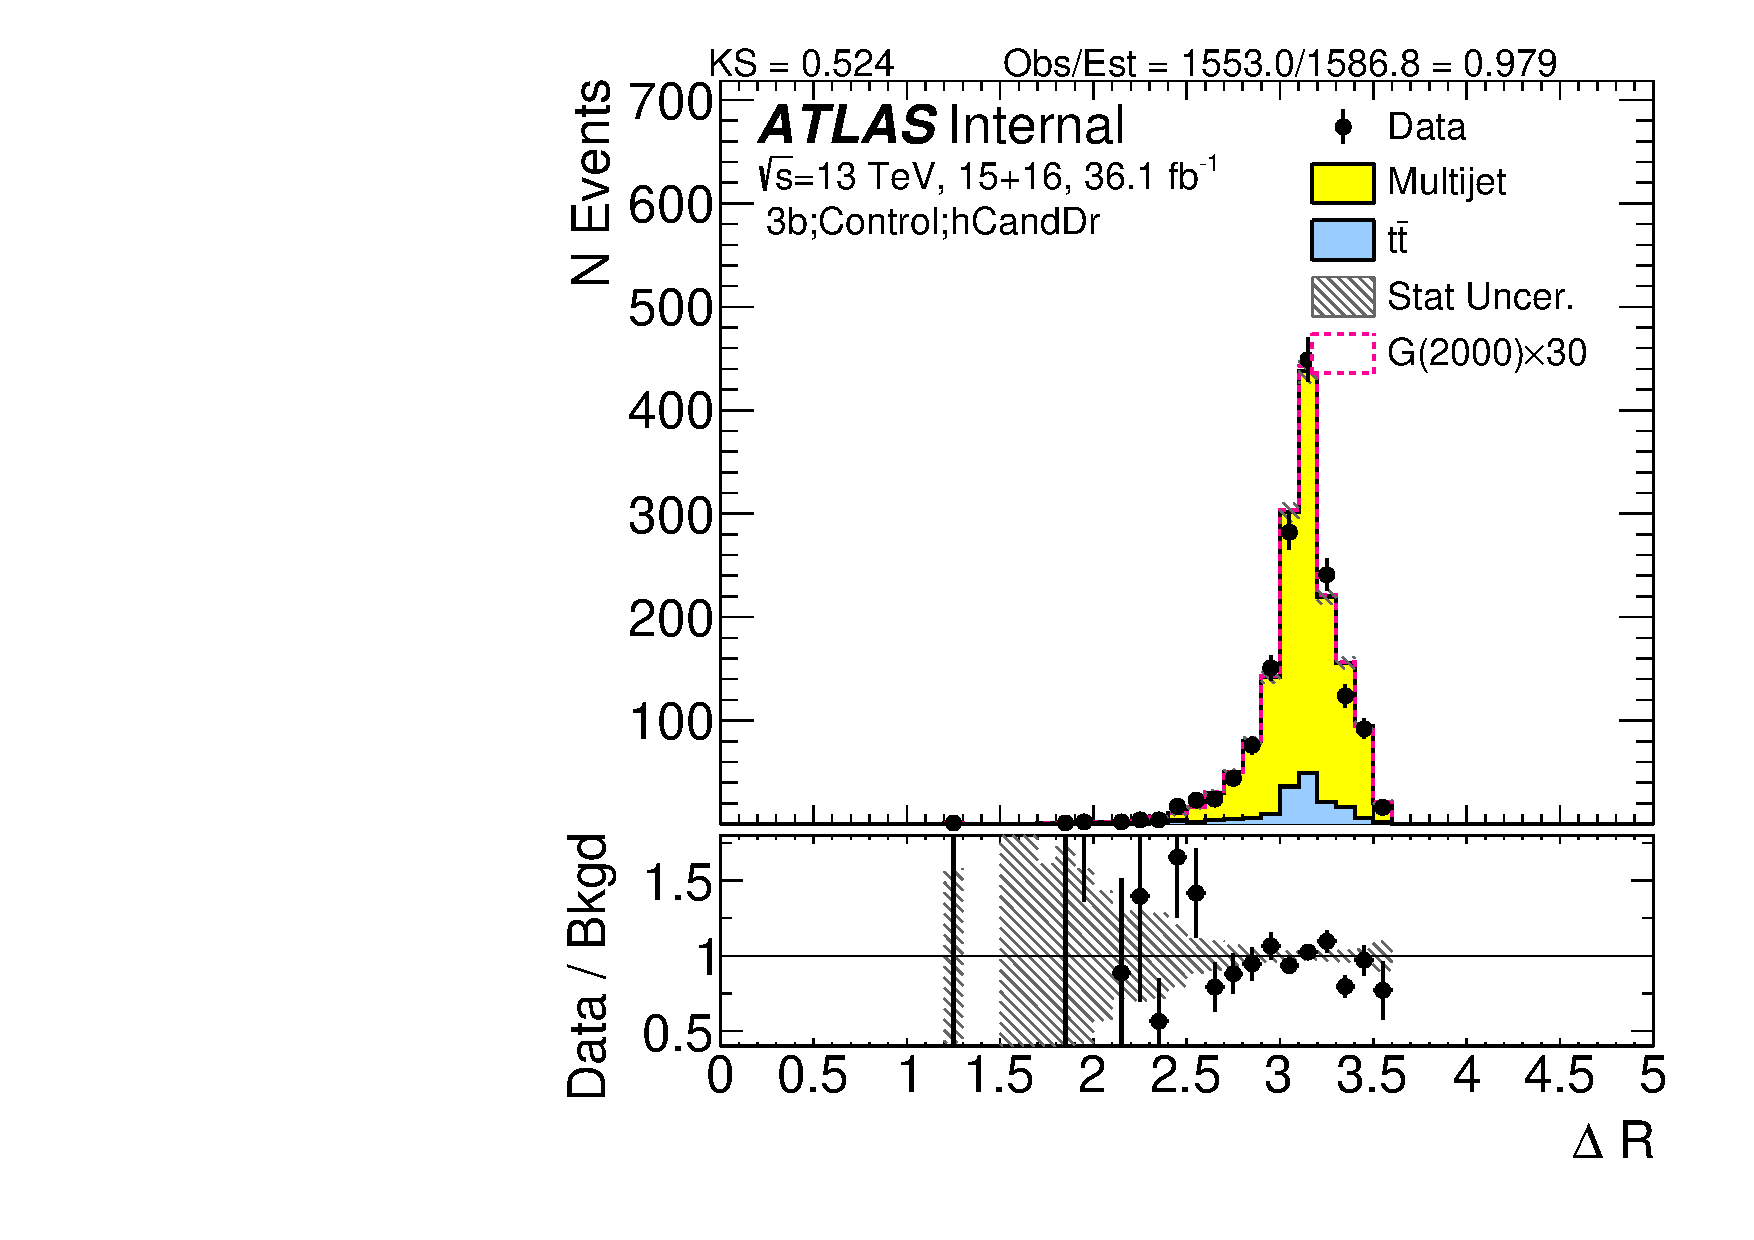
\includegraphics[width=0.32\textwidth,angle=-90]{figures/boosted/Control/b77_ThreeTag_Control_hCandDr.pdf}\\
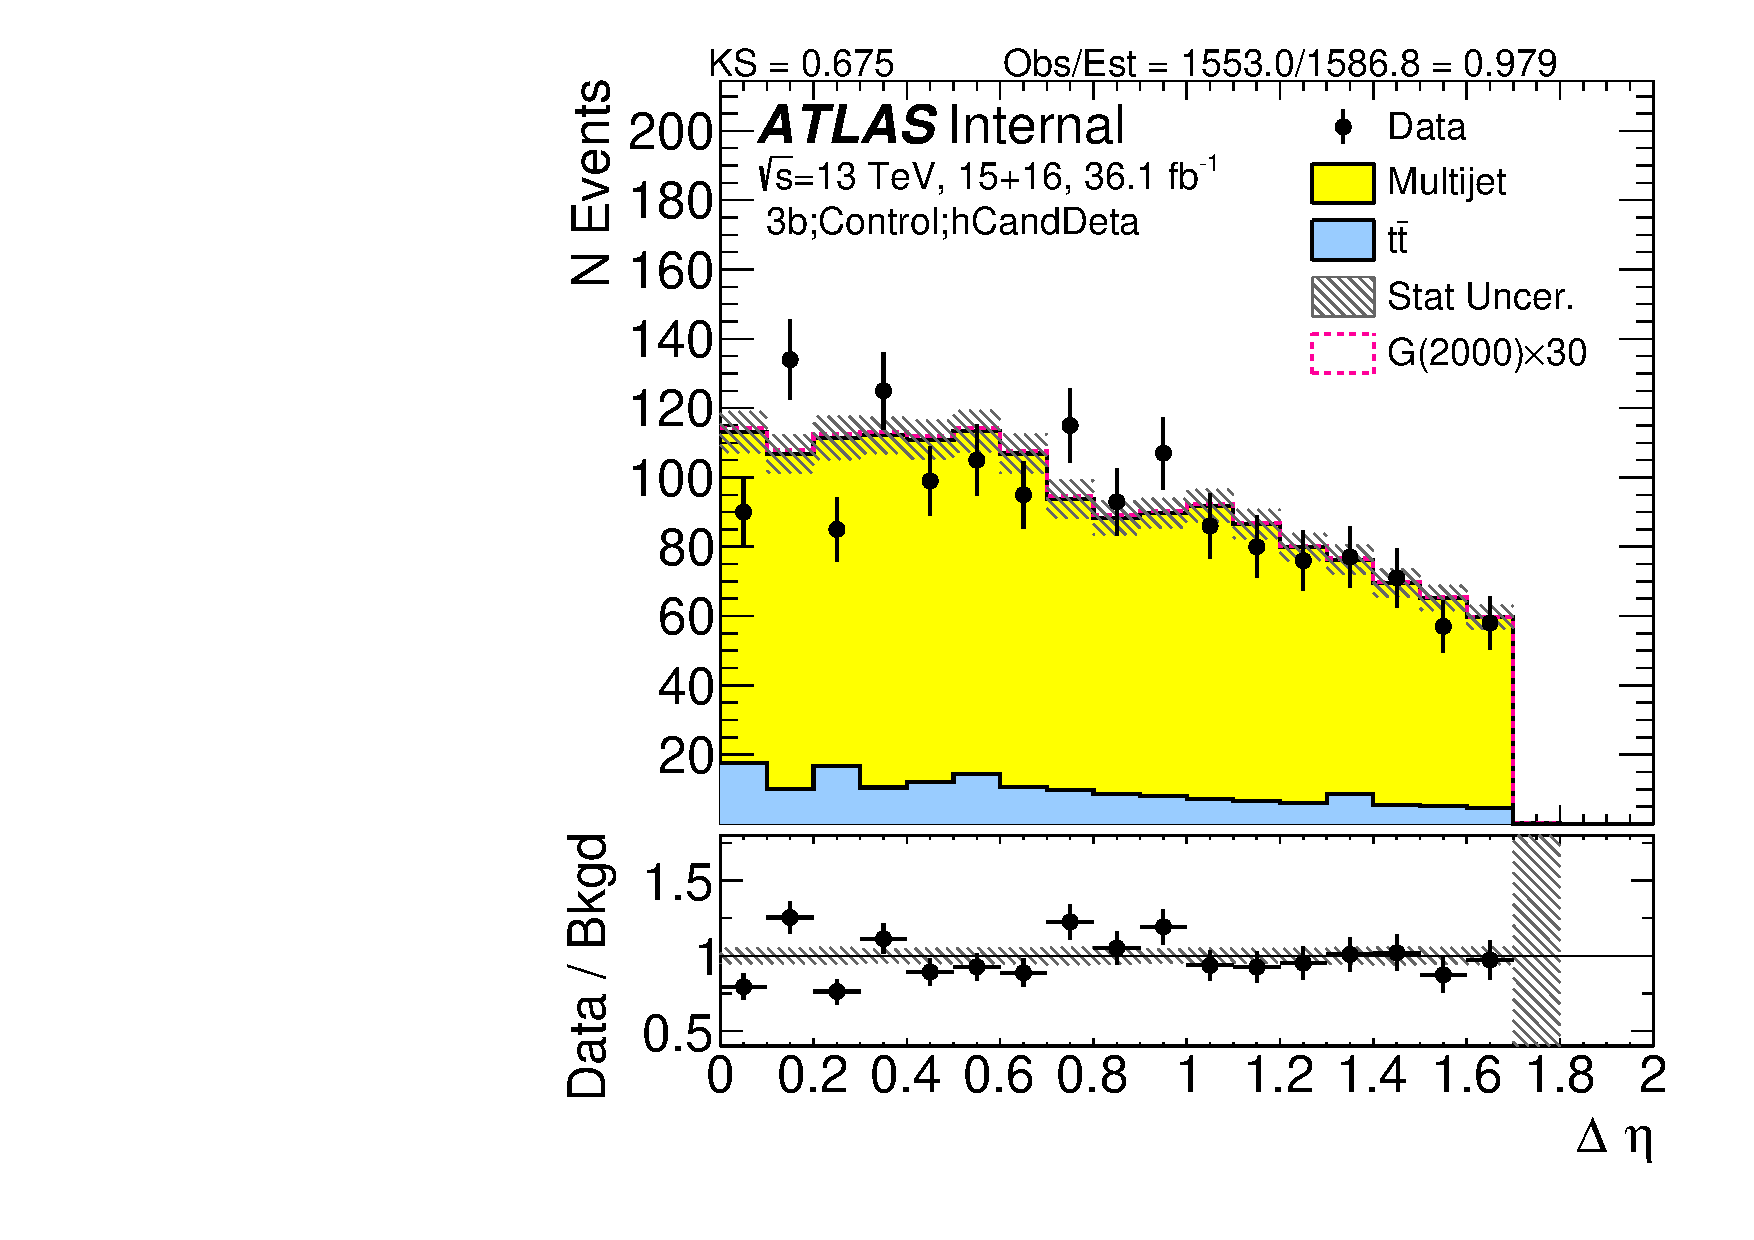
\includegraphics[width=0.32\textwidth,angle=-90]{figures/boosted/Control/b77_ThreeTag_Control_hCandDeta.pdf}
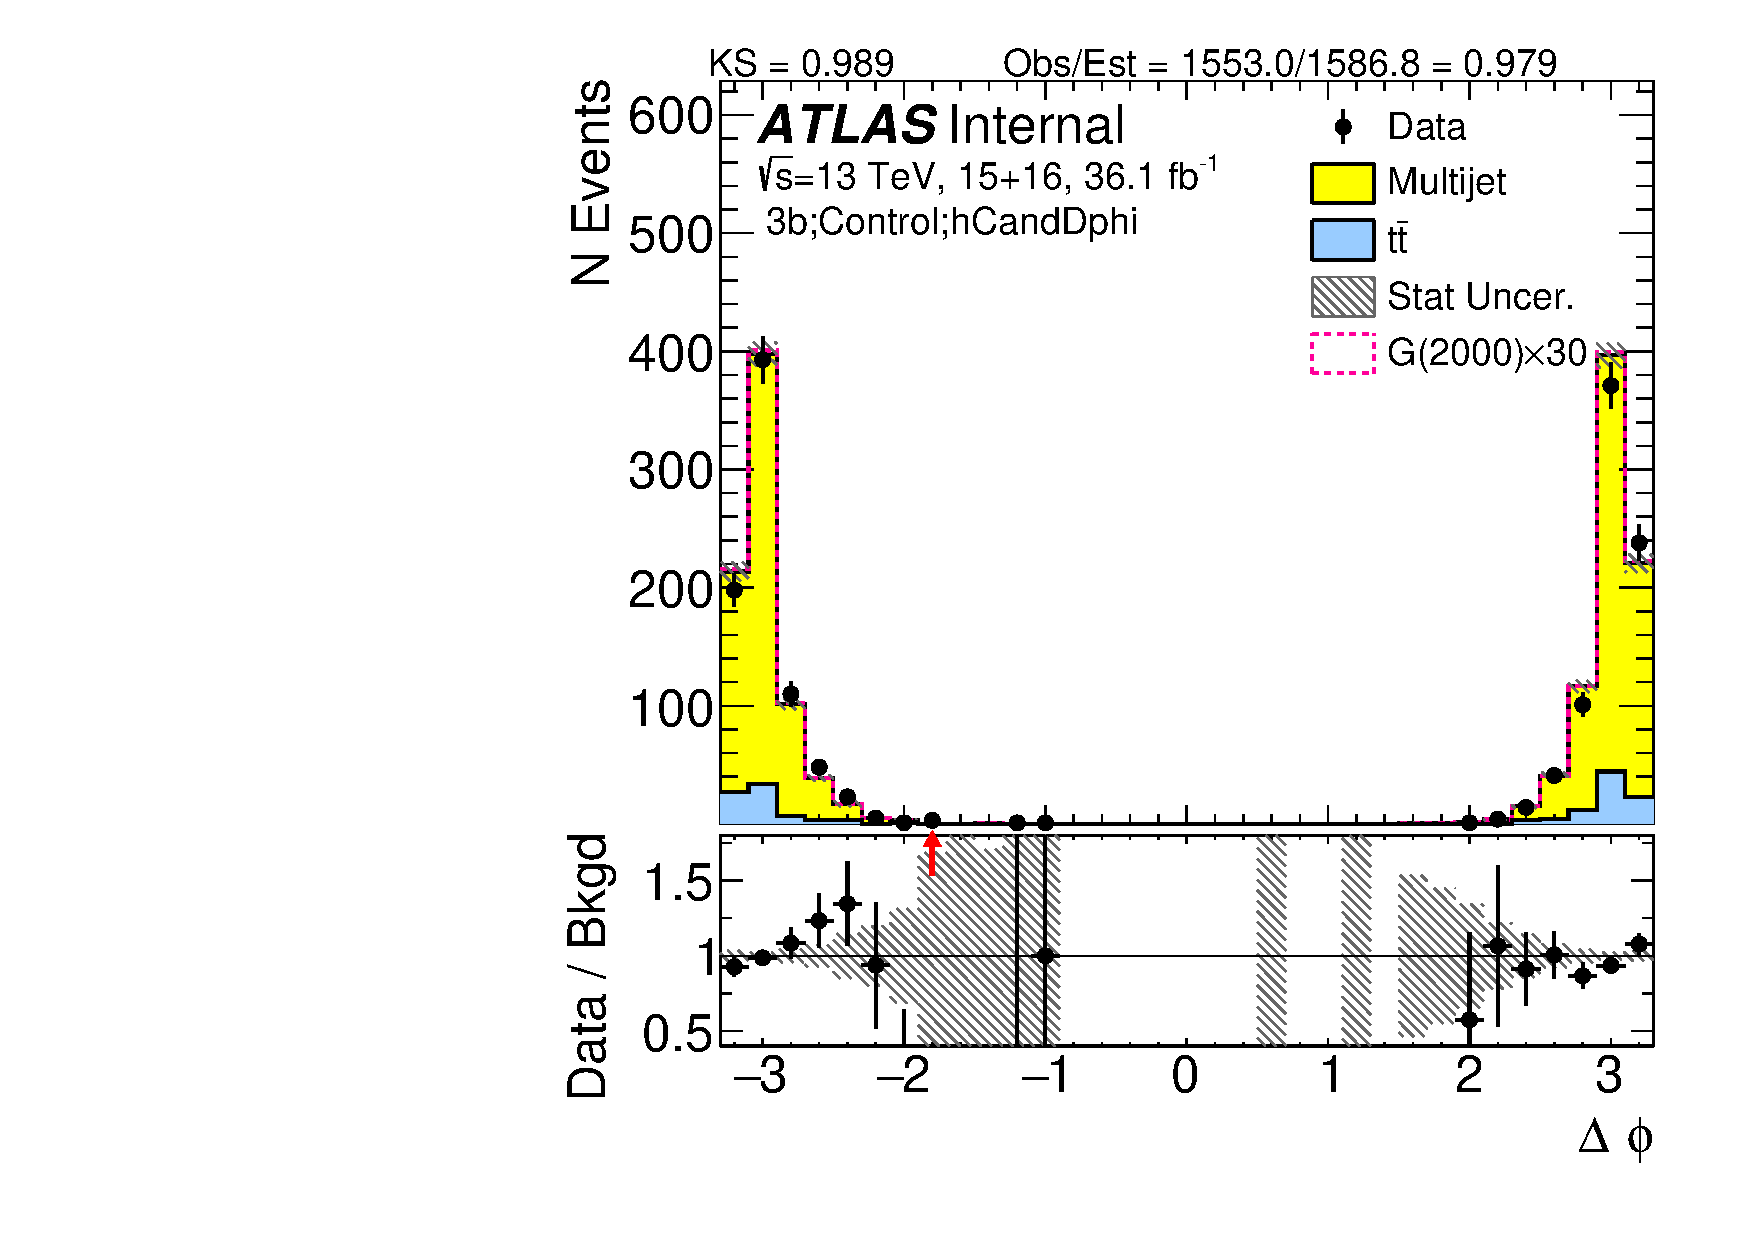
\includegraphics[width=0.32\textwidth,angle=-90]{figures/boosted/Control/b77_ThreeTag_Control_hCandDphi.pdf}
  \caption{Kinematics of the large-\R jet system in data and prediction in the control region after requiring 3 $b$-tags.  }
  \label{fig:boosted-3b-control-ak10-system}
\end{center}
\end{figure*}

\clearpage

\begin{figure*}[htbp!]
\begin{center}
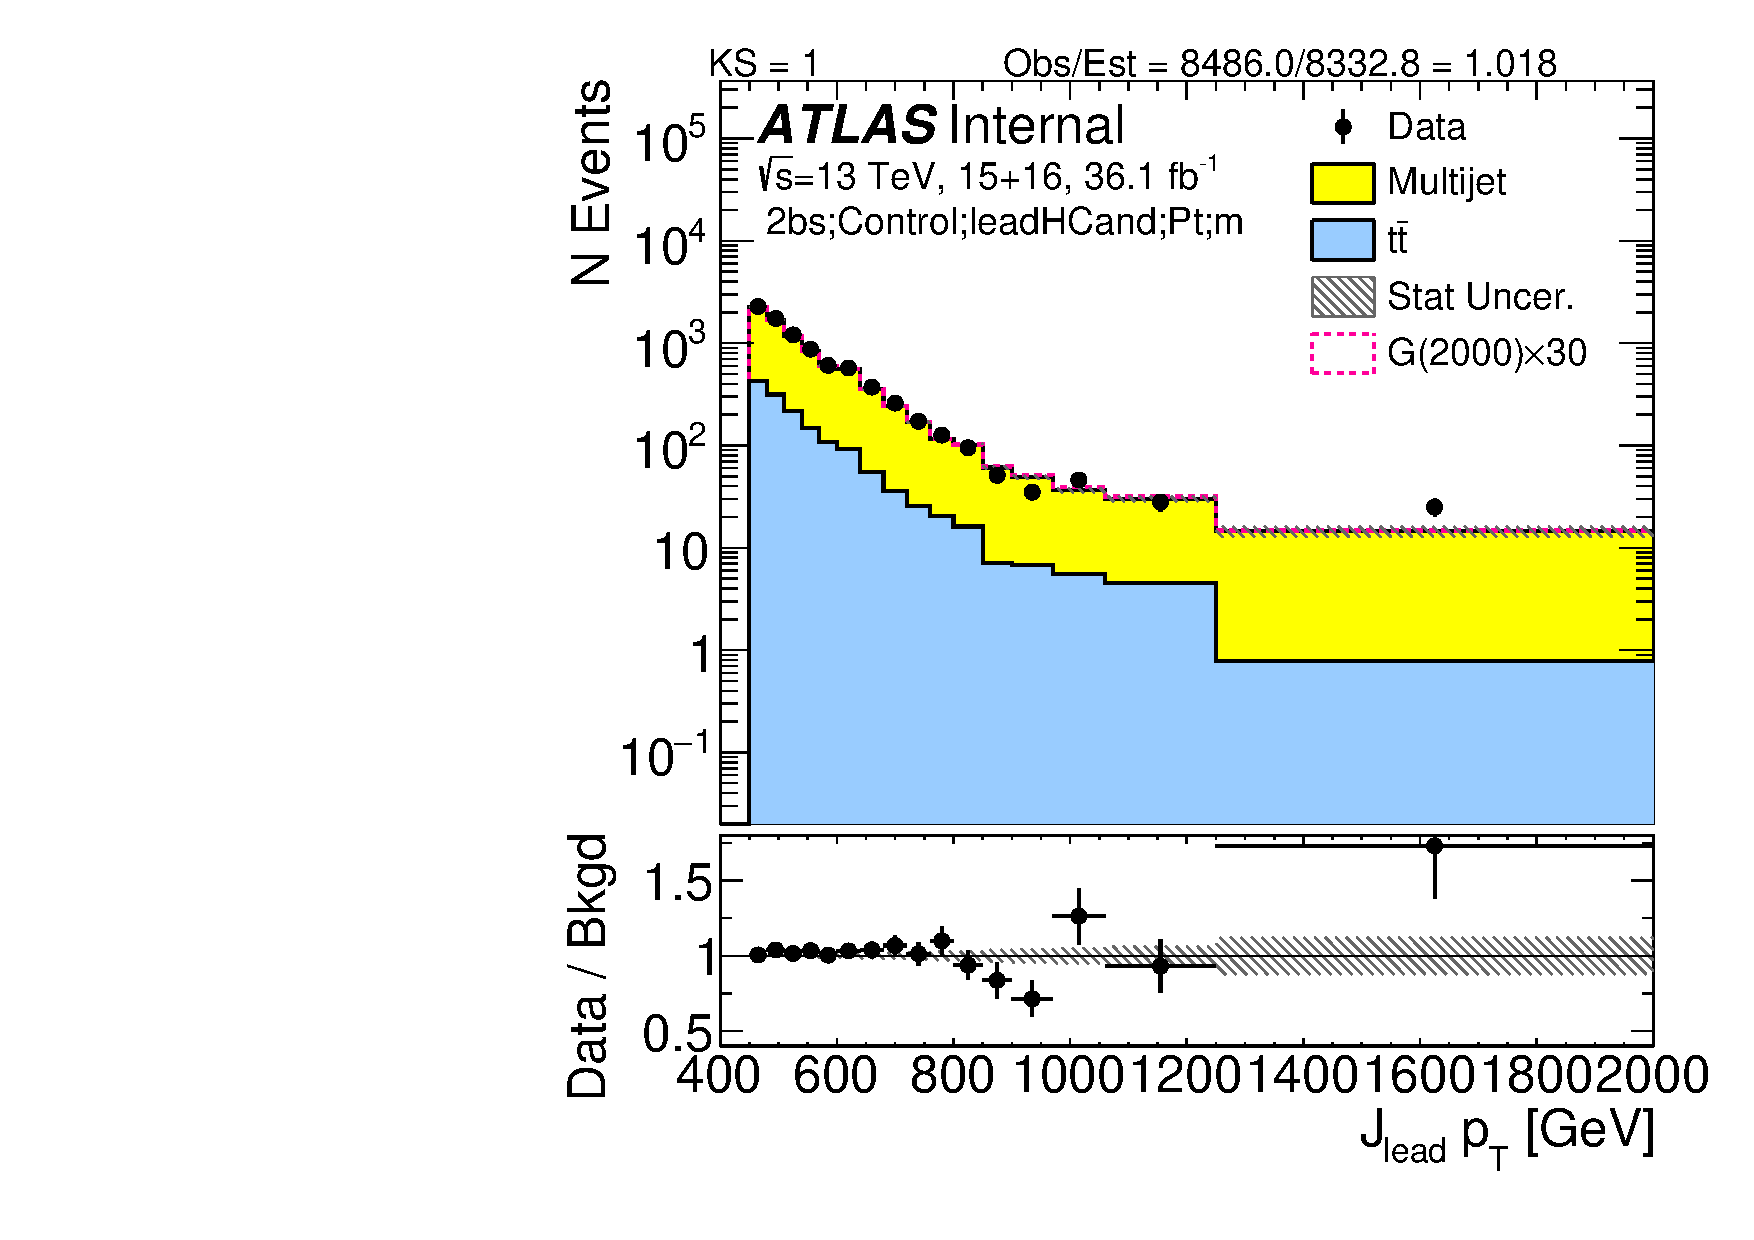
\includegraphics[width=0.32\textwidth,angle=-90]{figures/boosted/Control/b77_TwoTag_split_Control_leadHCand_Pt_m_1.pdf}
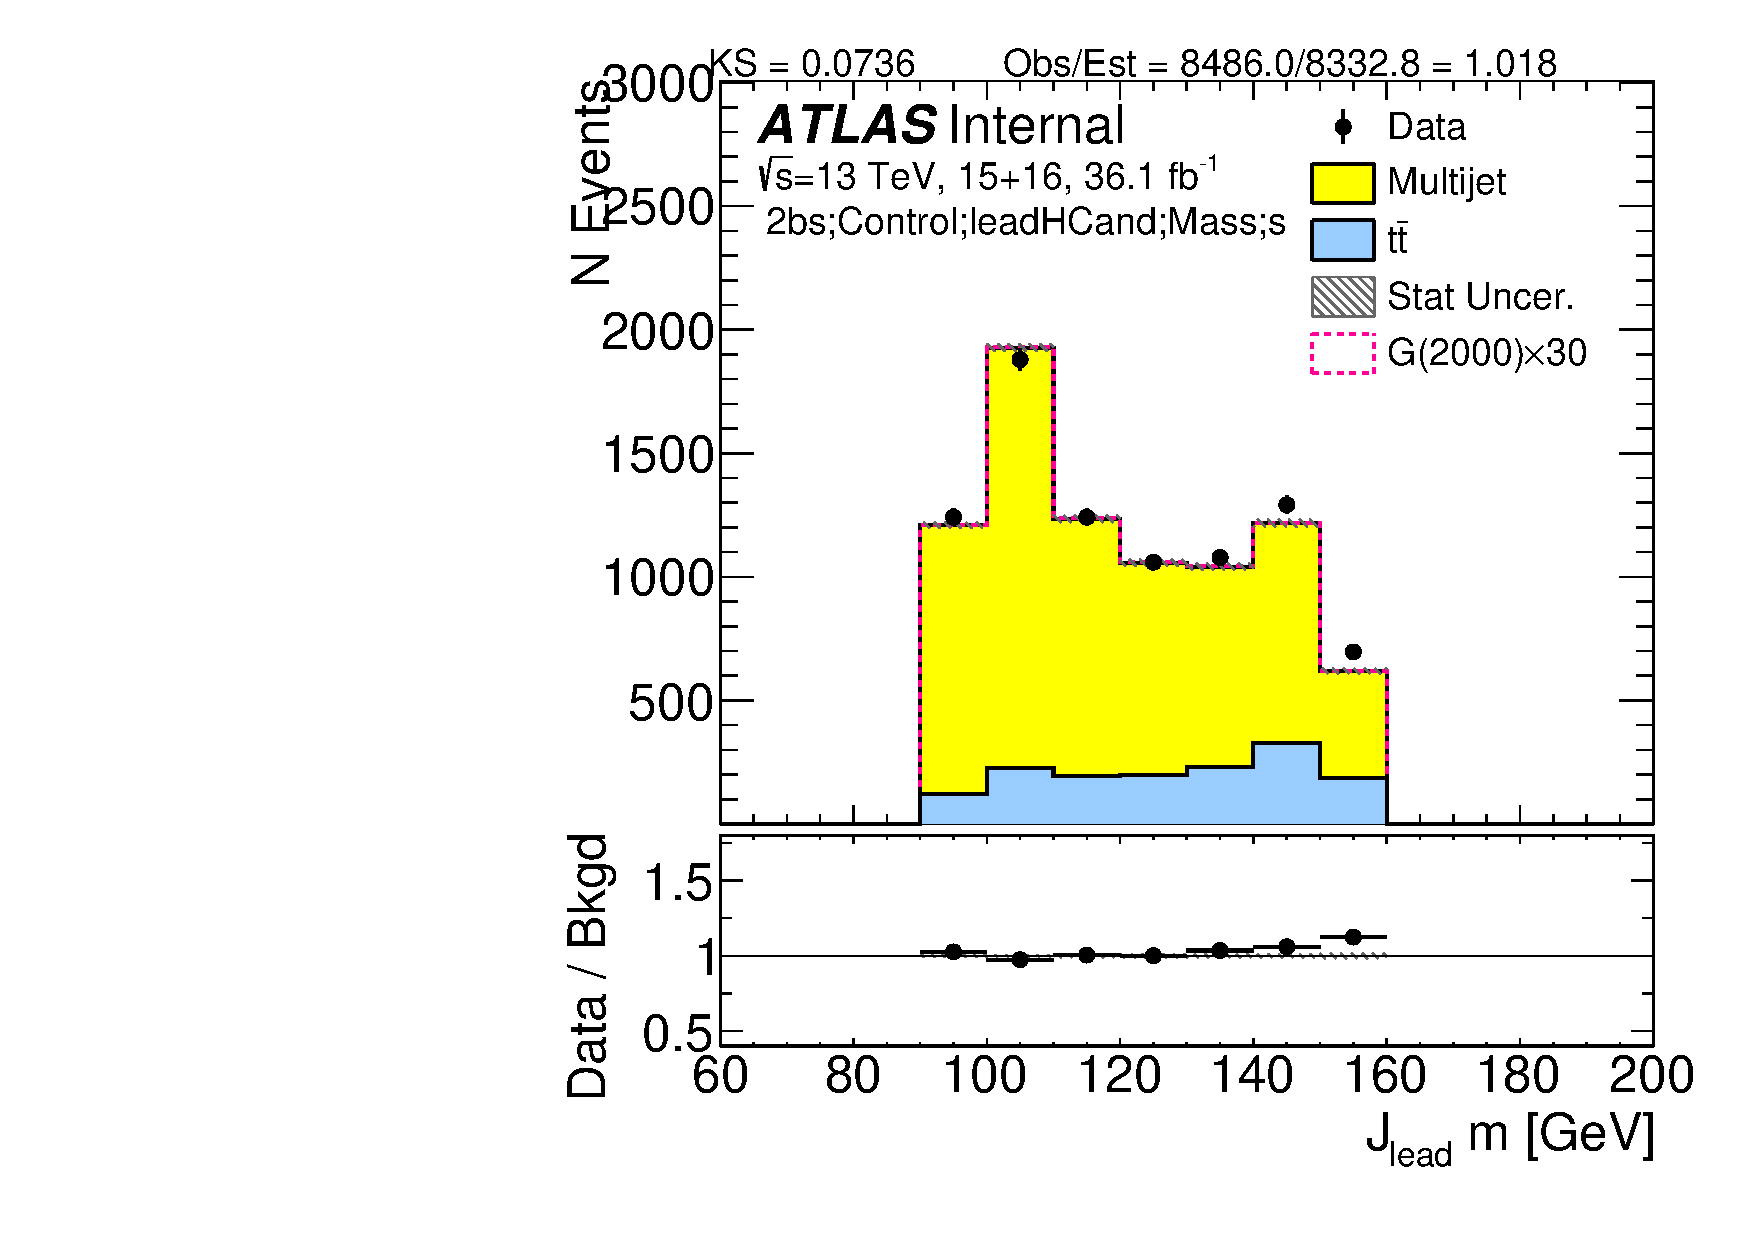
\includegraphics[width=0.32\textwidth,angle=-90]{figures/boosted/Control/b77_TwoTag_split_Control_leadHCand_Mass_s.pdf}\\
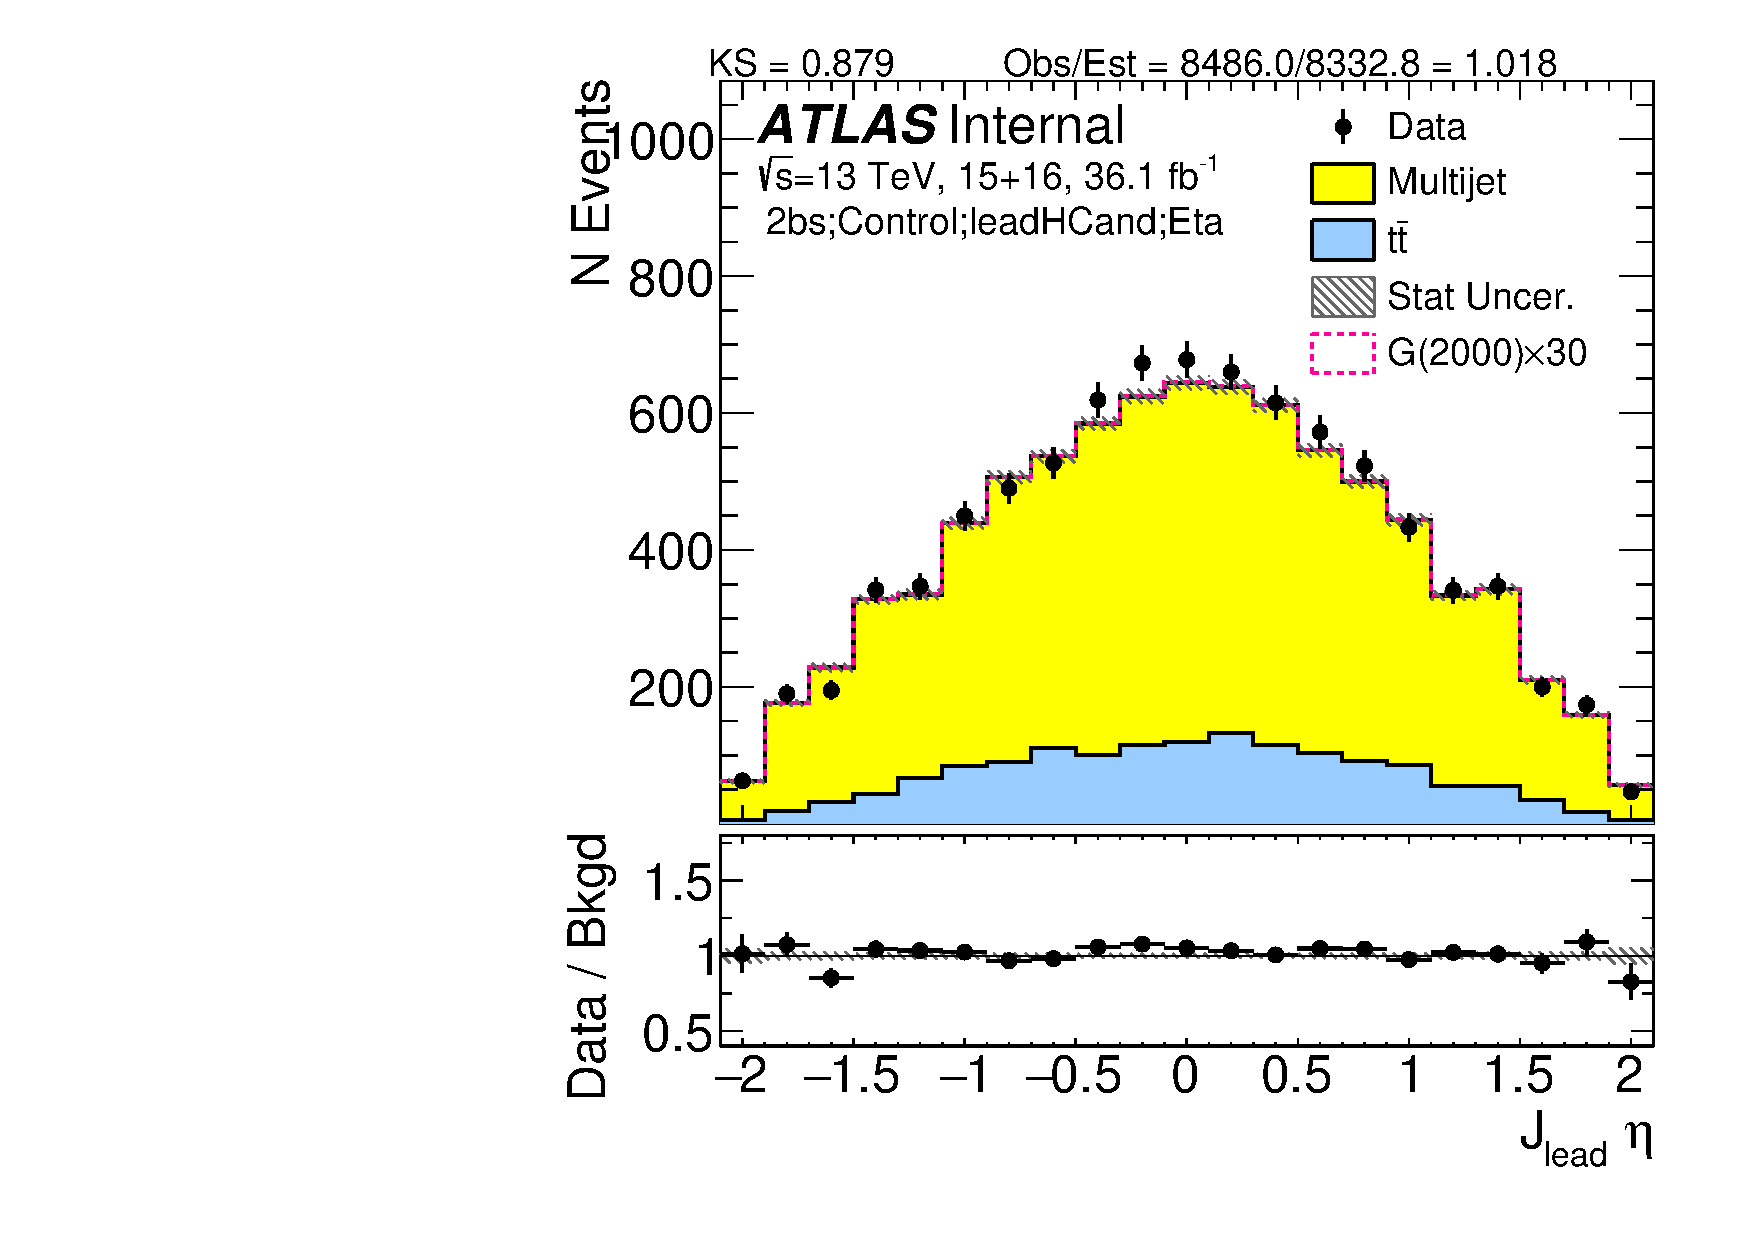
\includegraphics[width=0.32\textwidth,angle=-90]{figures/boosted/Control/b77_TwoTag_split_Control_leadHCand_Eta.pdf}
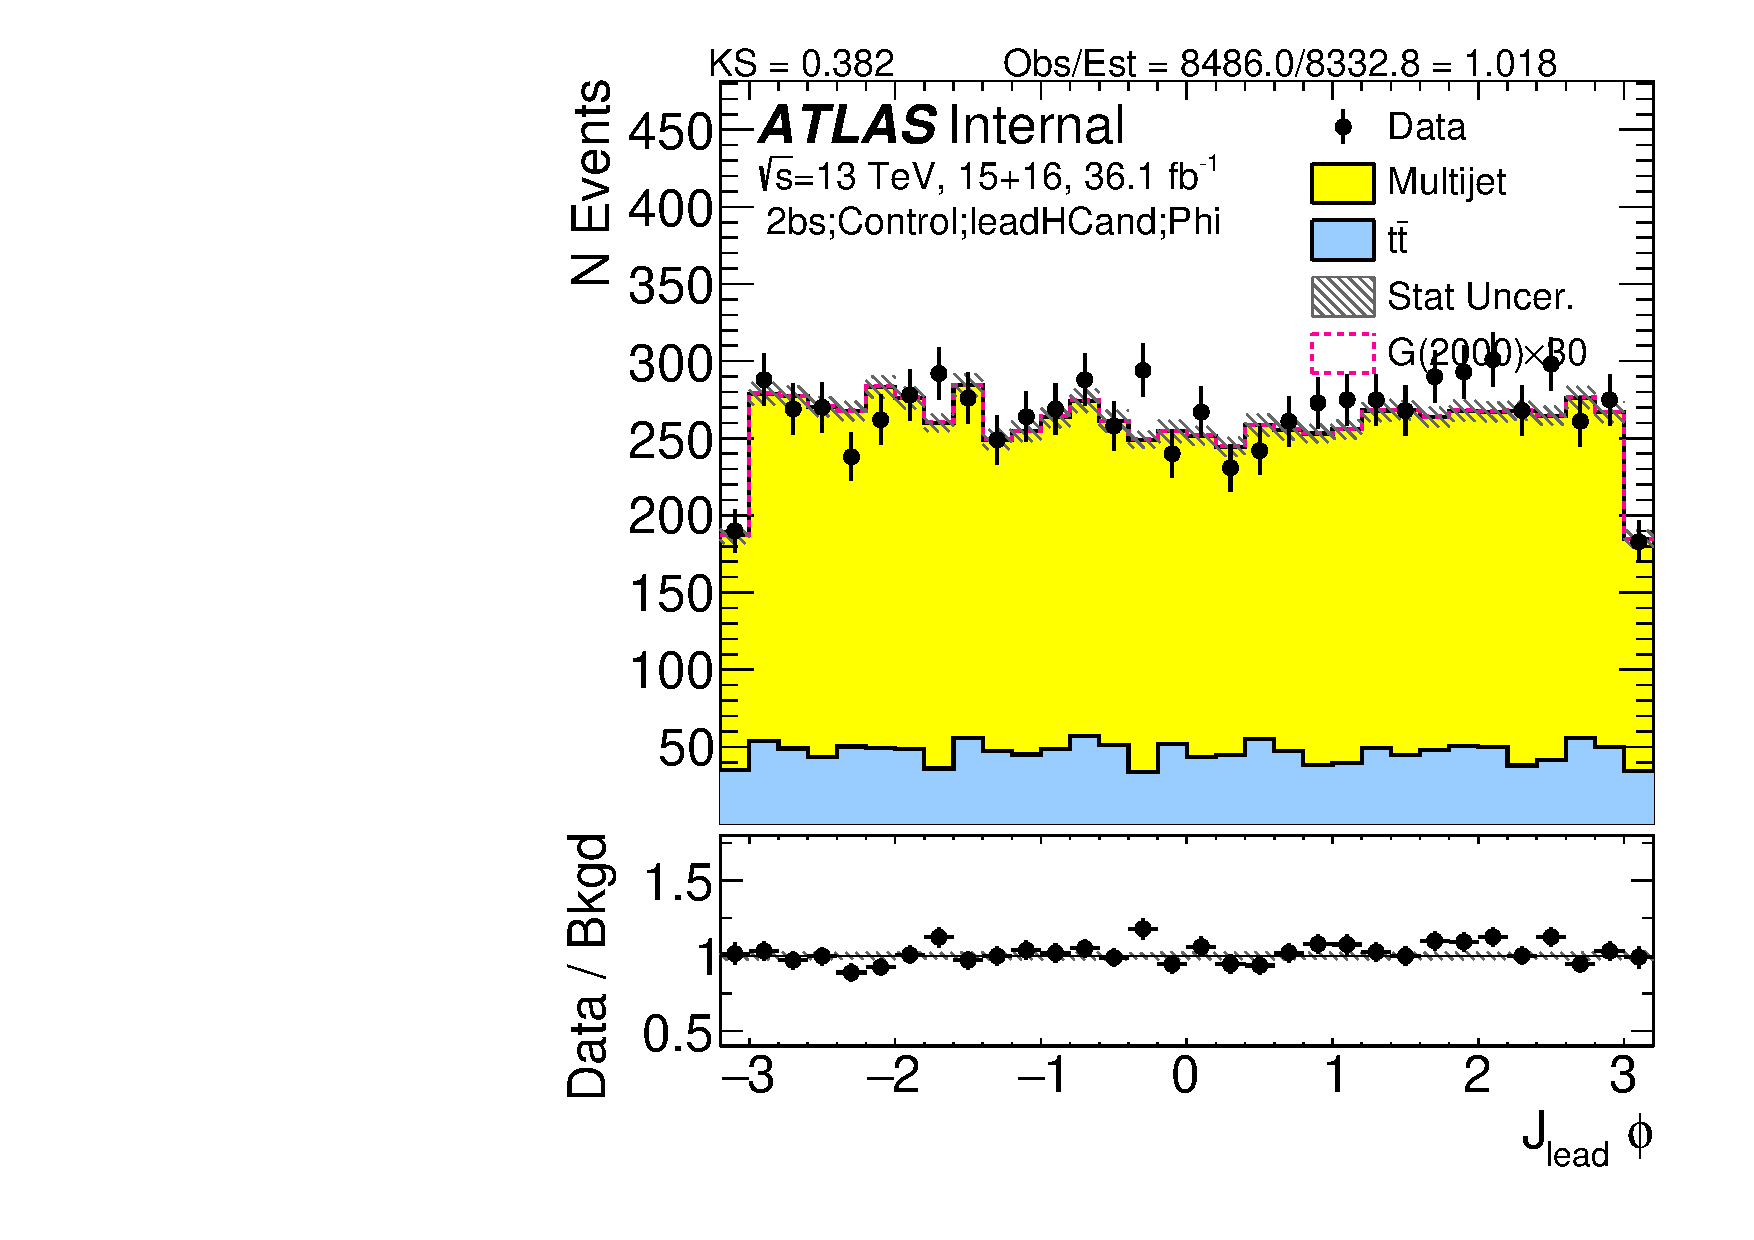
\includegraphics[width=0.32\textwidth,angle=-90]{figures/boosted/Control/b77_TwoTag_split_Control_leadHCand_Phi.pdf}
  \caption{Kinematics of the lead large-\R jet in data and prediction in the control region after requiring 2 $b$-tags split. }
  \label{fig:boosted-2bs-control-ak10-lead}
\end{center}
\end{figure*}

\begin{figure*}[htbp!]
\begin{center}
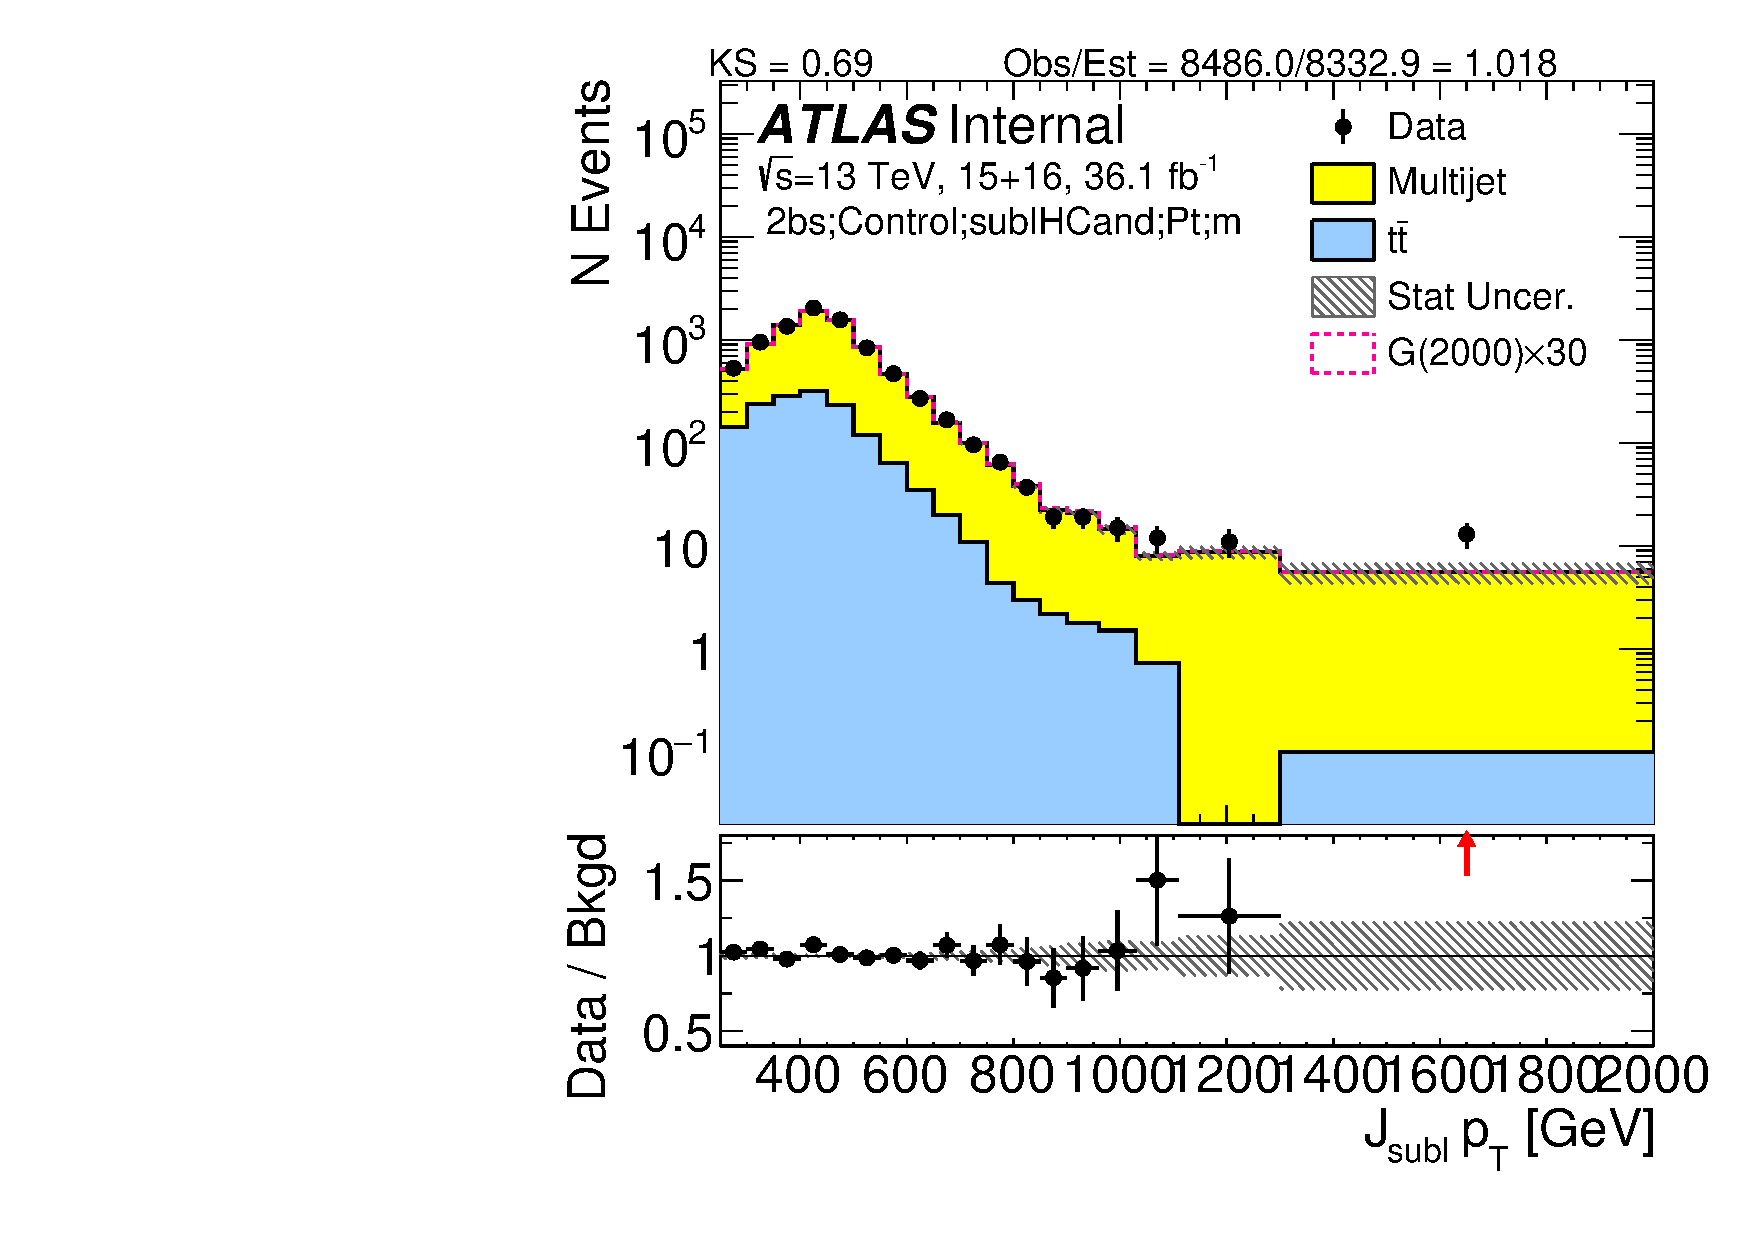
\includegraphics[width=0.32\textwidth,angle=-90]{figures/boosted/Control/b77_TwoTag_split_Control_sublHCand_Pt_m_1.pdf}
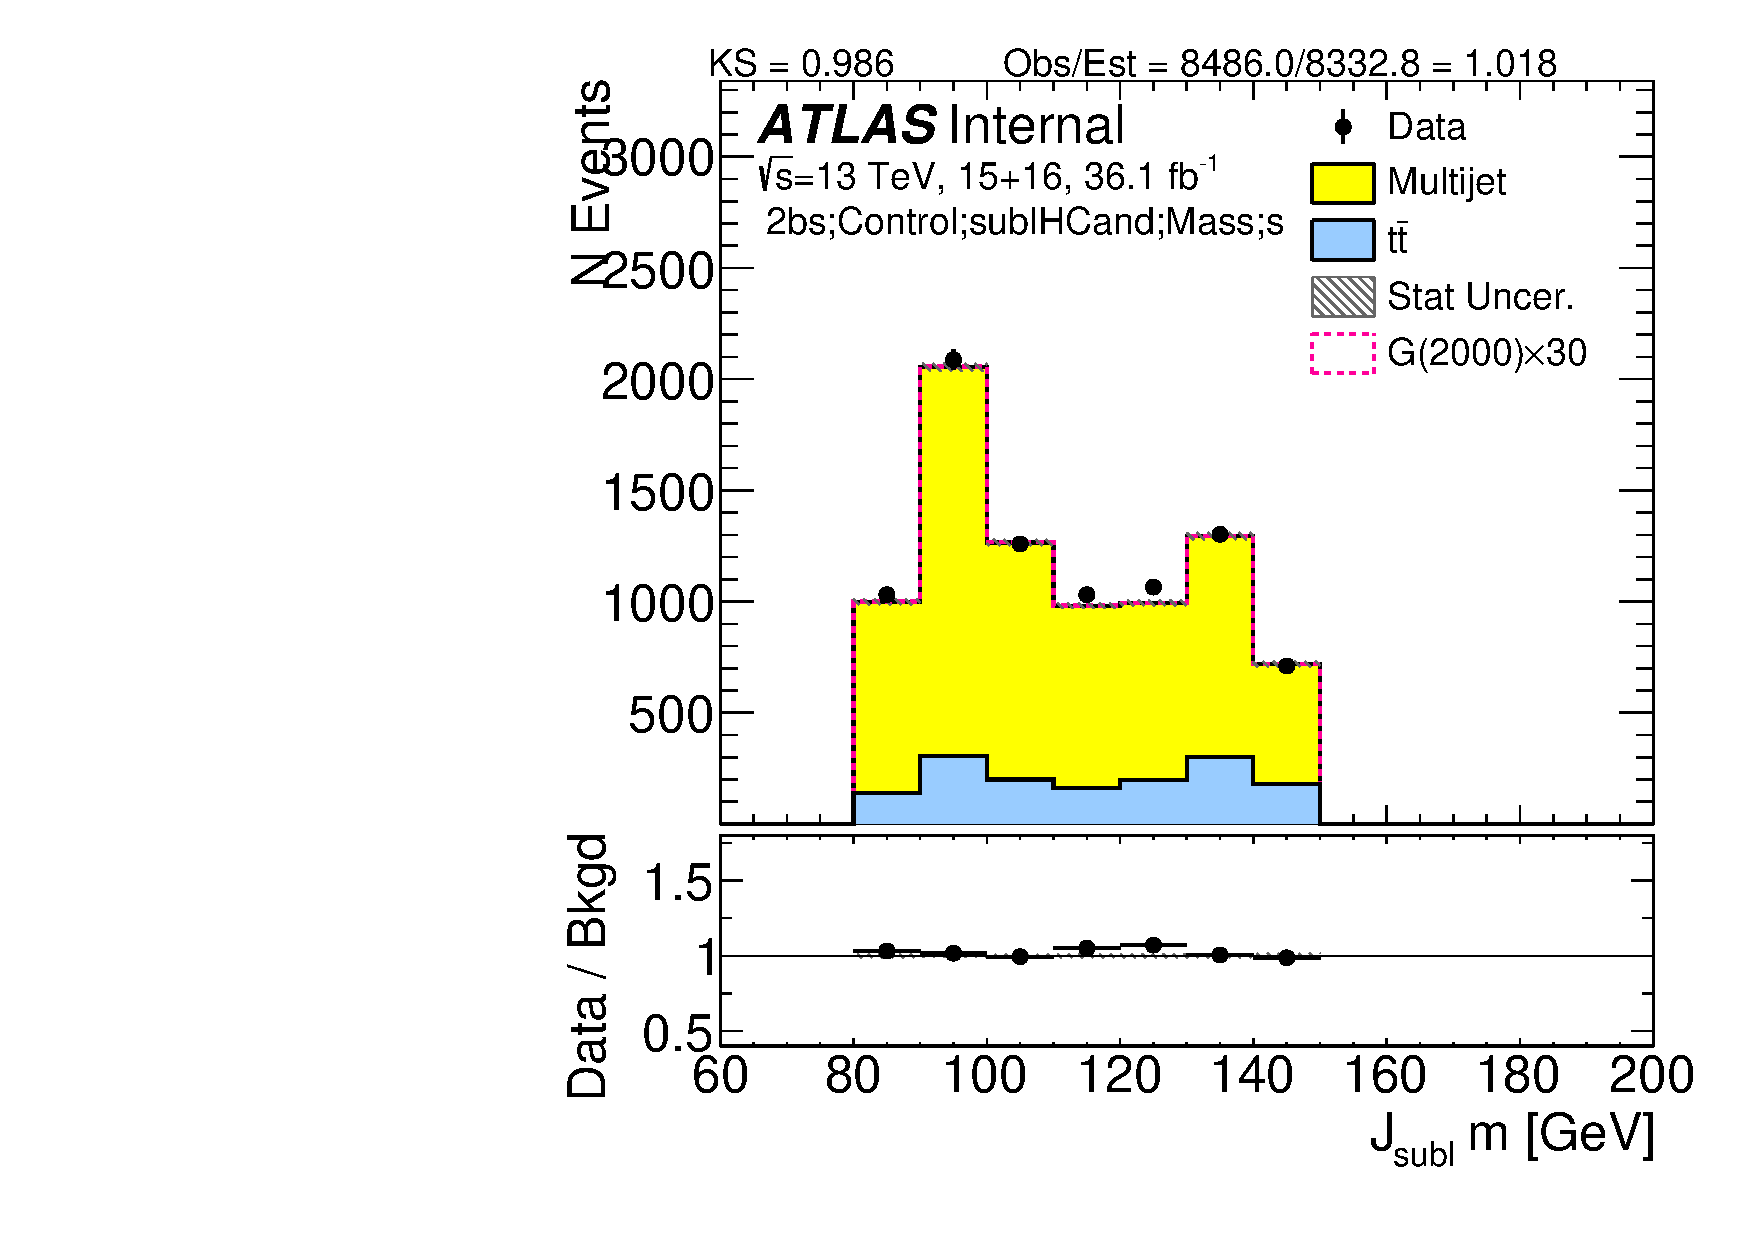
\includegraphics[width=0.32\textwidth,angle=-90]{figures/boosted/Control/b77_TwoTag_split_Control_sublHCand_Mass_s.pdf}\\
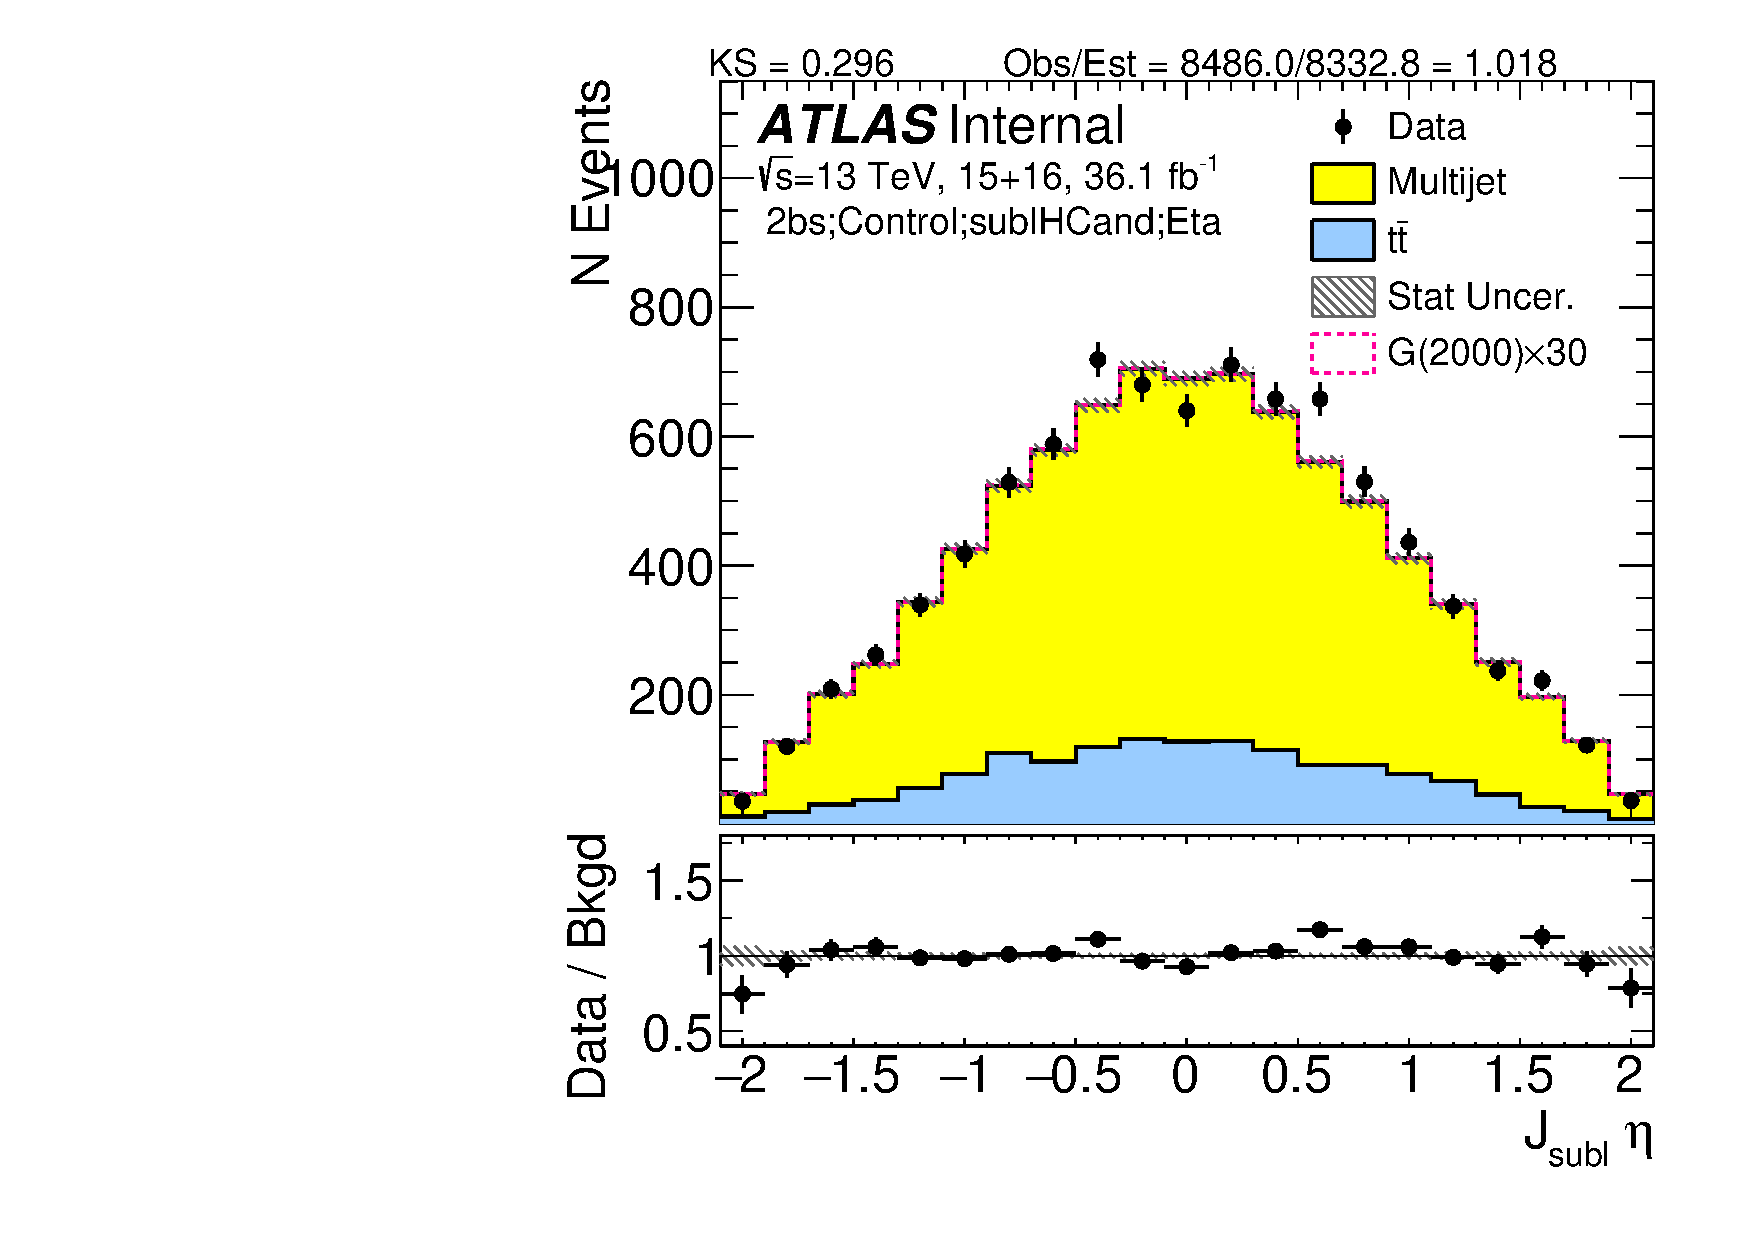
\includegraphics[width=0.32\textwidth,angle=-90]{figures/boosted/Control/b77_TwoTag_split_Control_sublHCand_Eta.pdf}
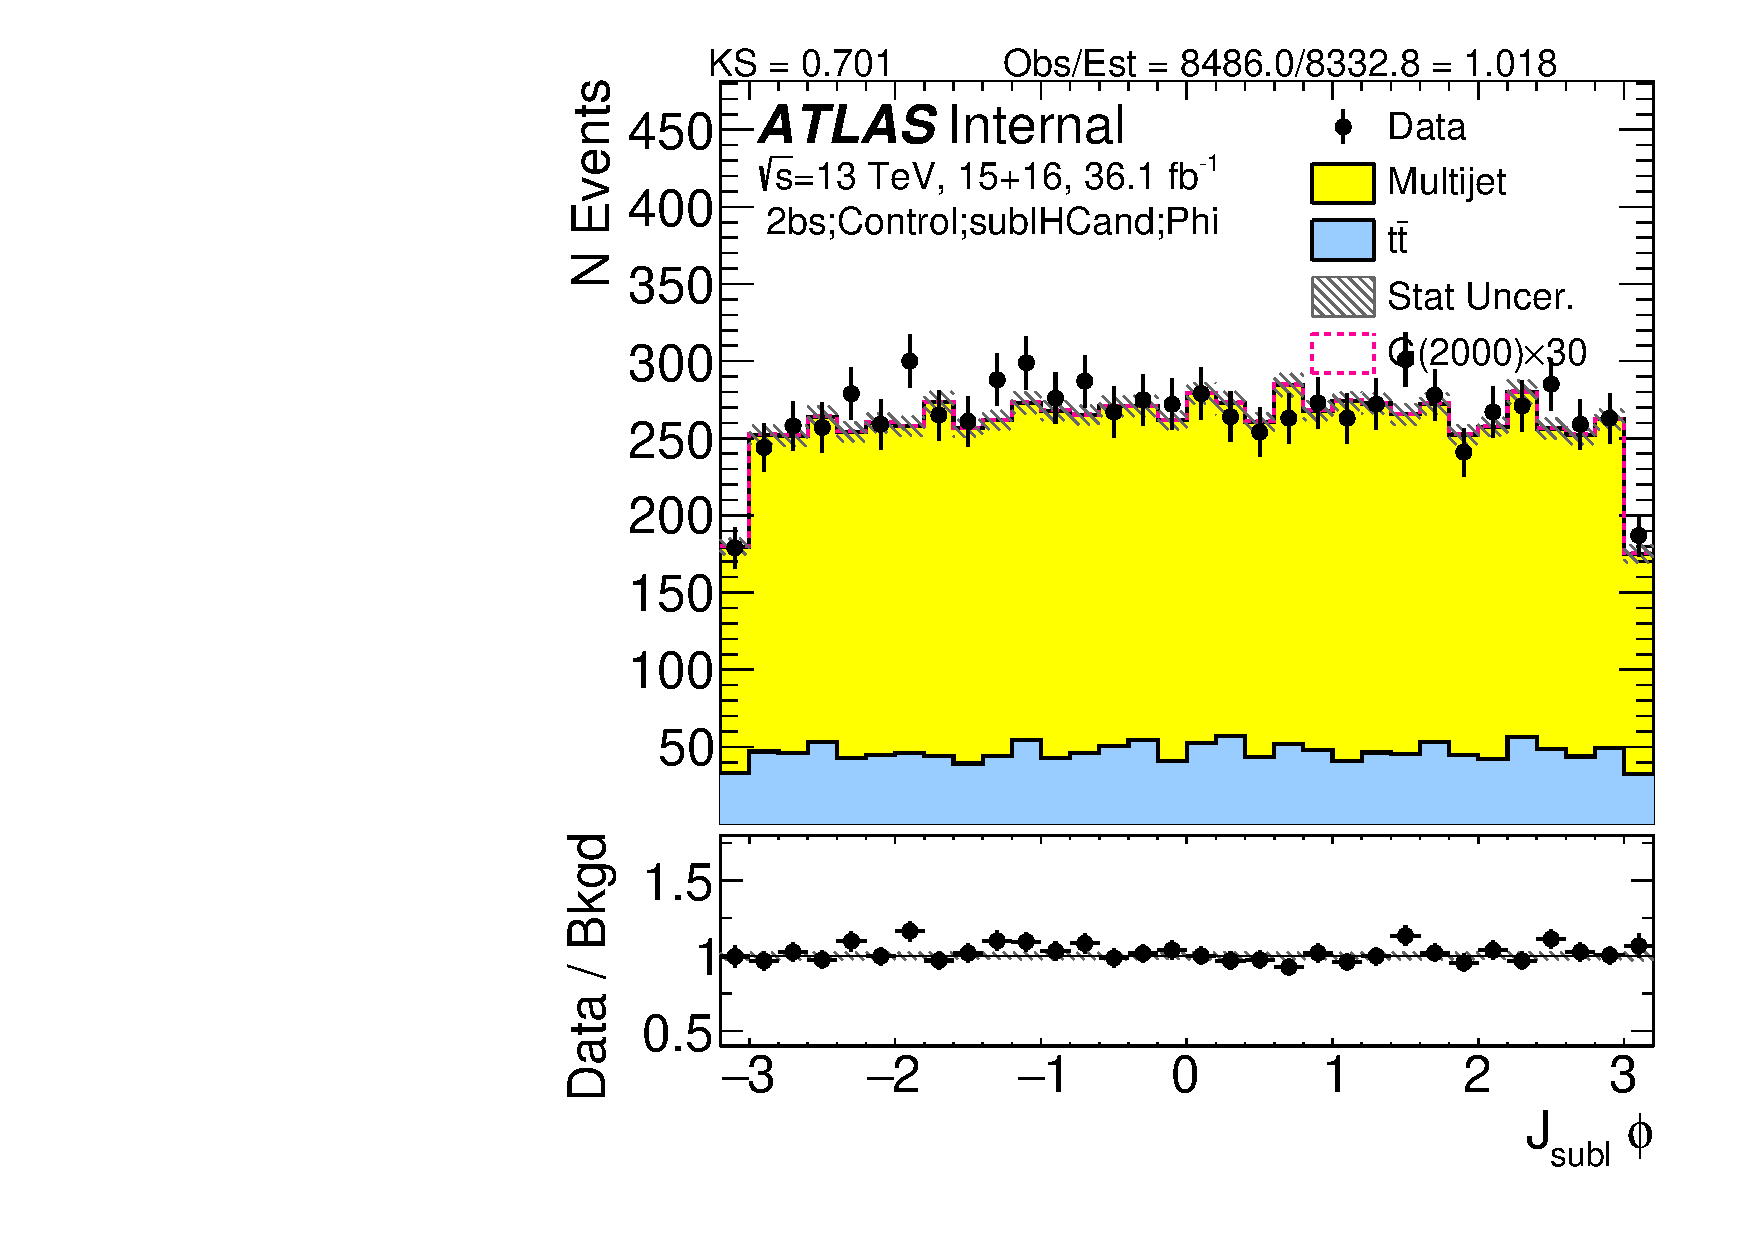
\includegraphics[width=0.32\textwidth,angle=-90]{figures/boosted/Control/b77_TwoTag_split_Control_sublHCand_Phi.pdf}
  \caption{Kinematics of the sub-lead large-\R jet in data and prediction in the control region after requiring 2 $b$-tags split. }
  \label{fig:boosted-2bs-control-ak10-subl}
\end{center}
\end{figure*}

\begin{figure*}[htbp!]
\begin{center}
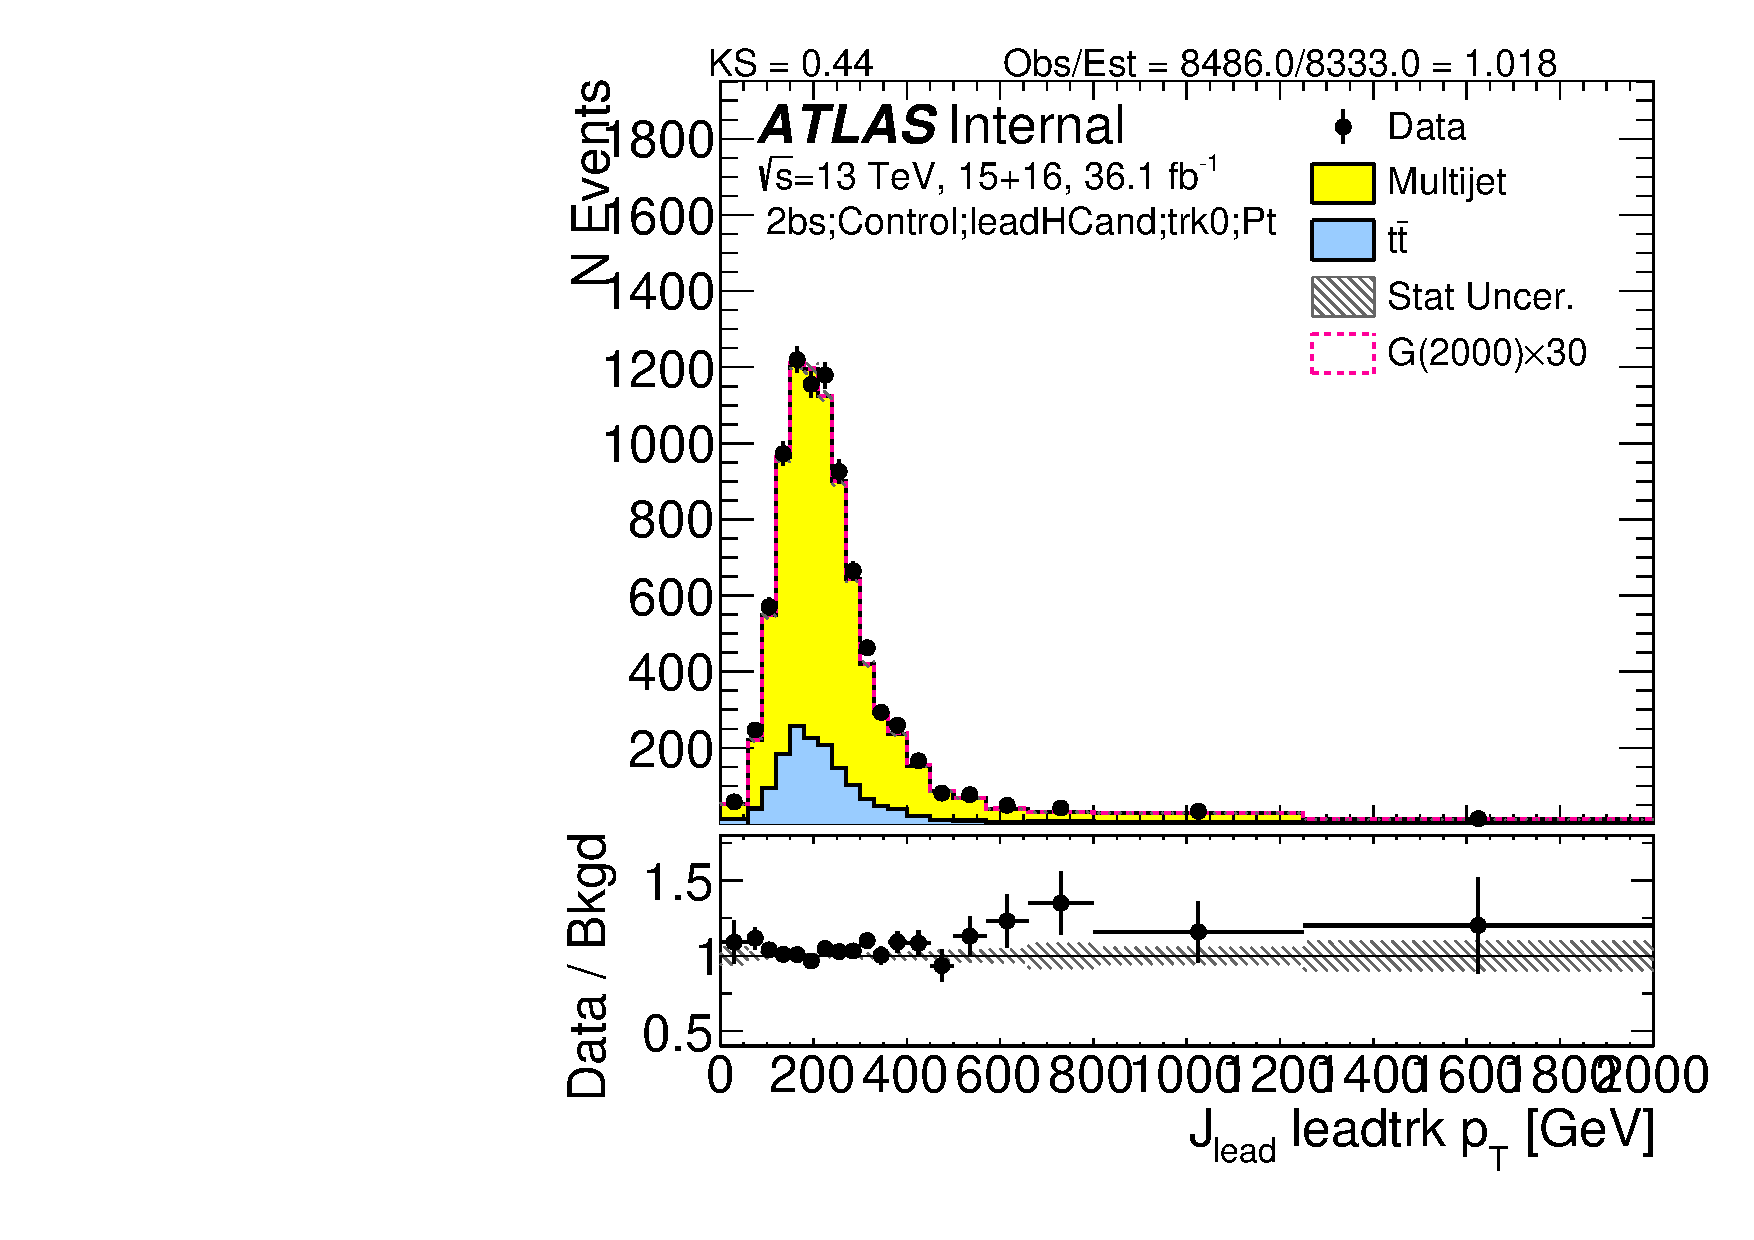
\includegraphics[width=0.32\textwidth,angle=-90]{figures/boosted/Control/b77_TwoTag_split_Control_leadHCand_trk0_Pt.pdf}
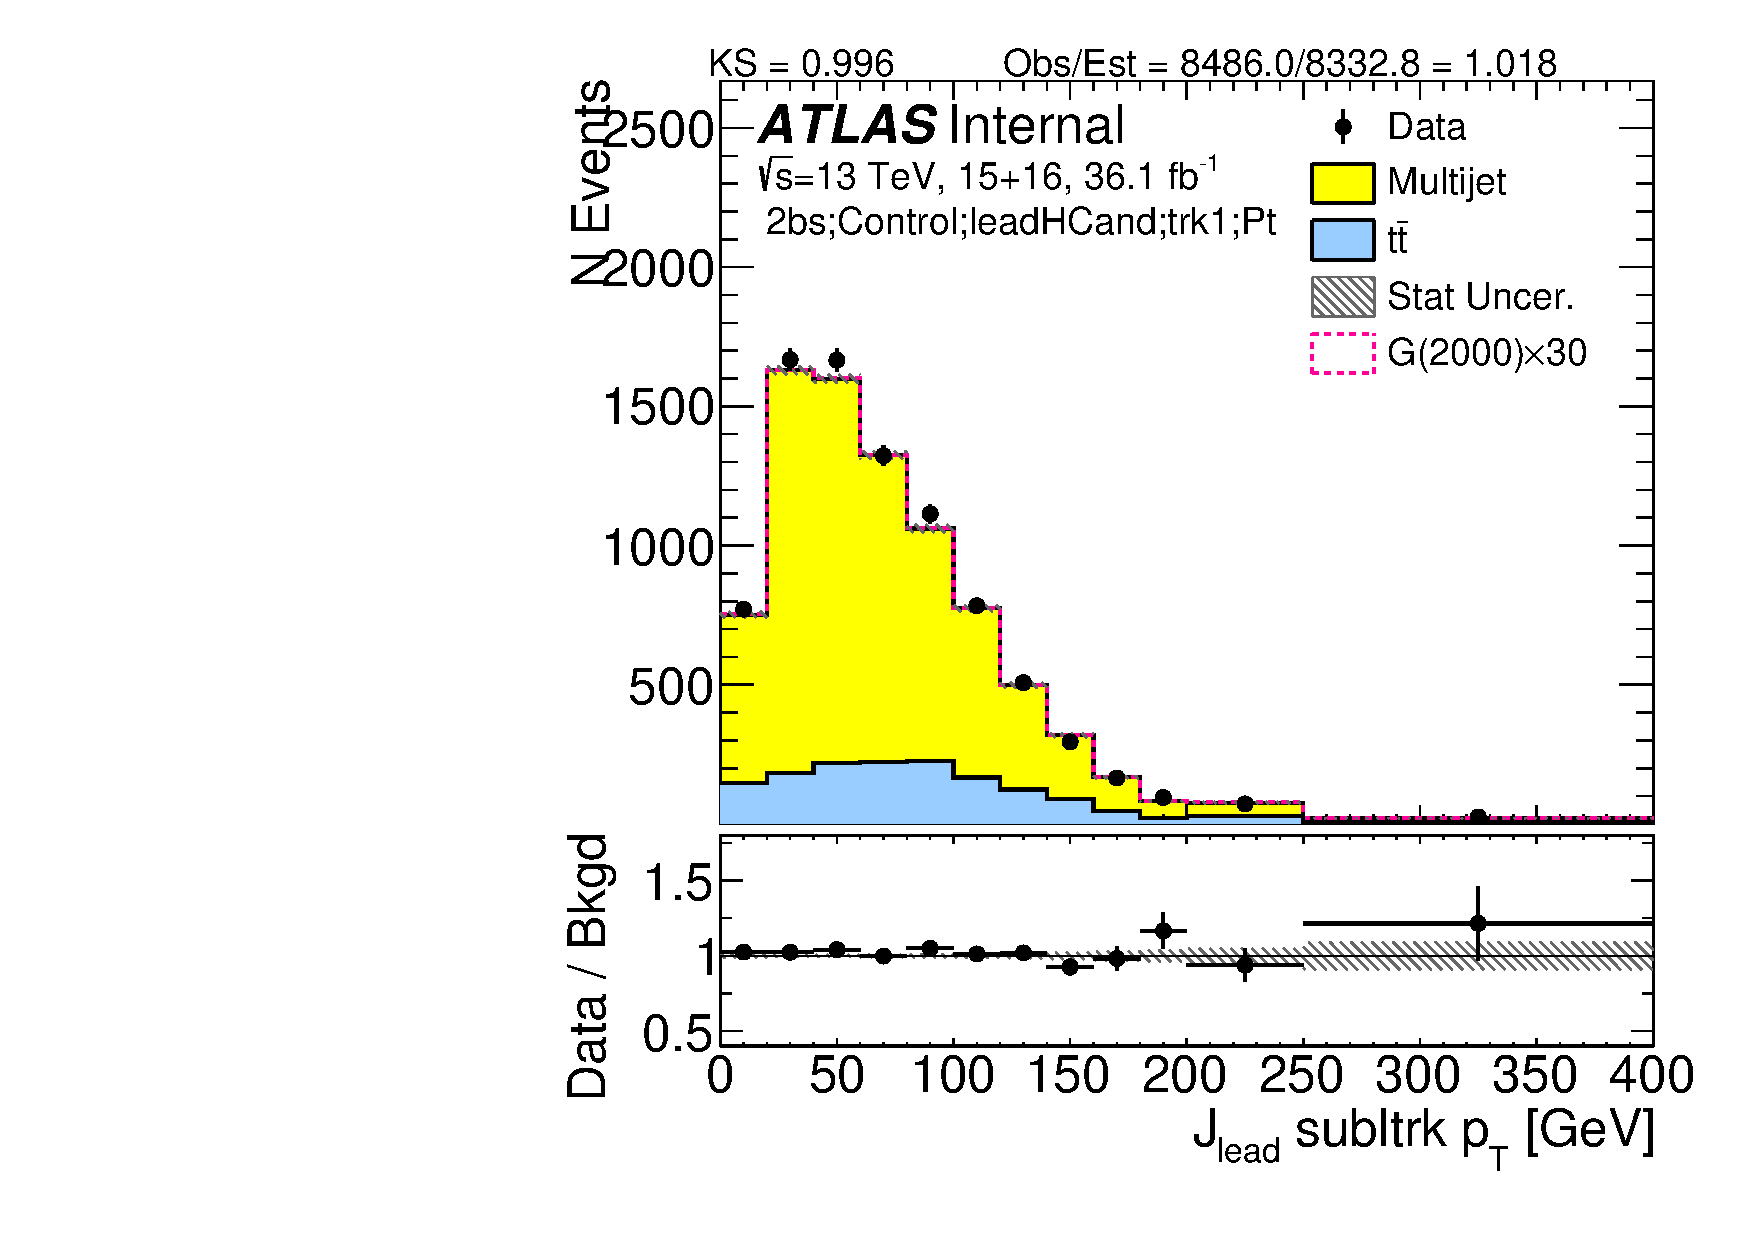
\includegraphics[width=0.32\textwidth,angle=-90]{figures/boosted/Control/b77_TwoTag_split_Control_leadHCand_trk1_Pt.pdf}\\
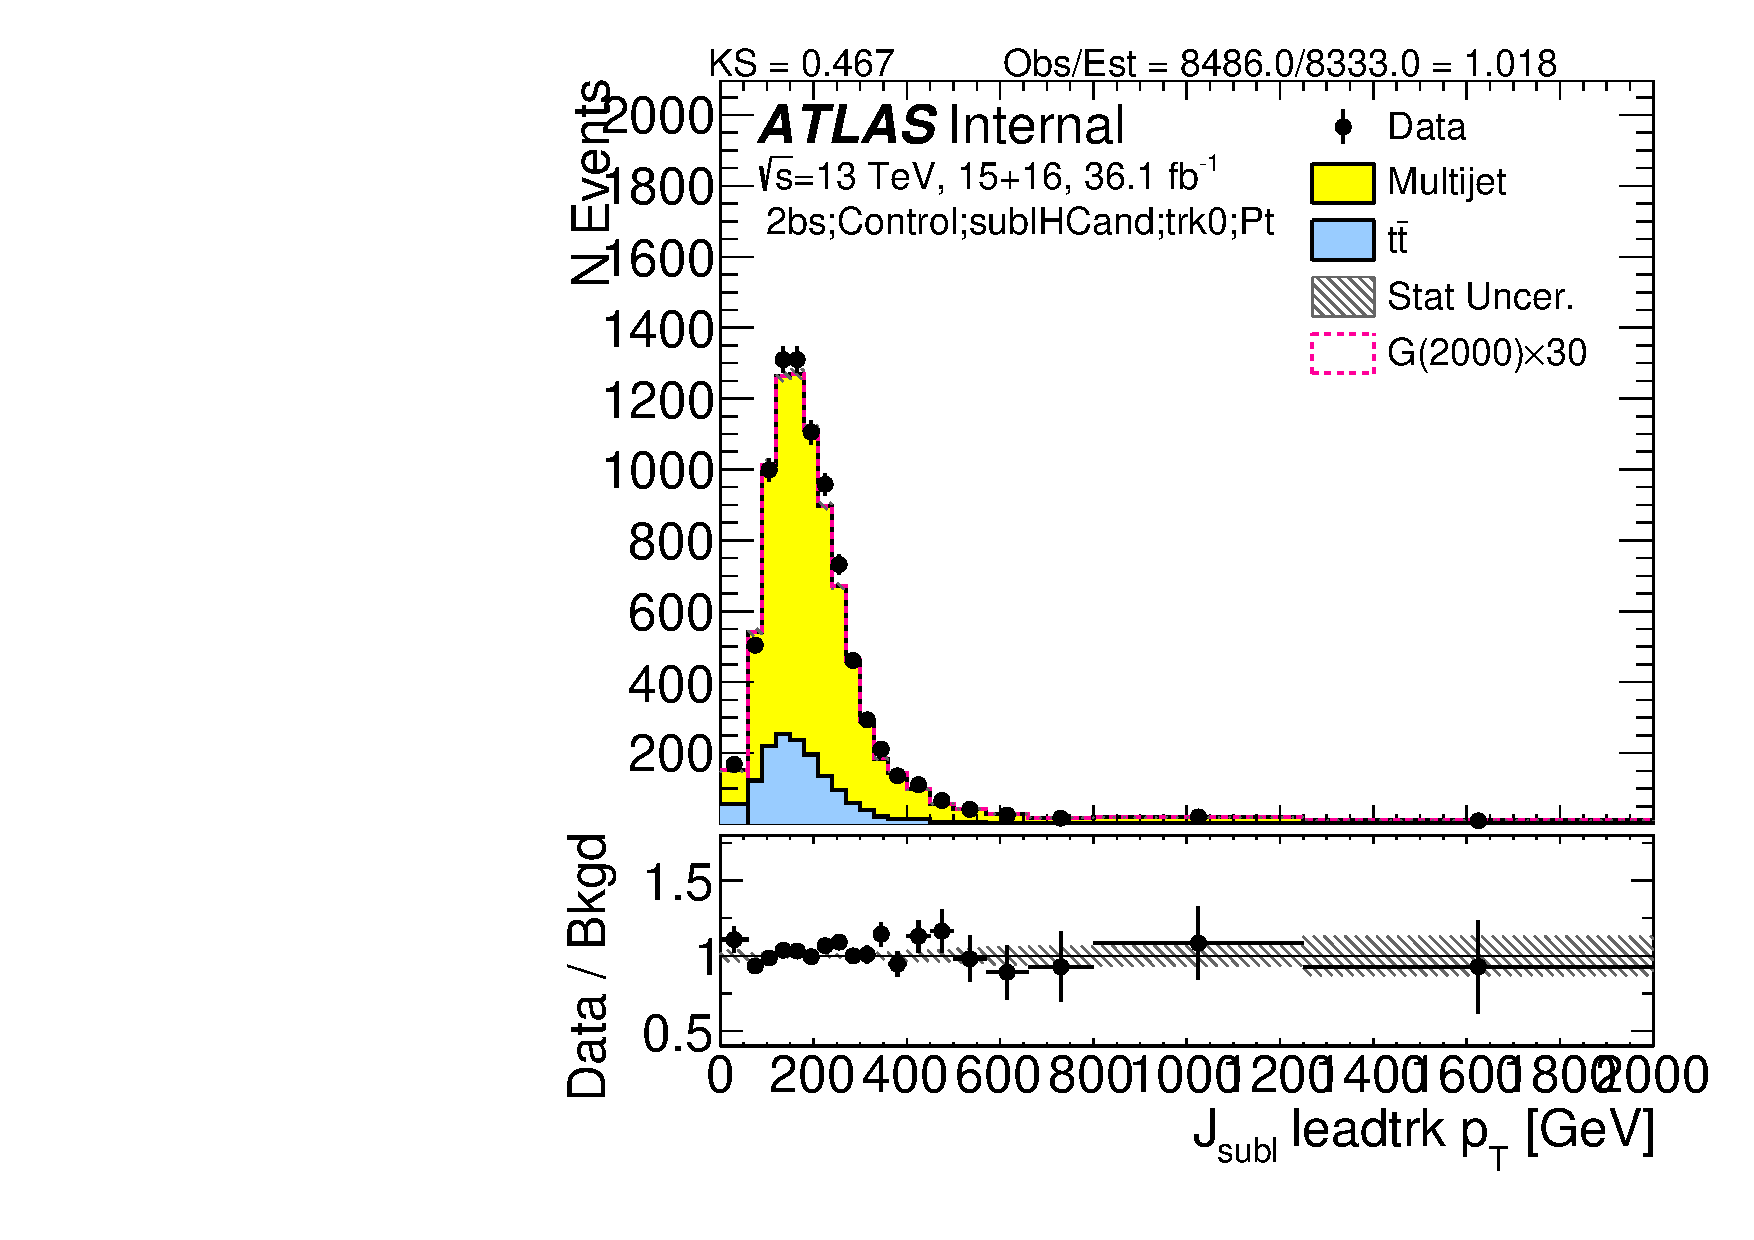
\includegraphics[width=0.32\textwidth,angle=-90]{figures/boosted/Control/b77_TwoTag_split_Control_sublHCand_trk0_Pt.pdf}
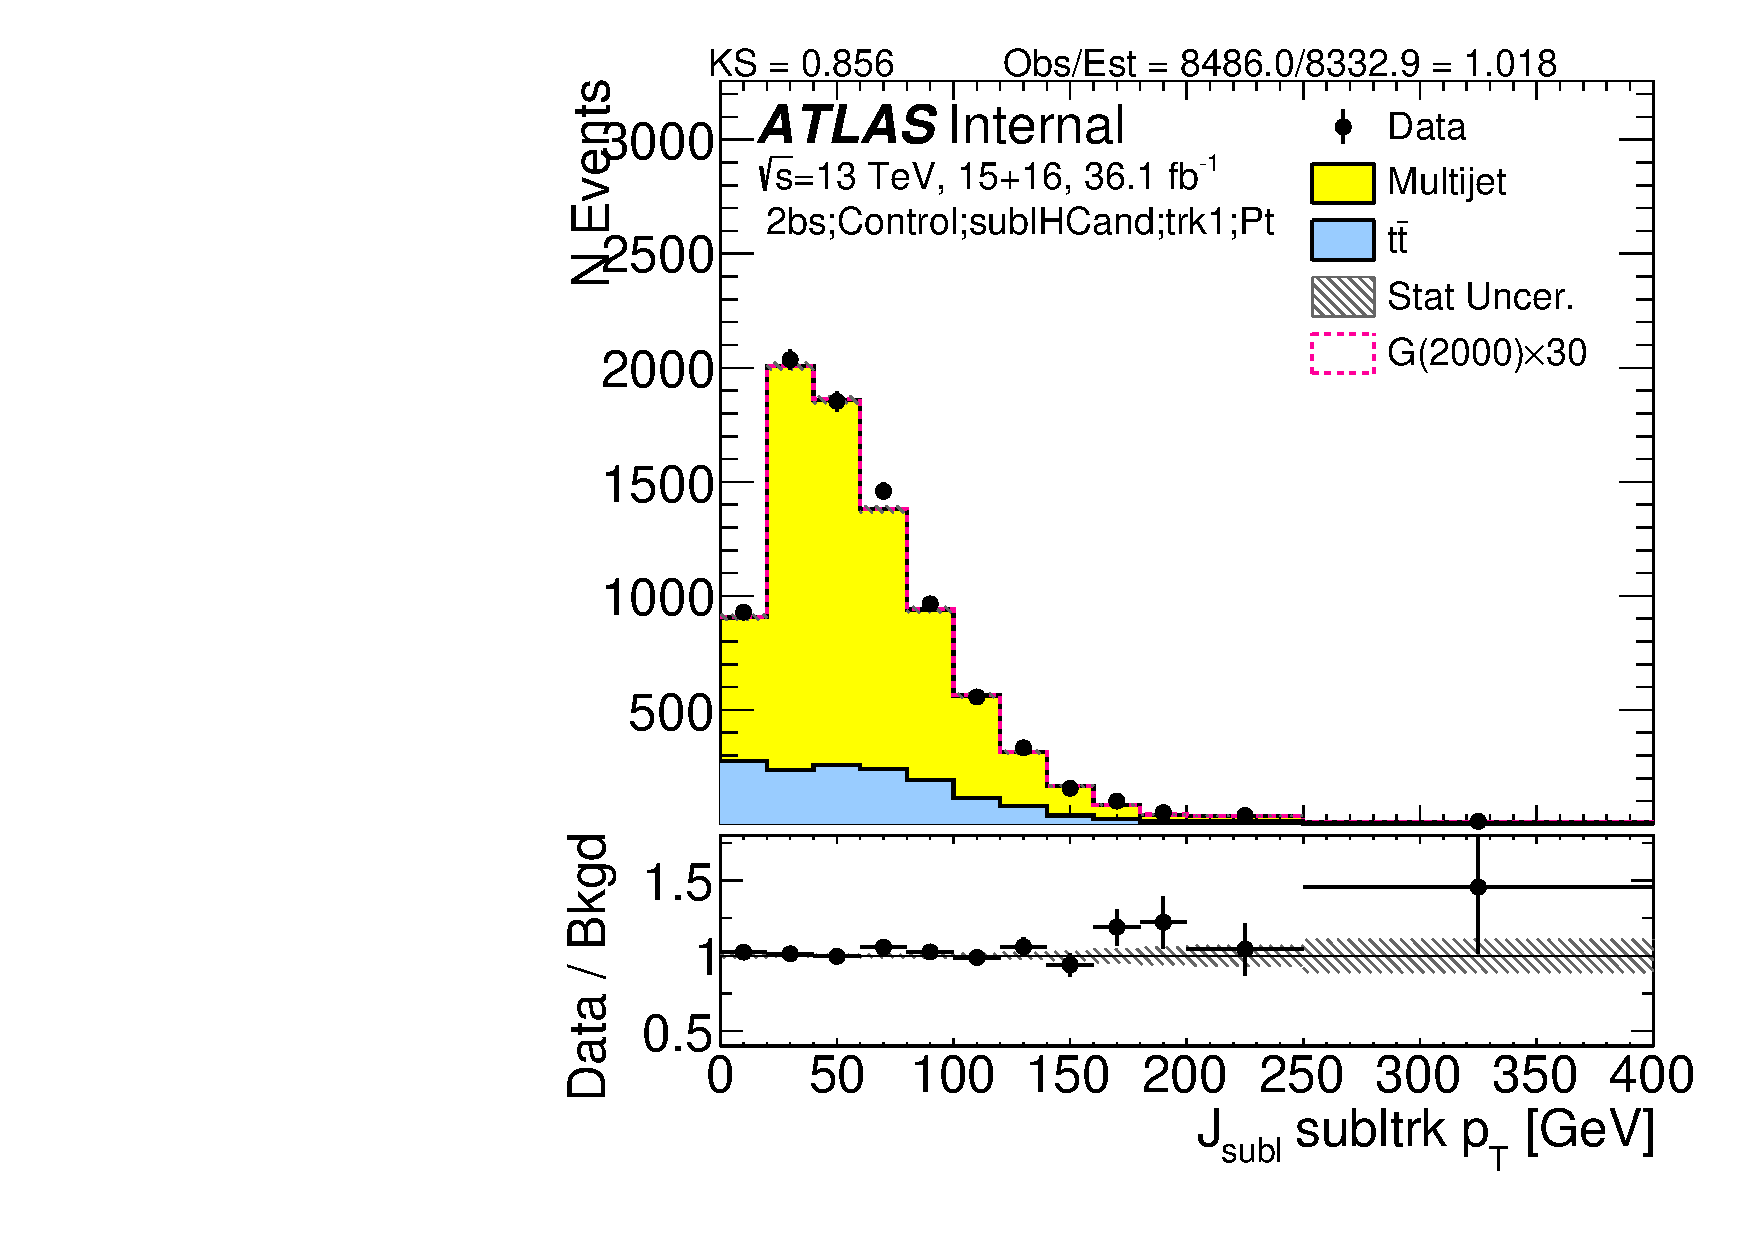
\includegraphics[width=0.32\textwidth,angle=-90]{figures/boosted/Control/b77_TwoTag_split_Control_sublHCand_trk1_Pt.pdf}\\
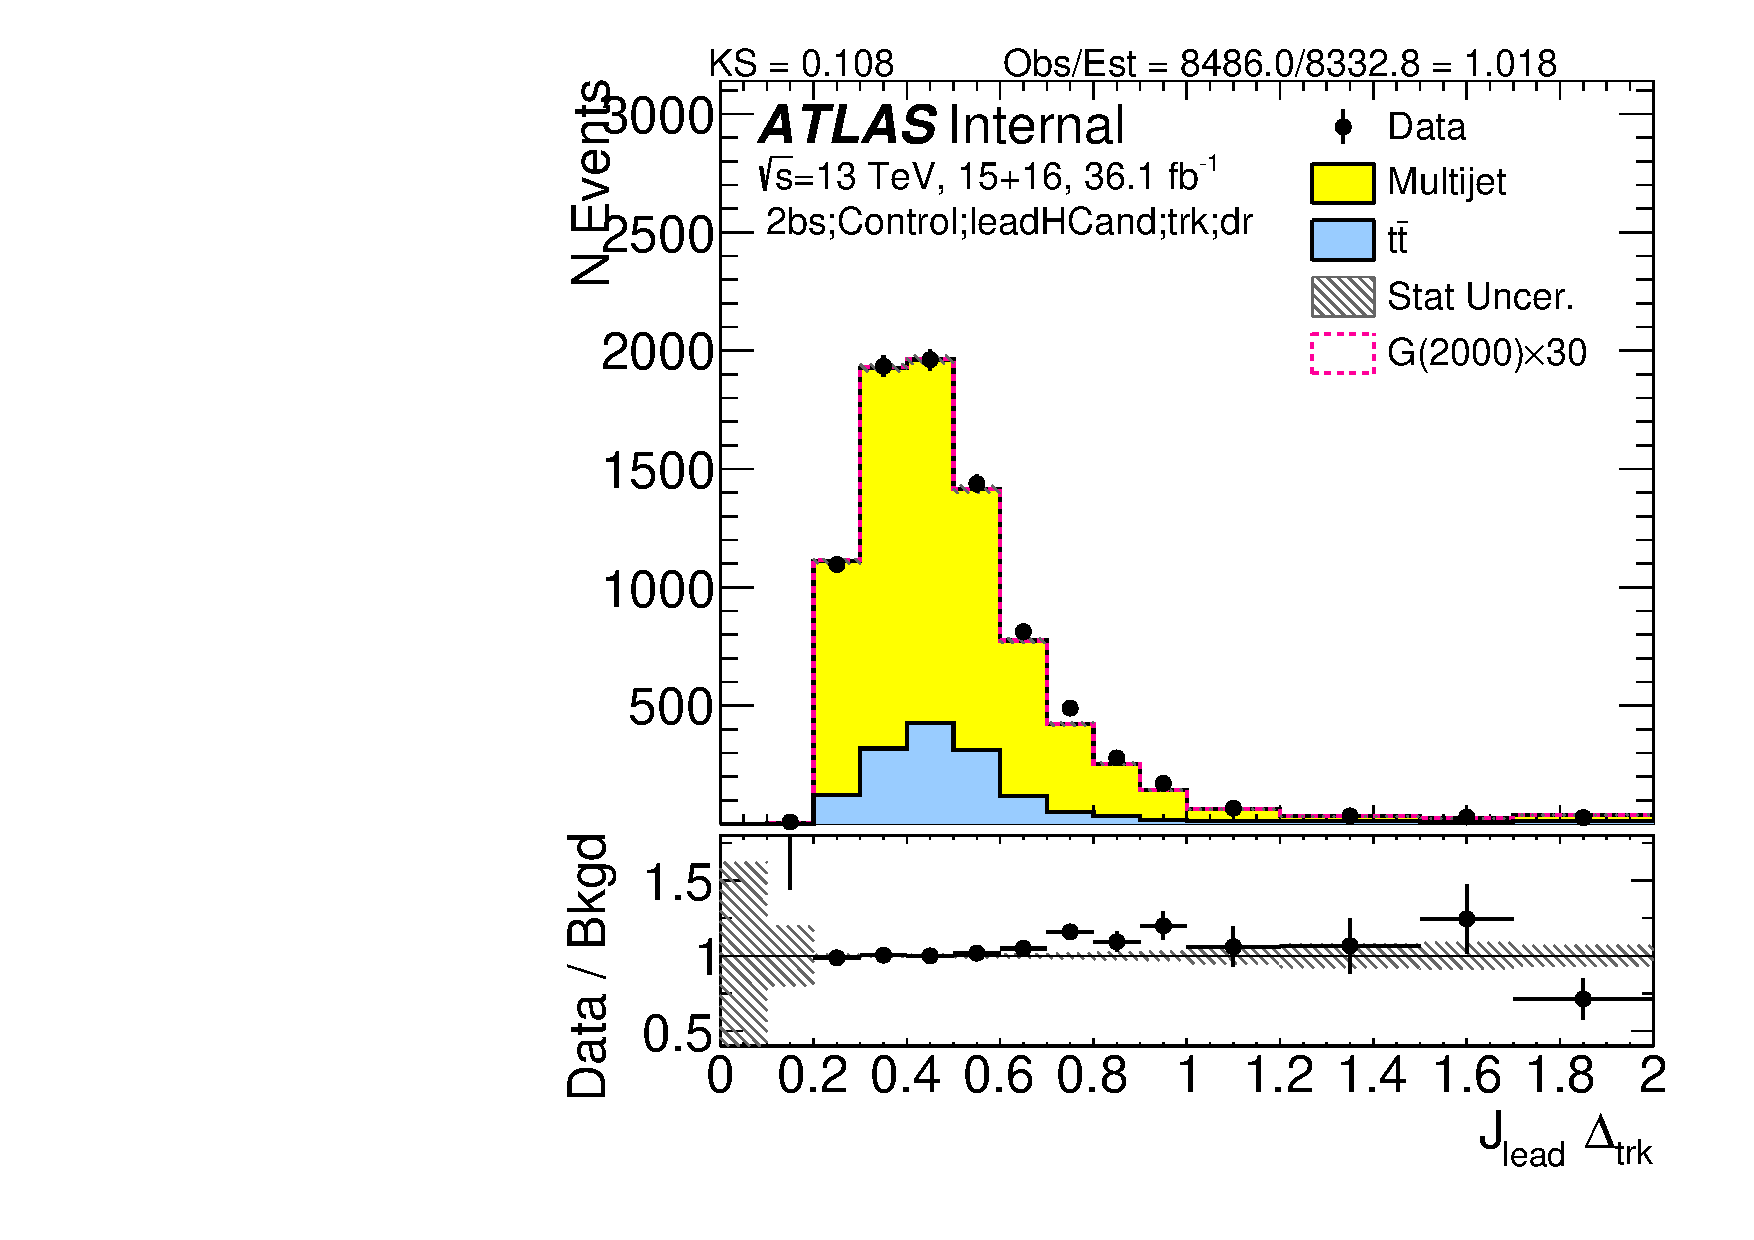
\includegraphics[width=0.32\textwidth,angle=-90]{figures/boosted/Control/b77_TwoTag_split_Control_leadHCand_trk_dr.pdf}
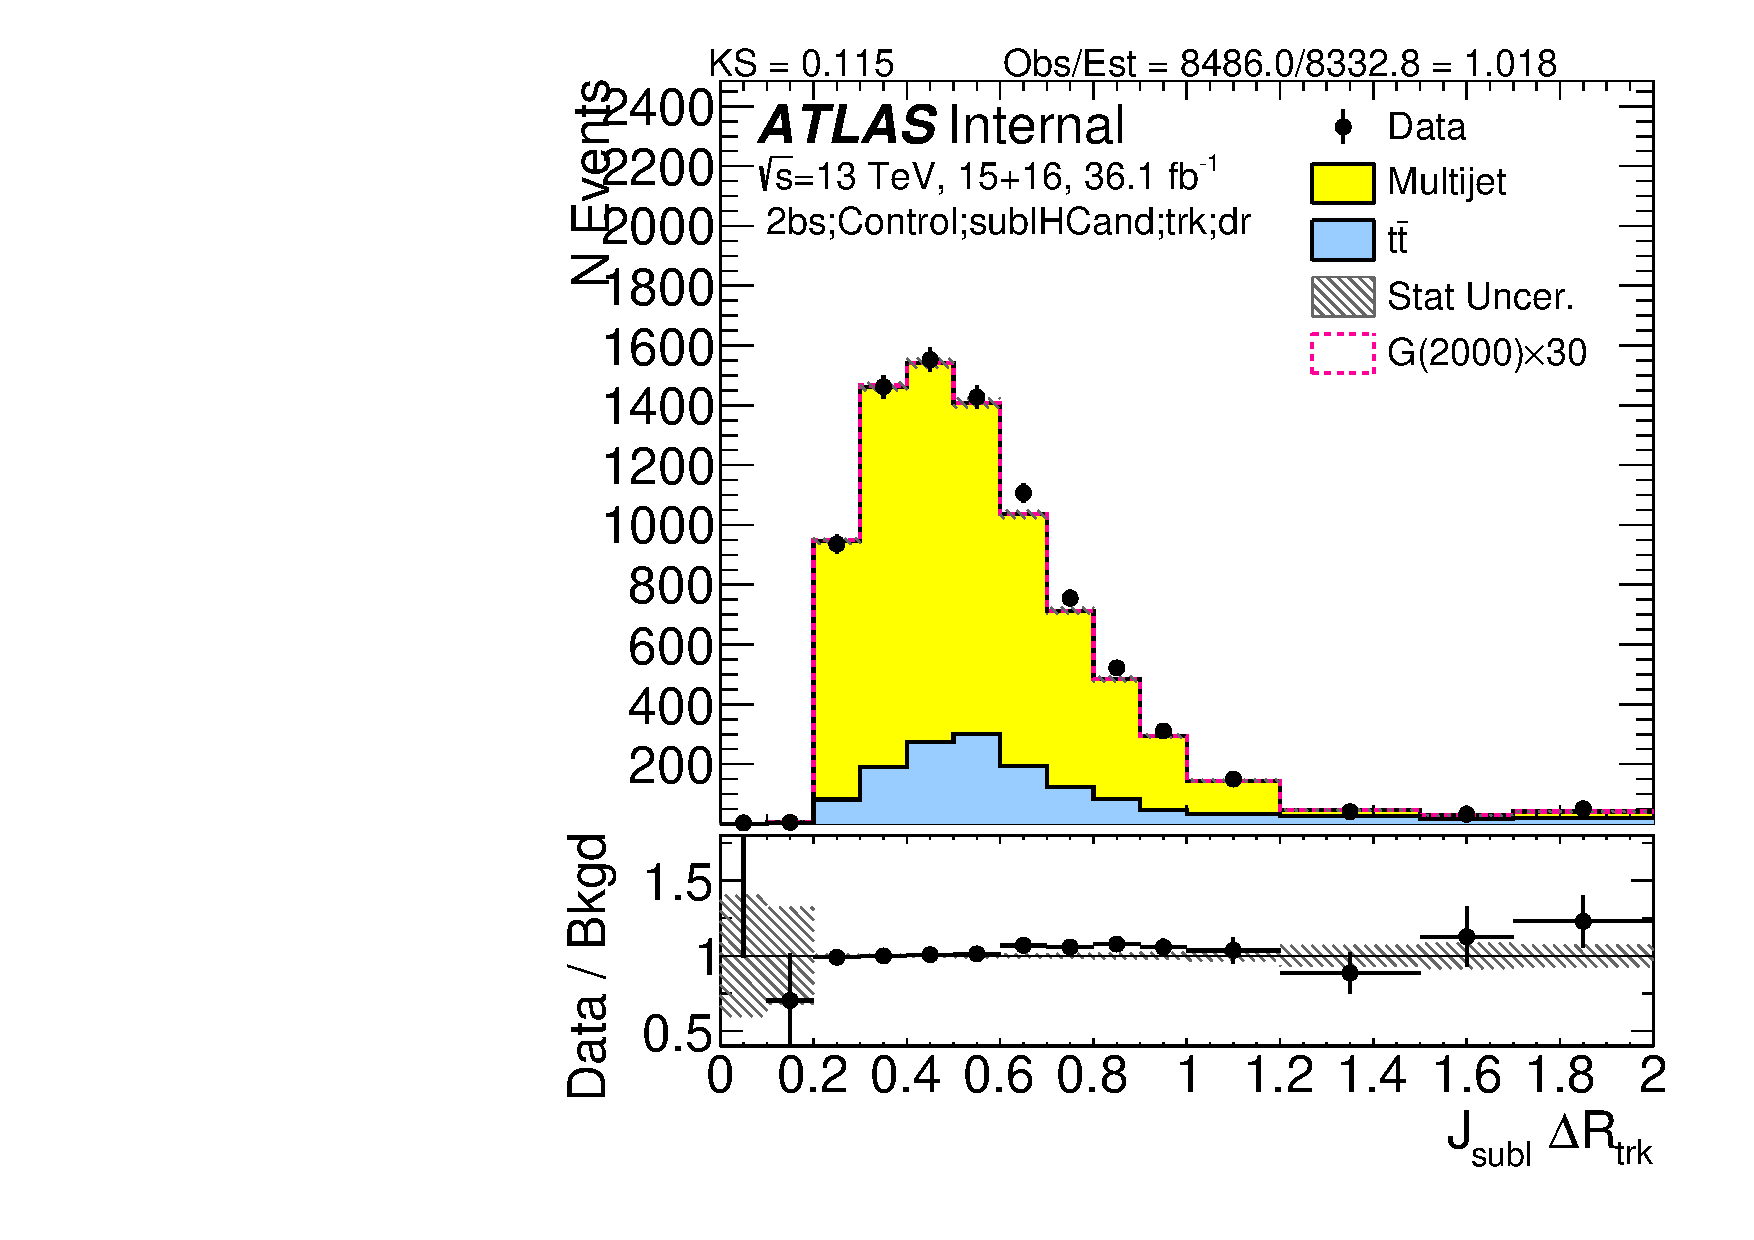
\includegraphics[width=0.32\textwidth,angle=-90]{figures/boosted/Control/b77_TwoTag_split_Control_sublHCand_trk_dr.pdf}
  \caption{First two rows show the kinematics of the lead (left) and sub-lead (right) small-$R$ track jets associated to the lead (first-row) and sub-lead (second-row) large-\R jet in data and prediction in the control region after requiring 2 $b$-tags split. Third row shows the $\Delta R$ between two leading small-$R$ track-jets associated to the leading (left) and sub-leading (right) large-\R jet.  }
  \label{fig:boosted-2bs-control-ak2}
\end{center}
\end{figure*}


\begin{figure*}[htbp!]
\begin{center}
\includegraphics[width=0.32\textwidth,angle=-90]{figures/boosted/Control/b77_TwoTag_split_Control_mHH_l_1.pdf}
\includegraphics[width=0.32\textwidth,angle=-90]{figures/boosted/Control/b77_TwoTag_split_Control_hCandDr.pdf}\\
\includegraphics[width=0.32\textwidth,angle=-90]{figures/boosted/Control/b77_TwoTag_split_Control_hCandDeta.pdf}
\includegraphics[width=0.32\textwidth,angle=-90]{figures/boosted/Control/b77_TwoTag_split_Control_hCandDphi.pdf}
  \caption{Kinematics of the large-\R jet system in data and prediction in the control region after requiring 2 $b$-tags split.  }
  \label{fig:boosted-2bs-control-ak10-system}
\end{center}
\end{figure*}